\documentclass{article}

\usepackage[table]{xcolor}
\usepackage[HTML]{xcolor}
\usepackage[utf8]{inputenc}
\usepackage[T1]{fontenc}
\usepackage[table]{xcolor} 
\usepackage{tabularx}
\usepackage{multirow}
\usepackage{amsmath}
\usepackage{adjustbox}
\usepackage{amssymb}
\usepackage{graphicx}
\usepackage{svg}
\usepackage[margin=1in]{geometry}
\usepackage{booktabs}
\usepackage{array}
\usepackage{pdflscape}
\newcolumntype{L}{>{\columncolor{gray!15}\raggedright\arraybackslash\bfseries}p{4cm}}
\newcolumntype{C}{>{\centering\arraybackslash}X}
\newcolumntype{R}{>{\raggedleft\arraybackslash}X}
\usepackage{blindtext}
\usepackage{tikz}
\usetikzlibrary{trees}
\usepackage{minted} 
\usepackage{fancyhdr}
\usepackage[colorlinks=true, linkcolor=gray, urlcolor=gray, citecolor=gray, filecolor=gray]{hyperref}
\newcommand{\obsub}[1]{%
  \stepcounter{OBnum}%
  \addcontentsline{toc}{subsubsection}{OB \arabic{OBnum} - #1}%
  \subsection*{OB \arabic{OBnum} - #1}%
}
\newcounter{OBnum}

% --- 6. HEADER & FOOTER ---
\pagestyle{fancy}
\fancyhf{} 
\setlength{\headheight}{20pt} % Increased for two lines
\fancyhead[R]{104 - Team Not Found \\ version 1.0}\fancyfoot[C]{\thepage}
\fancyfoot[C]{\thepage}
\renewcommand{\headrulewidth}{0.4pt}

\begin{document}
\clearpage
\thispagestyle{empty}
\hbox{}
\clearpage
% --- TITLE PAGE ---
\begin{titlepage}
    \centering 
    {\Huge\bfseries Planning of the software \par}
    \vspace{0.5cm}
    {\Large\itshape the definition of use cases and actual functionalities\par}
    \vspace{2cm}
    
    \begin{figure}[h]
        \centering
        
\includegraphics[width=1.0\textwidth]{104okok.png}
    \end{figure}
    
    \vfill

    % Nome del team centrato e molto grande
    {\Huge \textbf{104 - Team Not Found}} \\
    \vspace{0.55cm}

    \begin{flushright}
        
    
        {\large \textbf{Matteo Golinelli, Caterina Alessi, Robin Bertolini, Virginia Ancora}} \\
        \vspace{0.1cm}
        {\large \textit{ \today}}
    \end{flushright}
\end{titlepage}

\cleardoublepage
\tableofcontents
\newpage
\section{Context Description}
\paragraph{
This document shows the context of the Deliverable 2 of the Tain Web Application project, developed for the Software Engineering course.
}
\paragraph{
Deliverable 2 focuses on the planning part, acting like a sort of intermediary between high-level requirements of the Deliverable 1 and the Deliverable 3: by bringing a detailed, and easy-to-codify design (driven for Deliverable 3).
While Deliverable 1 focuses on what the system should do (with FR and NFR), Deliverable 2 shows how the system will behave, from an external perspective, and how its internal structure will support that behaviour.
It also serves as a corrected and updated version of the content already presented in the Deliverable 1, showing the differences and updates introduced; by resending the new version.
}
\paragraph{The document is written for internal and external users, including our software development team, the Railway-Administration staff, and any external assessors evaluating the completeness and quality of the requirements specification.
}
\newpage
\section{Project Objectives}

The Project Idea originates from the need of many student and train-travelers to improve, modernize, extend already existing Train Application (like "TrenItalia") to better manage the ticket purchase and management of both route ticket and regional subscription (like the TrentinoTrasporti's one) \\
The solution that we have chosen consists in the development of a web-based software  that consolidates ticketing, journey planning, real-time information, and analytics into a single and complete web-app.\\
The Web Application is designed to serve two primary actor groups:
\begin{itemize}
    \item Customers 
    \subitem - Passengers (only registered)
    \subitem - User of the Web-App (both registered and anonymous)
    \item Train Inspectors
\end{itemize}
Specifically, the Web Application will present all the objectives mentioned below.

\obsub{User-Friendly Interface}
\label{OBJ1}
Provide a user-friendly interface for buying, and managing train tickets, and regional or single-route subscriptions passes, modifying existing bookings, and view any their active subscription at any time.\\
It does not cover the issue of physical tickets, physical ticket printing management.

\obsub{Delay prediction}
\label{OBJ2}
Support journey  planning and optimization through intelligent search filters and delay prediction. The Web-App shall allow passengers to search for links, select preferred travel options, and receive prediction of delays before booking the travel, in order to simplify the organization of other journey or exchanges with other means of transportation.\\
It does not cover the guaranty of real arrival times prediction.

\obsub{Additional Travel-Related booking}
\label{OBJ3}
Allow passengers to book additional travel-related services, including on-board luggage storage, and dedicated bike wagon spaces for bikes and e-bikes.\\
It does not cover the actual operational aspects; it handles only the reservation, not the actual assignment of the actual assigned numbered place reserved.

\obsub{Real-Time Train Information}
\label{OBJ4}
Provide real-time train information, including live occupancy conditions of the wagons and departure/arrival boards, enabling passengers to make informed decisions before their journey.\\
It does not cover historical occupancy analytics or predictive crowding forecasts other than the real-time feed provided by the ticket inspector, which will mark the seats as busy when he validates the ticket/subscription.


\obsub{Track Travel-History}
\label{OBJ5}
Allow registered passengers to track their travel history and participate in some internal loyalty programs, accumulating and viewing loyalty points, linked to their past journeys, with the possibility of converting them into discounts or small gifts.\\
It does not address integration with external loyalty ecosystems other than those that are in our Web-App.

\obsub{Ticket Validation}
\label{OBJ6}
Equip train-inspectors with tools to validate passenger tickets and subscriptions, and to monitor real-time wagon occupancy during service.\\
It does not cover automated gate validation hardware integration or penalty fee management. It does not cover the tap-and-go option of ticket payment.
\obsub{Customer-Support and Refunding }
\label{OBJ7}
Provide the service for the customers to contact the support and ask for information, report something that went wrong and ask for refunding .\\
It does not cover the possibility of changing a  ticket, after the established time defined by internal rules.
\obsub{Shift Schedule for Ticket Inspectors}
\label{OBJ8}
Equip Train Inspectors with the shift schedule to know which train they have to work on everyday.\\
It does not cover the implementation of the possibility of expressing preferences on the place where you work daily.

\obsub{Statistic and Insights for administrative staff}
\label{OBJ9}
Equip Railway Managers with a set of tools to visualize and analyze data and statistics about the train company.\\
It does not develop any type of prediction or action-driven suggestion for future financial actions to be done by the Railway Managers.

\newpage
\section{Stakeholders}
% =============================================================================

A stakeholder is anyone or anything that cares about the project or is affected by it. They are essential for shaping the software requirements because their needs tell us what features to build and who we are building them for.
It is also worth noting that a stakeholder is not always a direct user of the application. While some will interact directly with it, others might never touch the software itself but are still heavily affected by its outcomes.

\begin{figure}[htbp] % h=here, t=top, b=bottom, p=page
\begin{center}
\begin{center}
% \resizebox scales the diagram to perfectly fit the width of your page's text area
\resizebox{\textwidth}{!}{%
\begin{tikzpicture}[
  edge from parent fork down,
  grow=down,
  % Global box styling
  every node/.style={draw=black!70, thick, rounded corners, fill=gray!10, font=\sffamily\scriptsize, align=center},
  % Level vertical spacing
  level 1/.style={level distance=1.5cm},
  level 2/.style={level distance=1.5cm},
  level 3/.style={sibling distance=0.95cm, level distance=1.6cm},
  % Specific styles
  root/.style={fill=gray!20, font=\sffamily\bfseries\small, text width=3cm},
  internal/.style={fill=blue!15, font=\sffamily\bfseries, text width=1.8cm},
  external/.style={fill=orange!15, font=\sffamily\bfseries, text width=1.8cm},
  leaf/.style={fill=white, text width=1.3cm, inner sep=2pt},
  lowleaf/.style={fill=white, text width=1.3cm, inner sep=2pt, yshift=-1.3cm}
]

\node[root] {Stakeholders}
  % Wide gap to separate the massive Internal and External trees
  child[sibling distance=11.5cm] {node[internal] {Internal}
    % Custom gap for Internal's children
    child[sibling distance=5.8cm] {node[internal, fill=blue!5] {Human}
      child {node[lowleaf] {Train\\Staff}}
      child {node[leaf] {Customer\\Service}}
      child {node[lowleaf] {IT Ops\\\& Dev}}
    }
    child[sibling distance=5.8cm] {node[internal, fill=blue!5] {Non-Human}
      child {node[leaf] {Train\\Database}}
      child {node[lowleaf] {Train\\Mgmt}}
      child {node[leaf] {Track\\Sensors}}
      child {node[lowleaf] {Ticketing\\Database}}
      child {node[leaf] {Delay\\Predictor}}
    }
  }
  child[sibling distance=11.5cm] {node[external] {External}
    % Custom gap for External's children (smaller because there are fewer boxes)
    child[sibling distance=4.5cm] {node[external, fill=orange!5] {Human}
      child {node[lowleaf] {Railway\\Mgmt}}
      child {node[leaf] {Passengers}}
    }
    child[sibling distance=4.5cm] {node[external, fill=orange!5] {Non-Human}
      child {node[lowleaf] {Payment\\API}}
      child {node[leaf] {Mapping\\API}}
      child {node[lowleaf] {Login\\API}}
    }
  };

\end{tikzpicture}%
}
\end{center}
\end{center}
\caption{Stakeholder graph}
\end{figure}

\subsection{INTERNAL}
Inside the organization or development team. Directly involved in building or governing the system.

\subsubsection*{- Human}
People who interact directly or indirectly with the system.
\begin{itemize} 
    \item \textbf{Train staff (Ticket inspector)} \label{STK2}, on-the-ground staff. They interact with the system to check passenger tickets, needing real-time updates on availability and platform changes.
    \item \textbf{Customer Service} \label{STK3}, the team that handles customer support and operations. They need access to user profiles to fix ticketing issues, manage subscriptions, and help passengers. 
    \item \textbf{IT operations and development team} \label{STK5}, the technical staff responsible for the long-term health of the software. They are the primary stakeholders for the 'scalability and maintainability' requirements, needing clean code architecture and monitoring tools.
\end{itemize}

\subsubsection*{- Non-human}
Systems, devices, or services that interact with the system technically.
\begin{itemize}
    \item \textbf{Train database} \label{STK7}, the internal system that stores the physical specifications of the fleet. It is divided into the various types of trains (e.g. regional or InterCity), keeping track of maximum spots available, classes. 
    \item \textbf{Train management system} \label{STK8}, the core operational software that handles live traffic control. Our platform must synchronize with it to ensure the 'when a train leaves' data displayed to users matches reality. 
    \item \textbf{Infrastructure sensors and track control} \label{STK9}, IoT devices positioned at stations and throughout the rail network, they feed real-time data into the system. This constant stream of information keeps timetables and departure times in perfect sync. 
    \item \textbf{Ticketing database} \label{STK10}, the internal storage for all purchases. It has to handle a lot of people buying tickets at the same time so it never accidentally double-books a seat or cargo space.
    \item \textbf{Delay prediction} \label{STK11}, an internal module that analyzes historical data and live track conditions to dynamically update timetables and advise users of expected delays during the booking procedure.
\end{itemize}

\subsection{EXTERNAL}
Outside the organization. Affected by or interacting with the system without building it.

\subsubsection*{- Human}
\begin{itemize}
    \item \textbf{Railway administration/management} \label{STK1}, who assigned the project. Their goal is to obtain the maximum efficiency of the platform by ensuring smooth operations and high accessibility. We provide them with a specific interface to visualize sales and reservation statistics, allowing them to easily monitor current trends.
    \item \textbf{Passengers (registered and anonymous users)} \label{STK12}, the main end-users for the commercial side of the app. Their care about convenience and reliability. They use the platform to check timetables, find their platform, and buy tickets. They expect the system to be highly responsive, even during peak hours.
\end{itemize}

\subsubsection*{- Non-human}
\begin{itemize}
    \item \textbf{Payment gateway API}\label{STK16}, an outside service (e.g., Stripe or PayPal) responsible for handling the financial transactions. Because of the requirement for robustness to concurrent accesses (especially during high-traffic purchasing times), our platform heavily depends on this system's reliability.
    \item \textbf{Mapping and routing API}\label{STK17}, an external service for visually rendering the network. It provides the geographical data necessary to display the list of stations and connections to the users planning their trips.
    \item \textbf{Login API}\label{STK18}, an outside service that takes care of handling the login process and users credentials.
\end{itemize}
\newpage
\vspace{100mm}
\section{Use Case Specifications}
\subsection*{Use Case Diagram}
This diagram describe the main behavior of the system, defining the hierarchy of the actor. We included the main Use Cases of the system.

\begin{figure}[H]
    \centering
    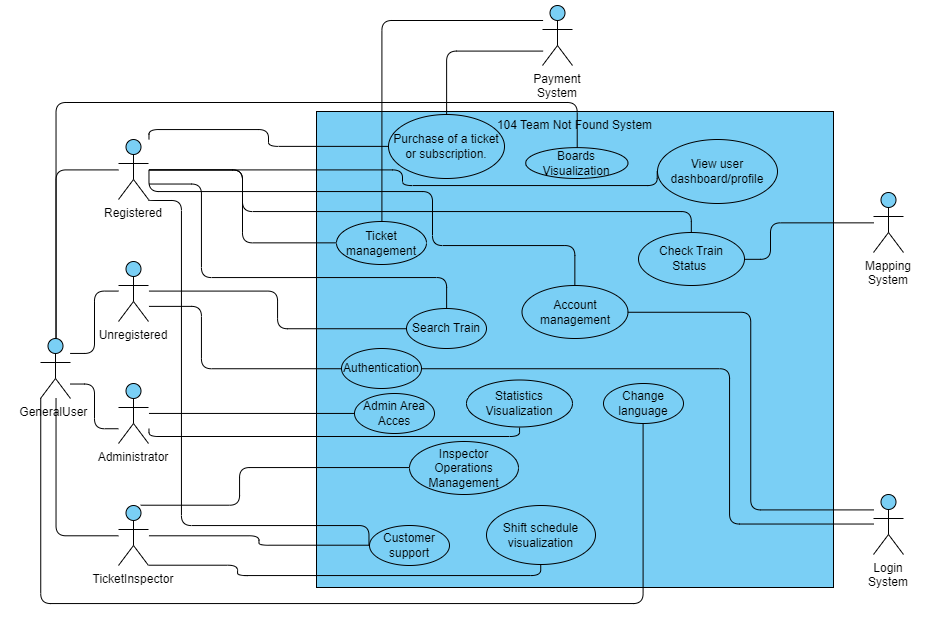
\includegraphics[width=0.9\textwidth]{UseCaseDiagram.png}
\end{figure}
One can observe the actor of the system: 
\begin{itemize}
    \item \textbf{General User} which is any user accessing to the system through any interface, then this actor is divided again in: 
    \begin{itemize}
        \item \textbf{Registered}: Any registered user, which can log-in and buy tickets/subscription
        \item \textbf{Unregistered}: Any visitor of the web-app, can only do basic actions e.g. search trains
        \item \textbf{Administrator}: Person whose in charge of the system, has a dedicated page to see insights on the system
        \item \textbf{Ticket Inspector}: Worker, whose role is to validate ticket and track occupancy on train, has a dedicated page from where he can see his shift schedule and validate tickets or track occupancy
    \end{itemize}
    \item \textbf{Payment System}: System through which our web-app routes payments
    \item \textbf{Login System}: System through which our web-app routes the authentication actions 
    \item \textbf{Mapping System}: System through which our web-app gets data for train position
\end{itemize}
\subsection{UC1: Search Train}
%\textbf{Related Functional Requirements:} FR1, FR2, FR3, FR4, FR5, FR11 
\begin{figure}[H]
    \centering
    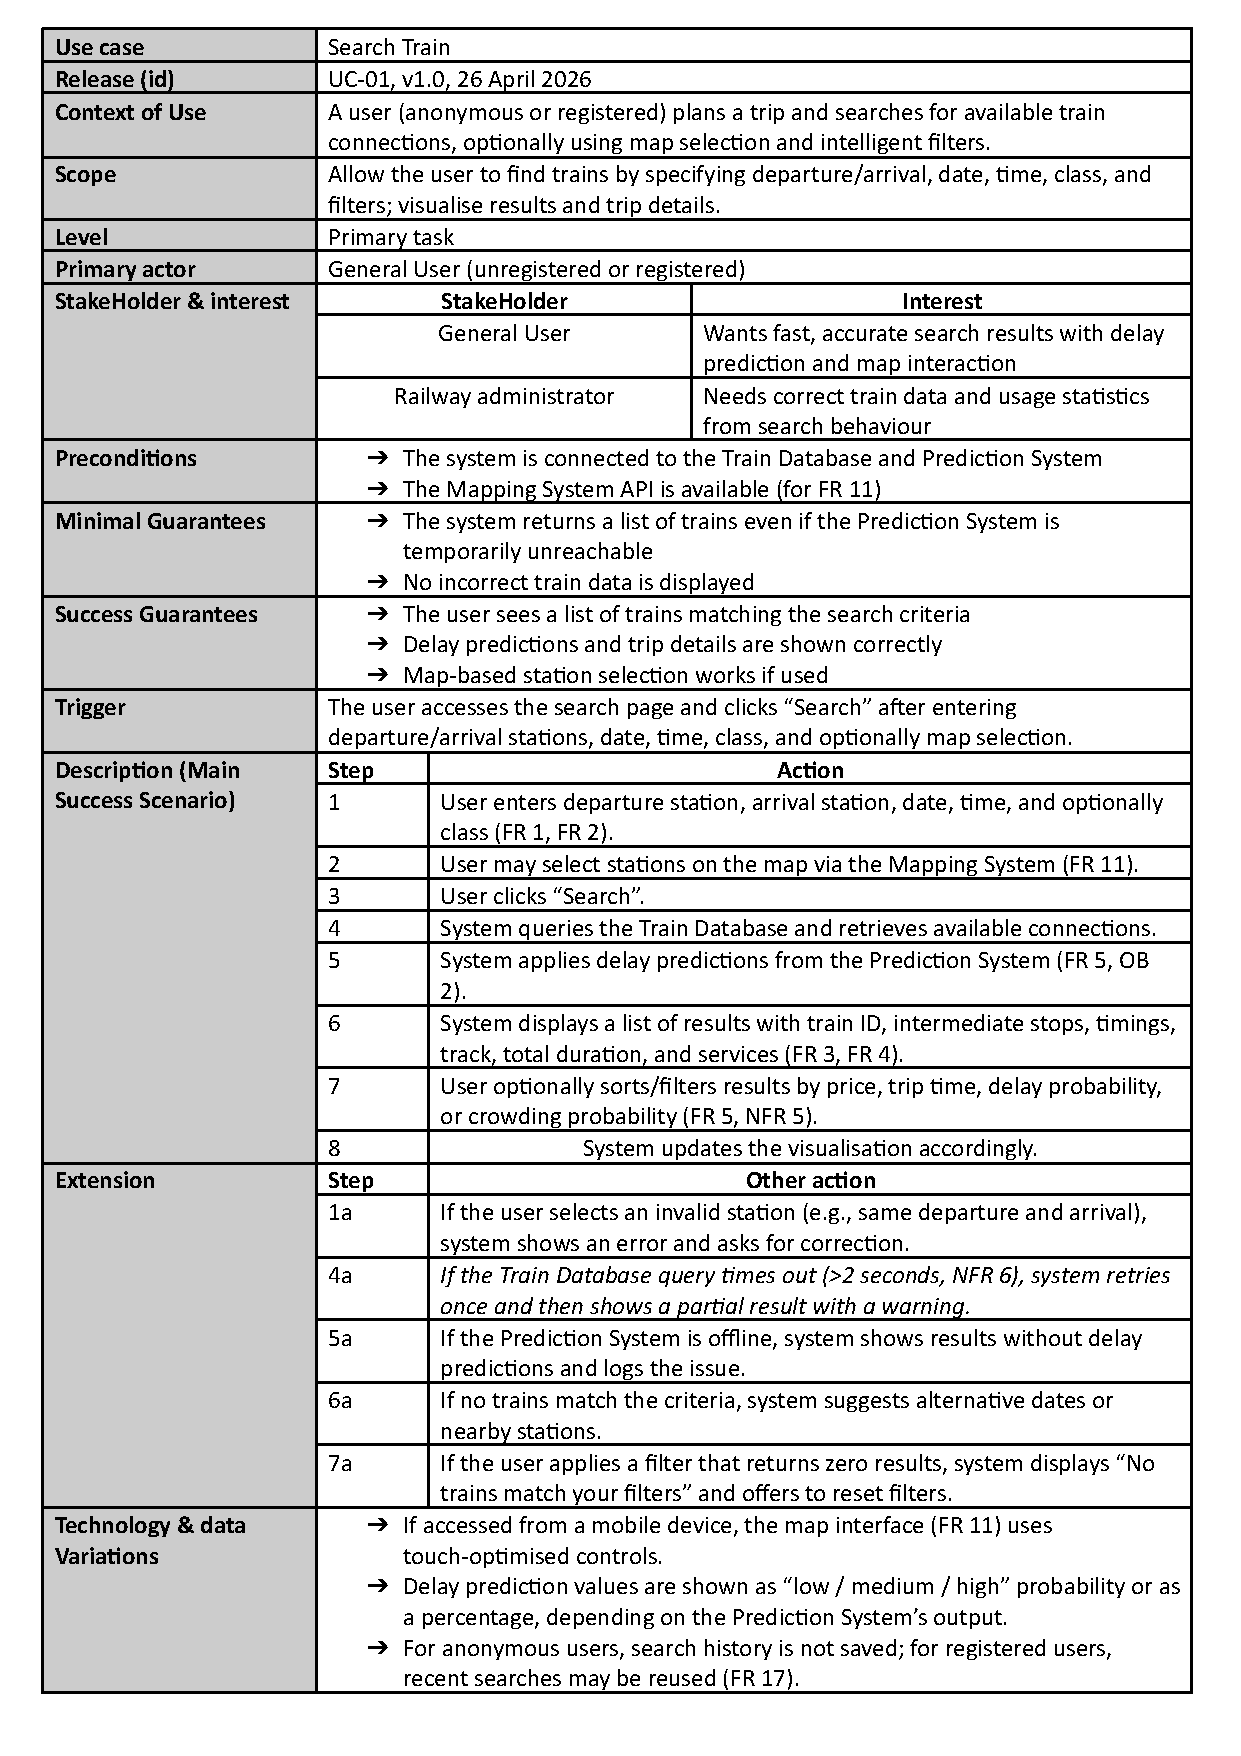
\includegraphics[width=0.9\textwidth]{UC1table.pdf}
\end{figure}
\begin{figure}[H]
    \centering
    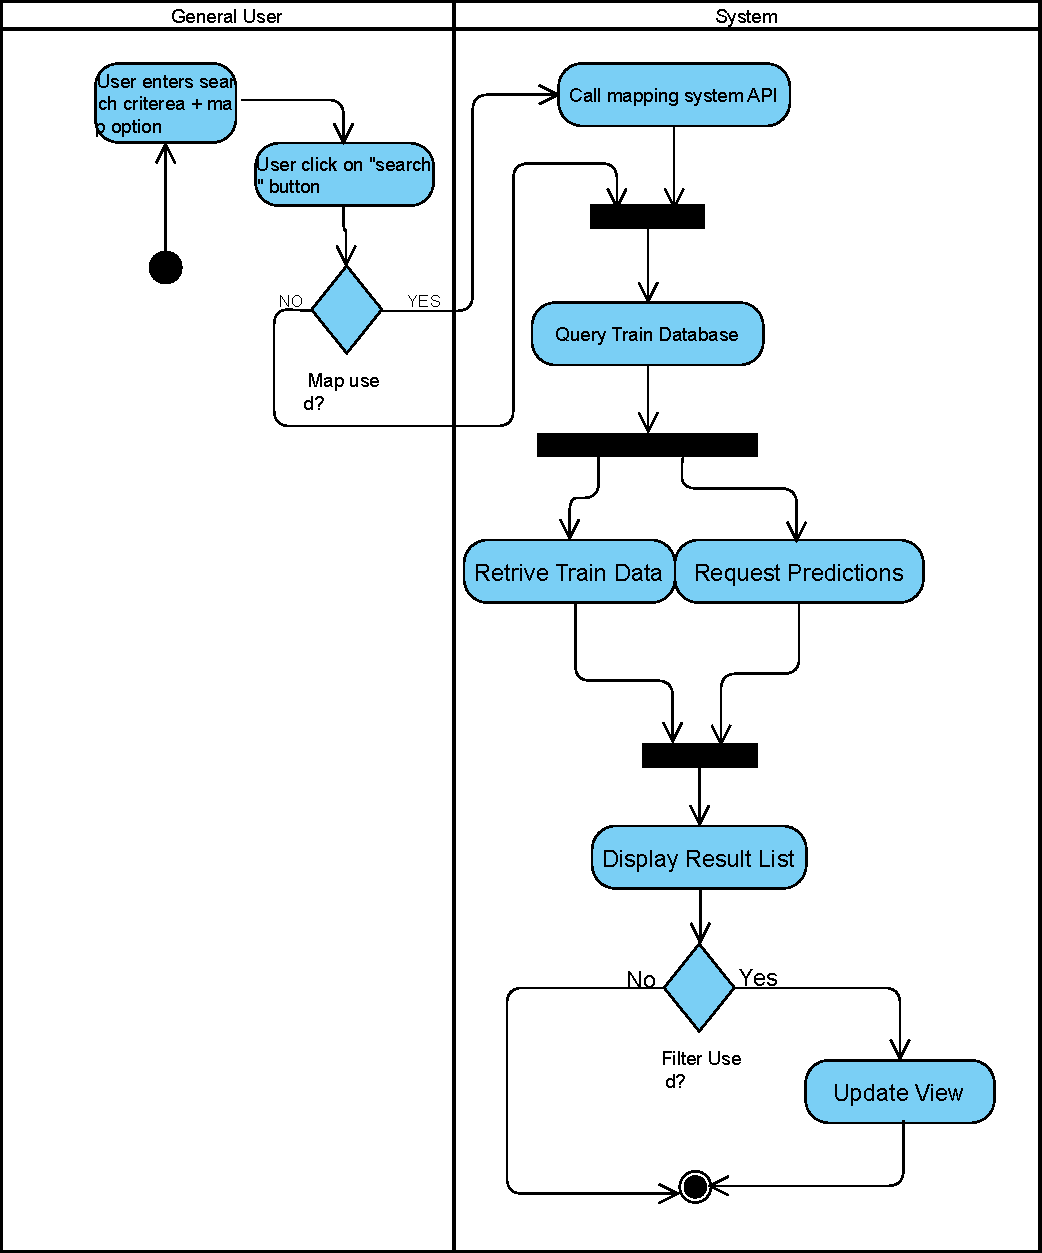
\includegraphics[width=1.0\textwidth]{UC1-activity diagram.pdf}
\end{figure}
\begin{landscape}
\begin{figure}[H]
    \centering
    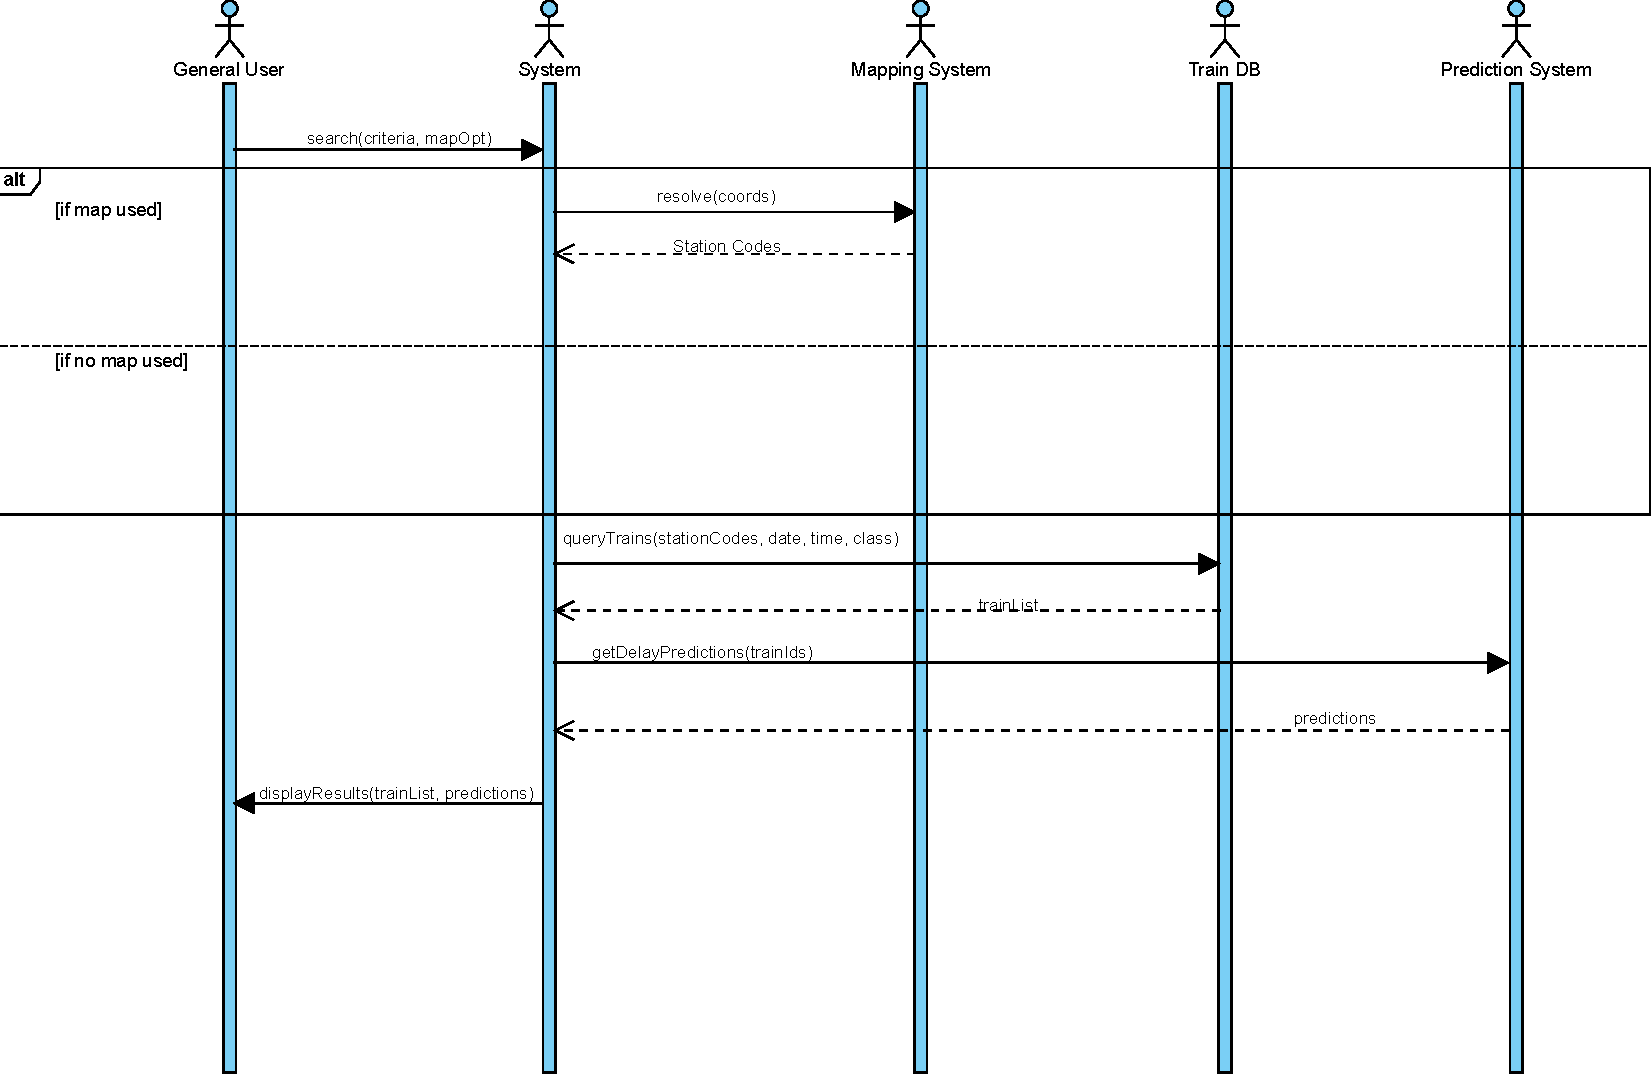
\includegraphics[width=1.3\textwidth]{UC1-sequence diagram.pdf}
\end{figure}
\end{landscape}

\subsection{UC2: Authentication}
%\textbf{Related Functional Requirements:} FR12, FR28, FR34 
\begin{figure}[H]
    \centering
    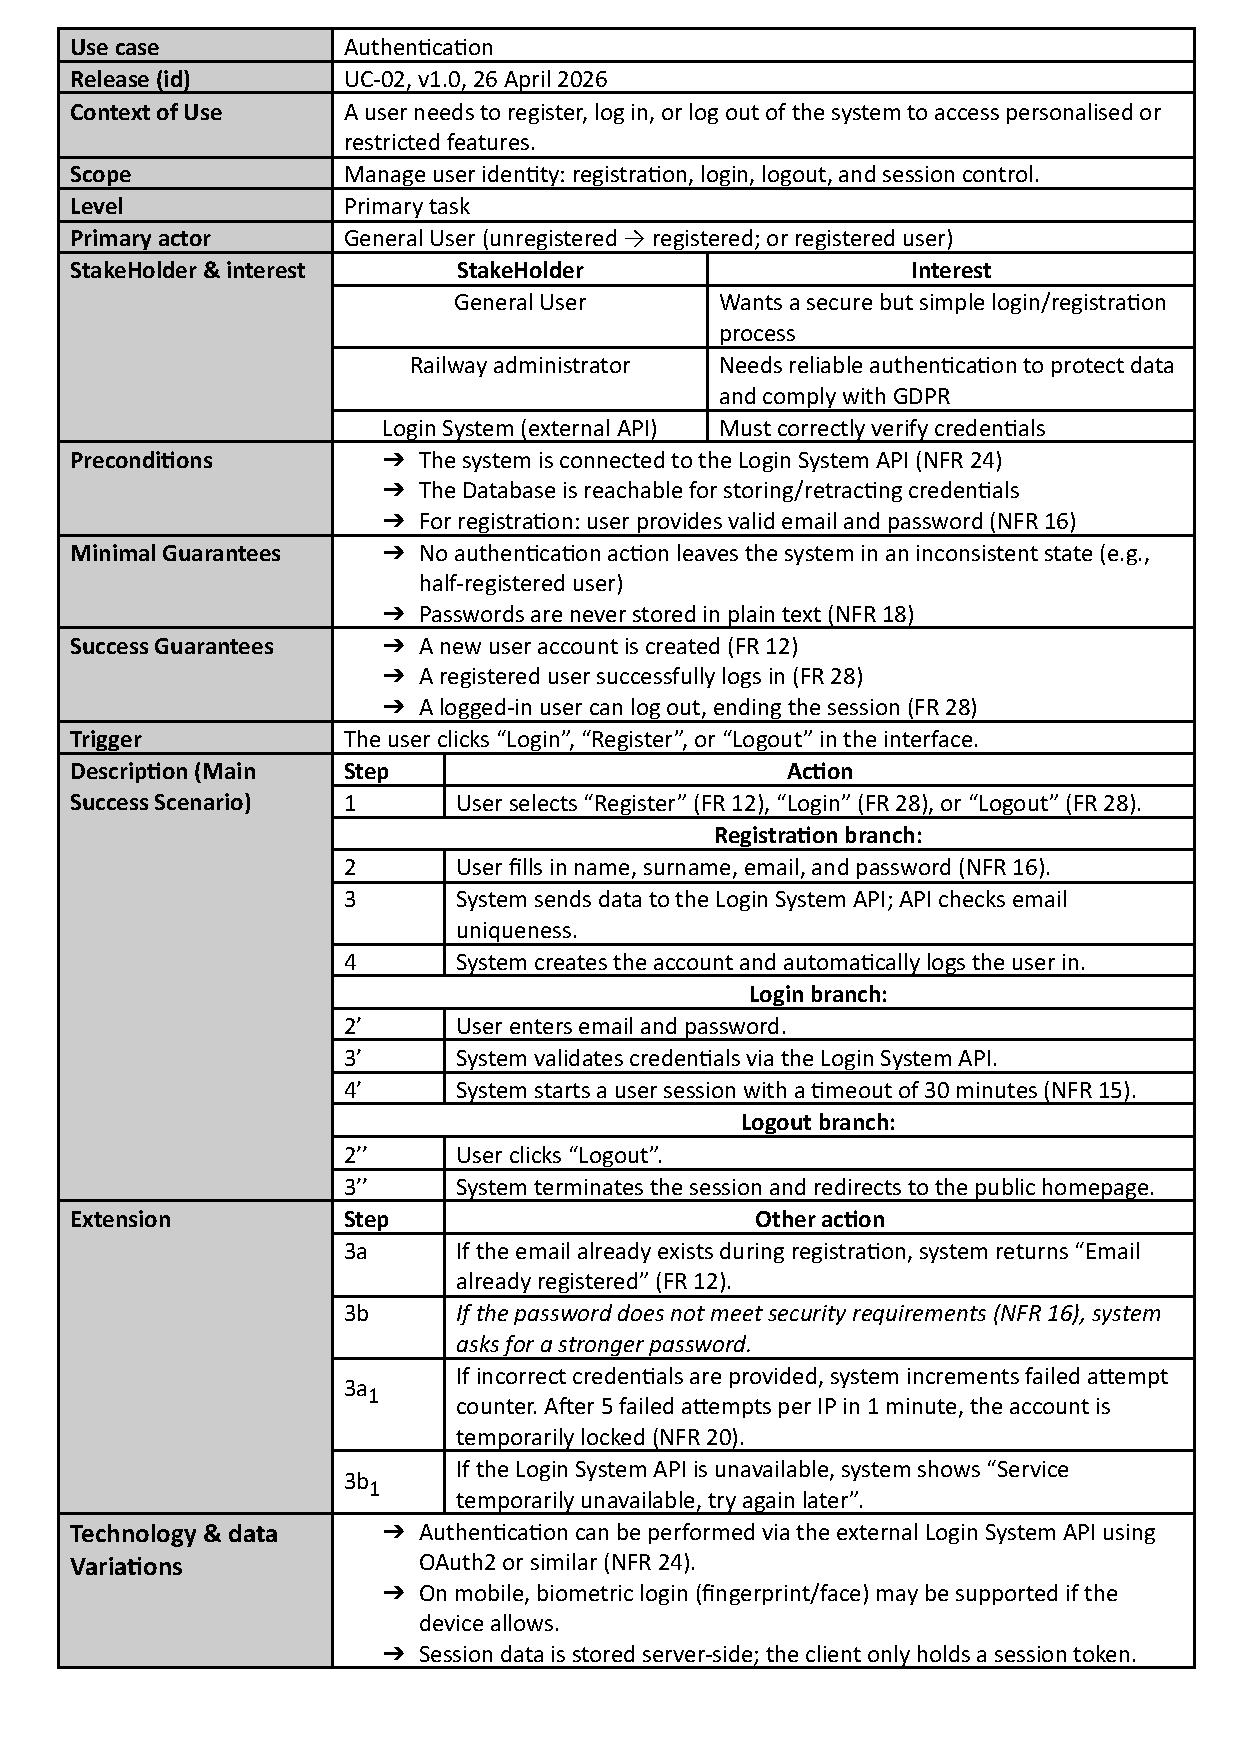
\includegraphics[width=0.9\textwidth]{UC2table.pdf}
\end{figure}
\begin{figure}[H]
    \centering
    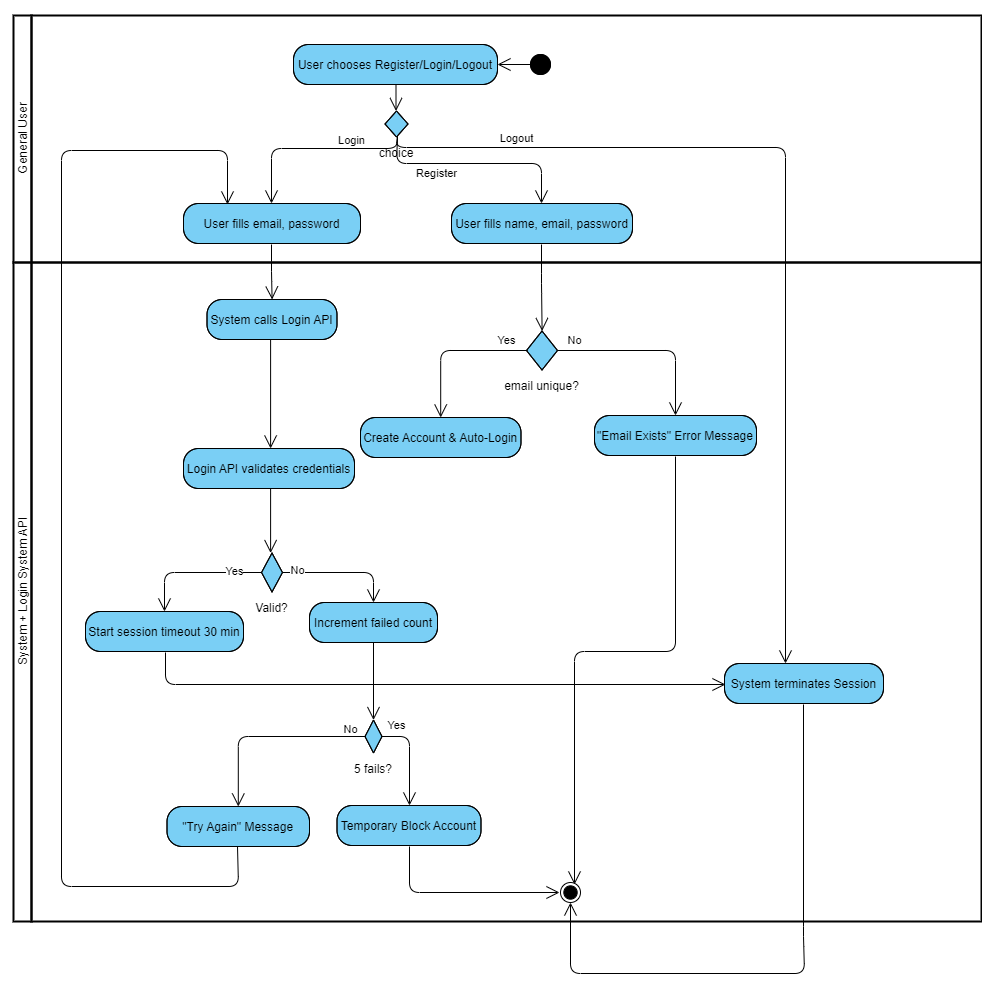
\includegraphics[width=1.0\textwidth]{UC2-activity diagram.png}
\end{figure}

\begin{figure}[H]
    \centering
    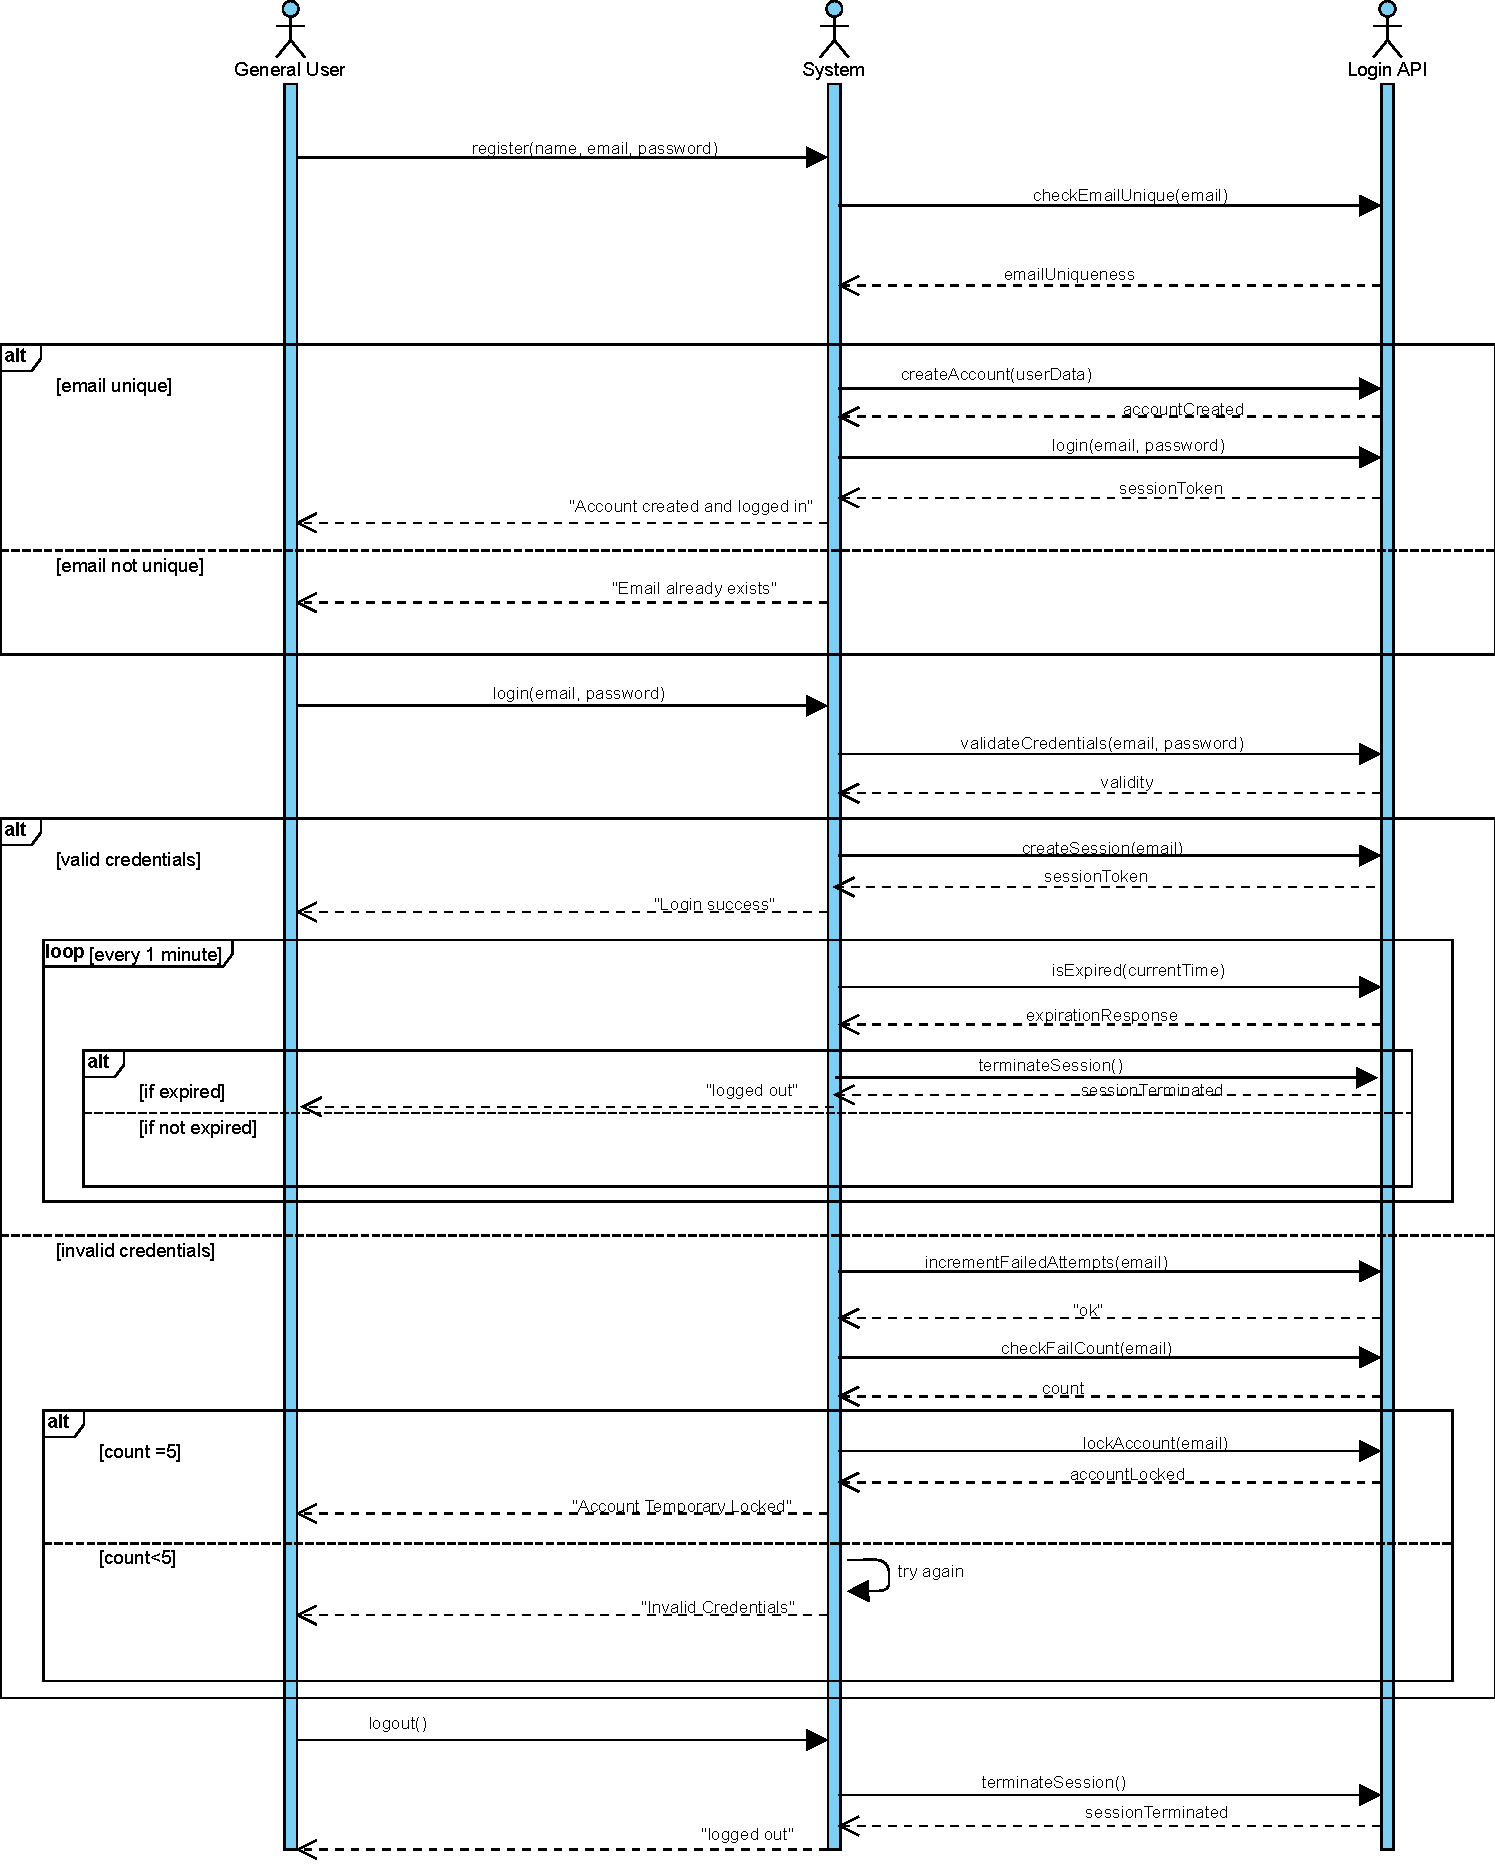
\includegraphics[width=1.0\textwidth]{UC2-sequence diagram.pdf}
\end{figure}

\subsection{UC3: Admin Area Access}
%\textbf{Related Functional Requirements:} FR31 
\begin{figure}[H]
    \centering
    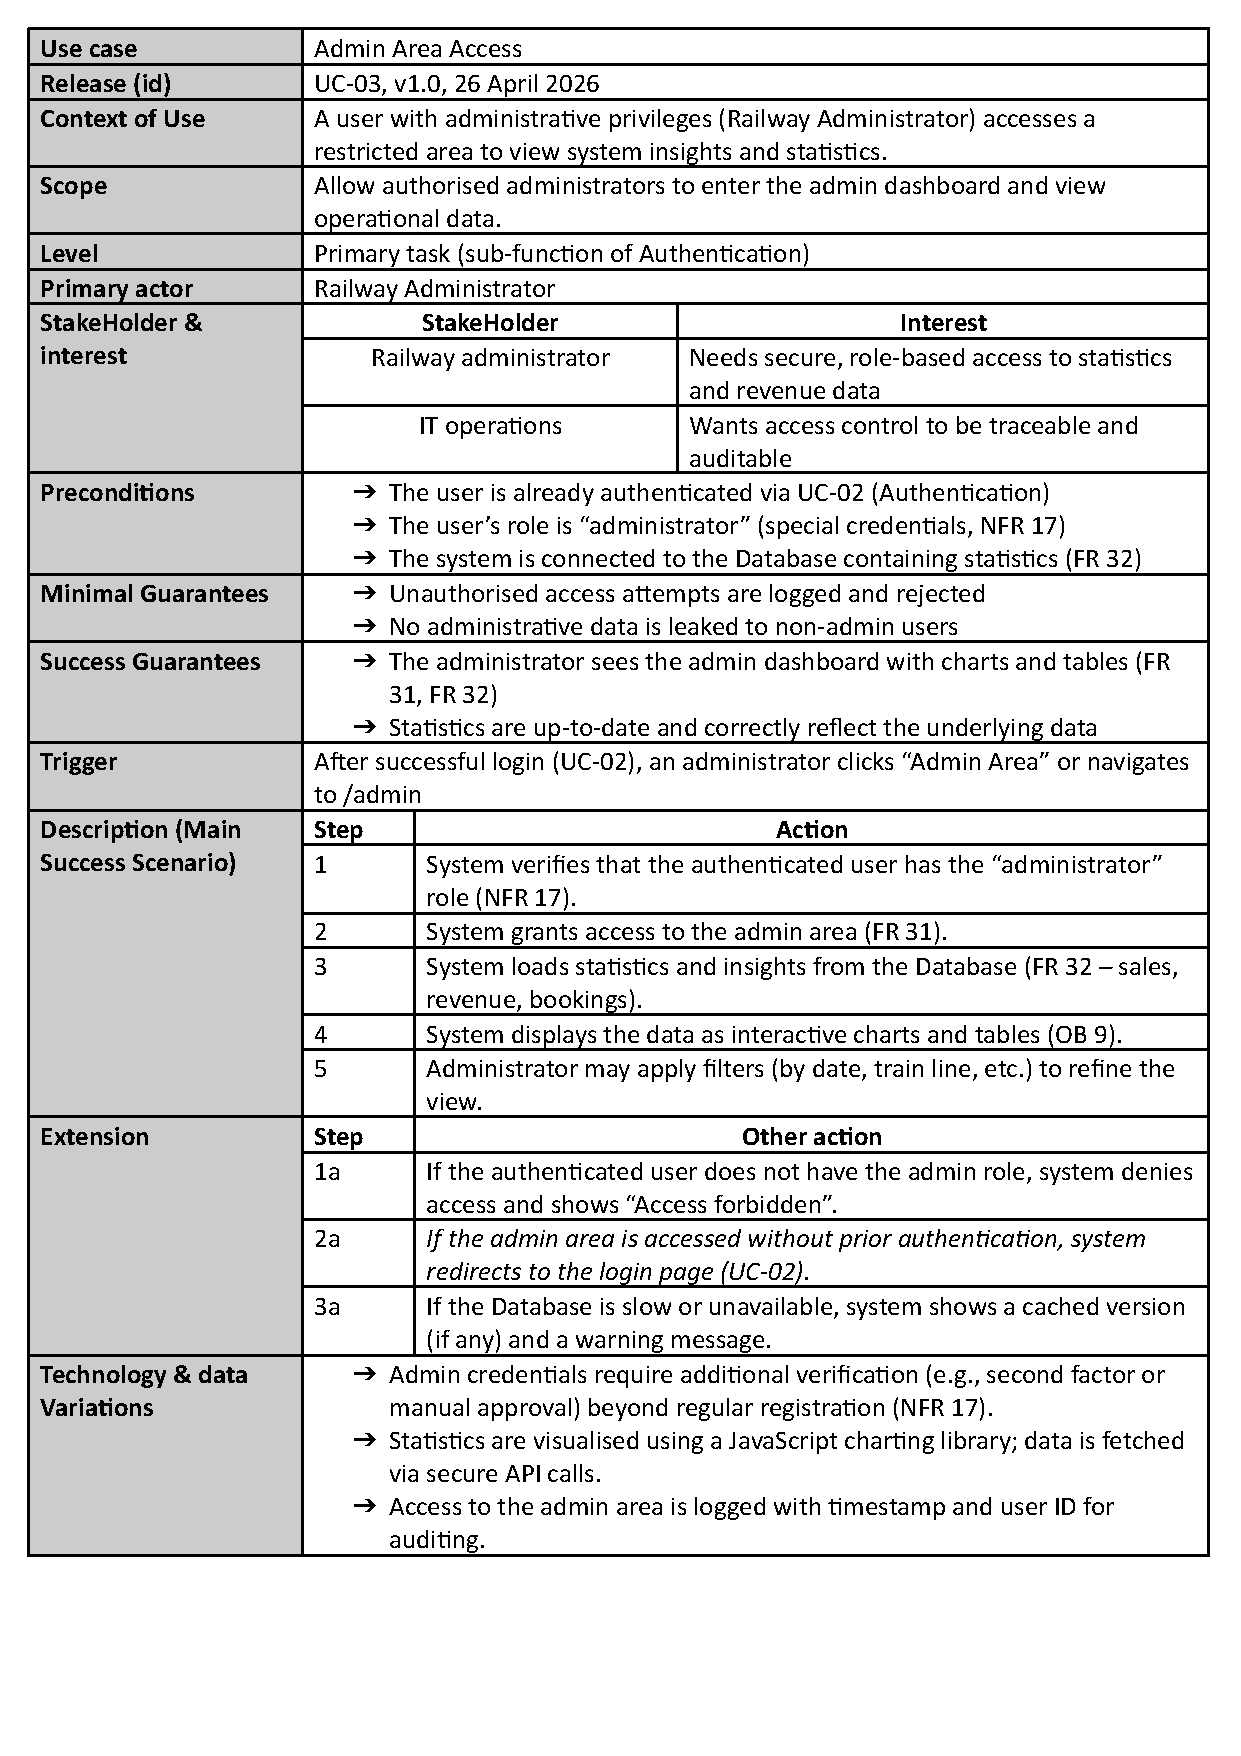
\includegraphics[width=0.9\textwidth]{UC3table.pdf}
\end{figure}
\begin{landscape}
\begin{figure}[H]
    \centering
    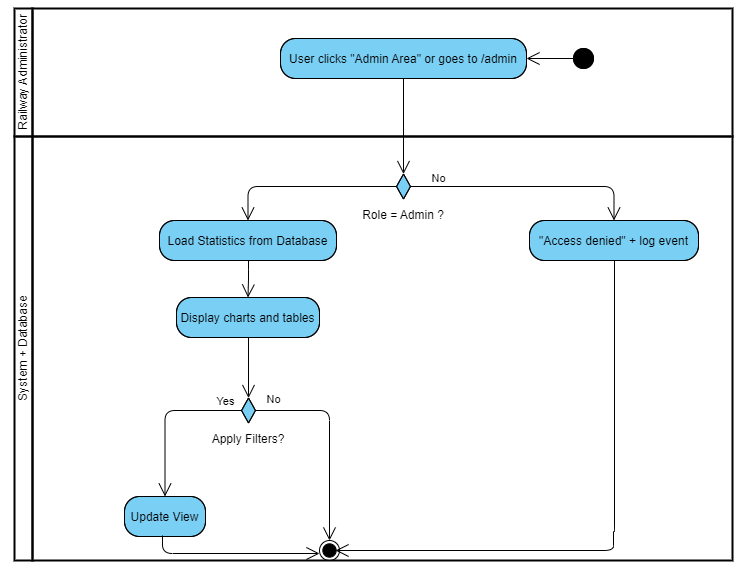
\includegraphics[width=1.2\textwidth]{UC3-activity diagram.png}
\end{figure}
%\end{landscape}
%\begin{landscape}
\begin{figure}[H]
    \centering
    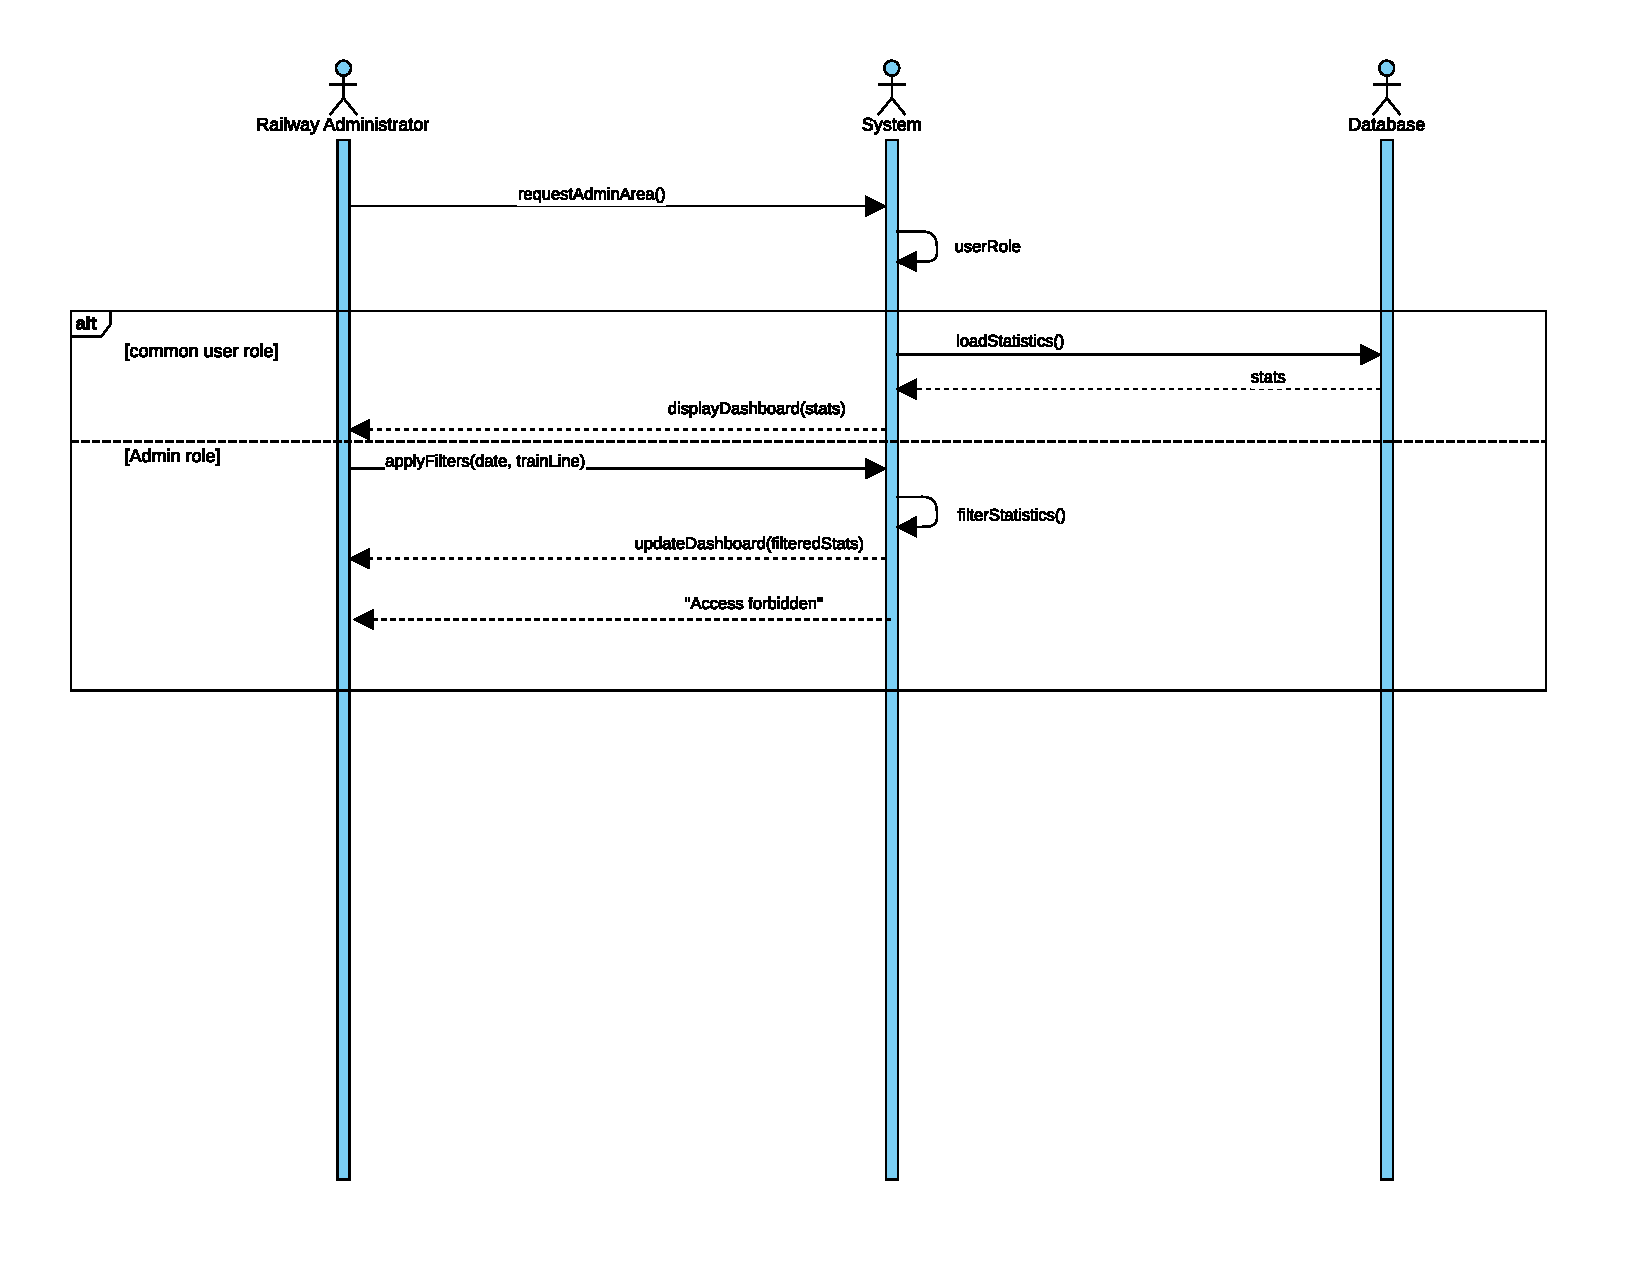
\includegraphics[width=1.3\textwidth]{UC3-sequence diagram.pdf}
\end{figure}
\end{landscape}

\subsection{UC4: Purchase}
%\textbf{Related Functional Requirements:} FR8, FR9, FR10, FR13, FR14, FR21 
\begin{figure}[H]
    \centering
    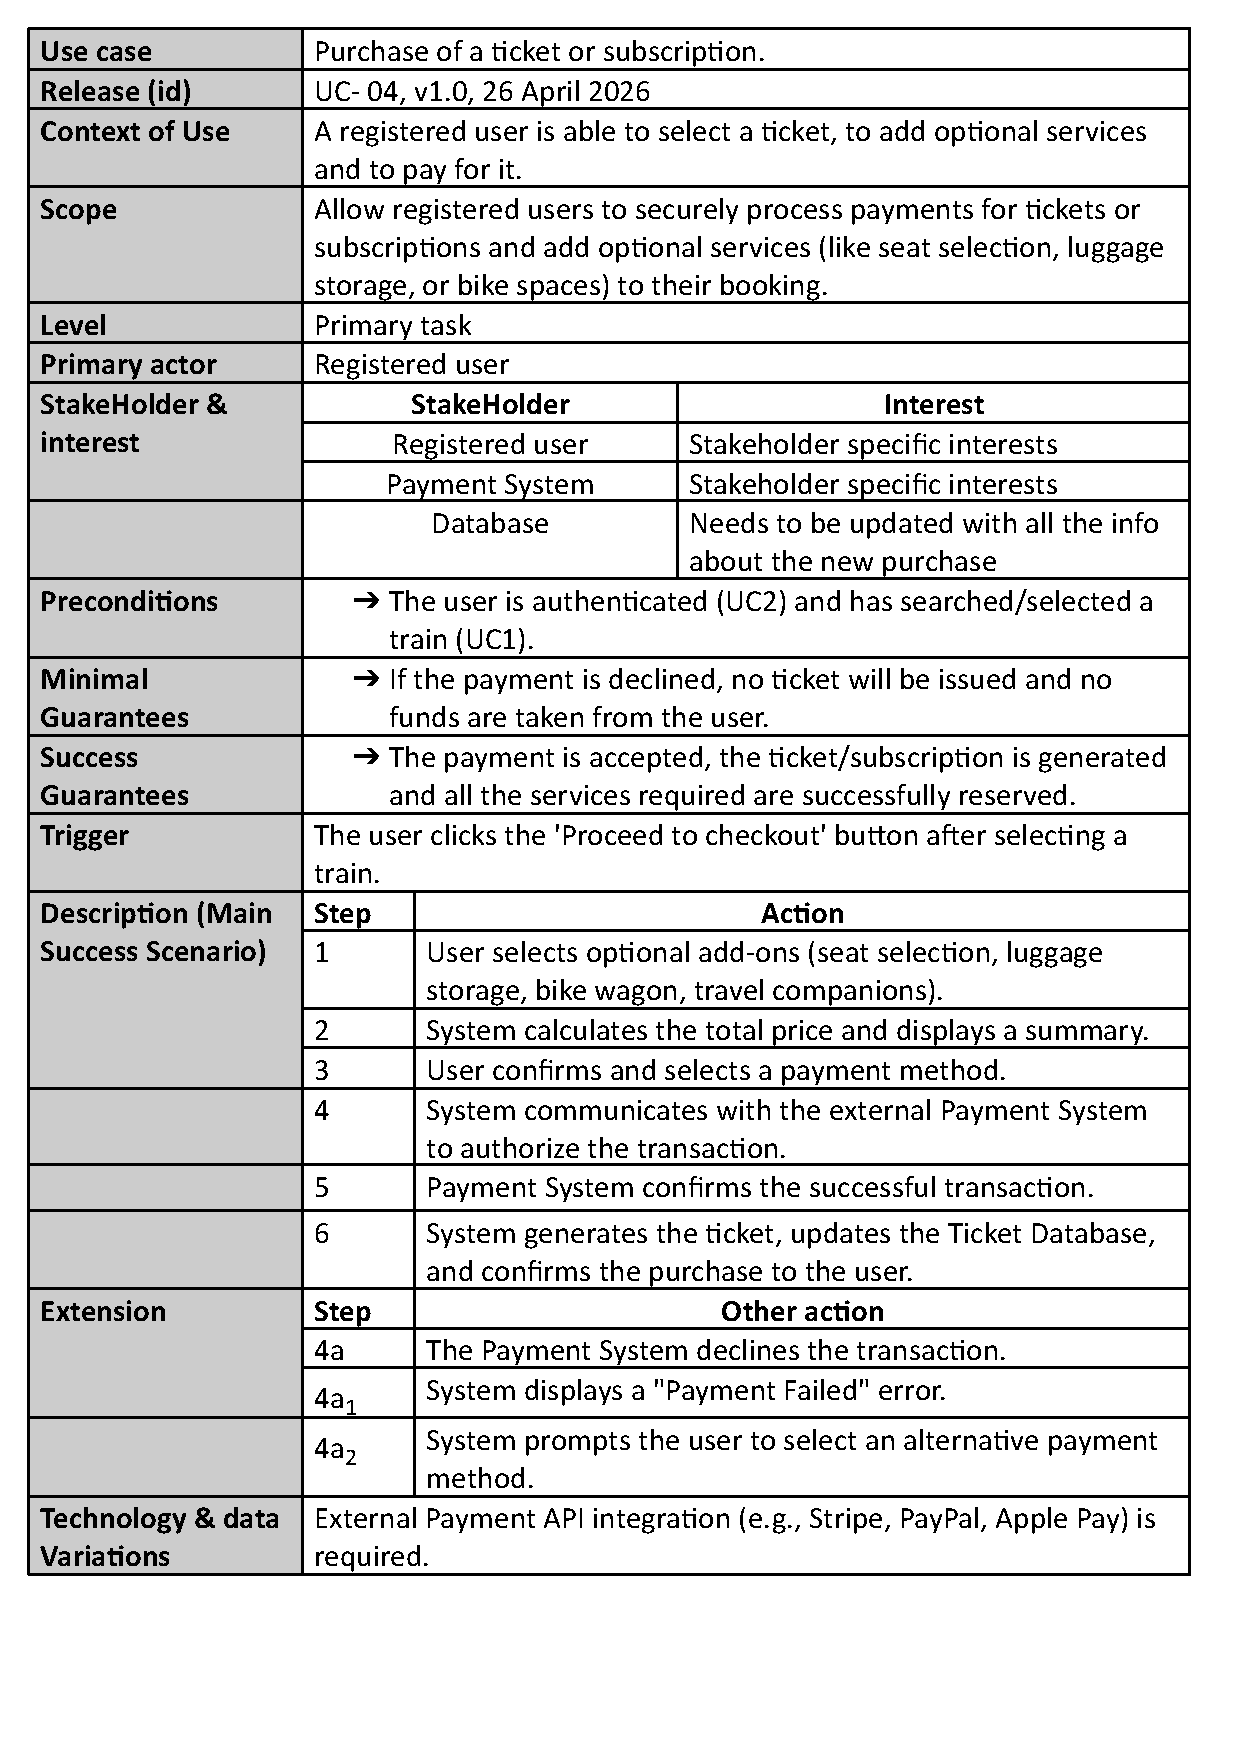
\includegraphics[width=0.9\textwidth]{UC4table.pdf}
\end{figure}
\begin{landscape}
\begin{figure}[H]
    \centering
    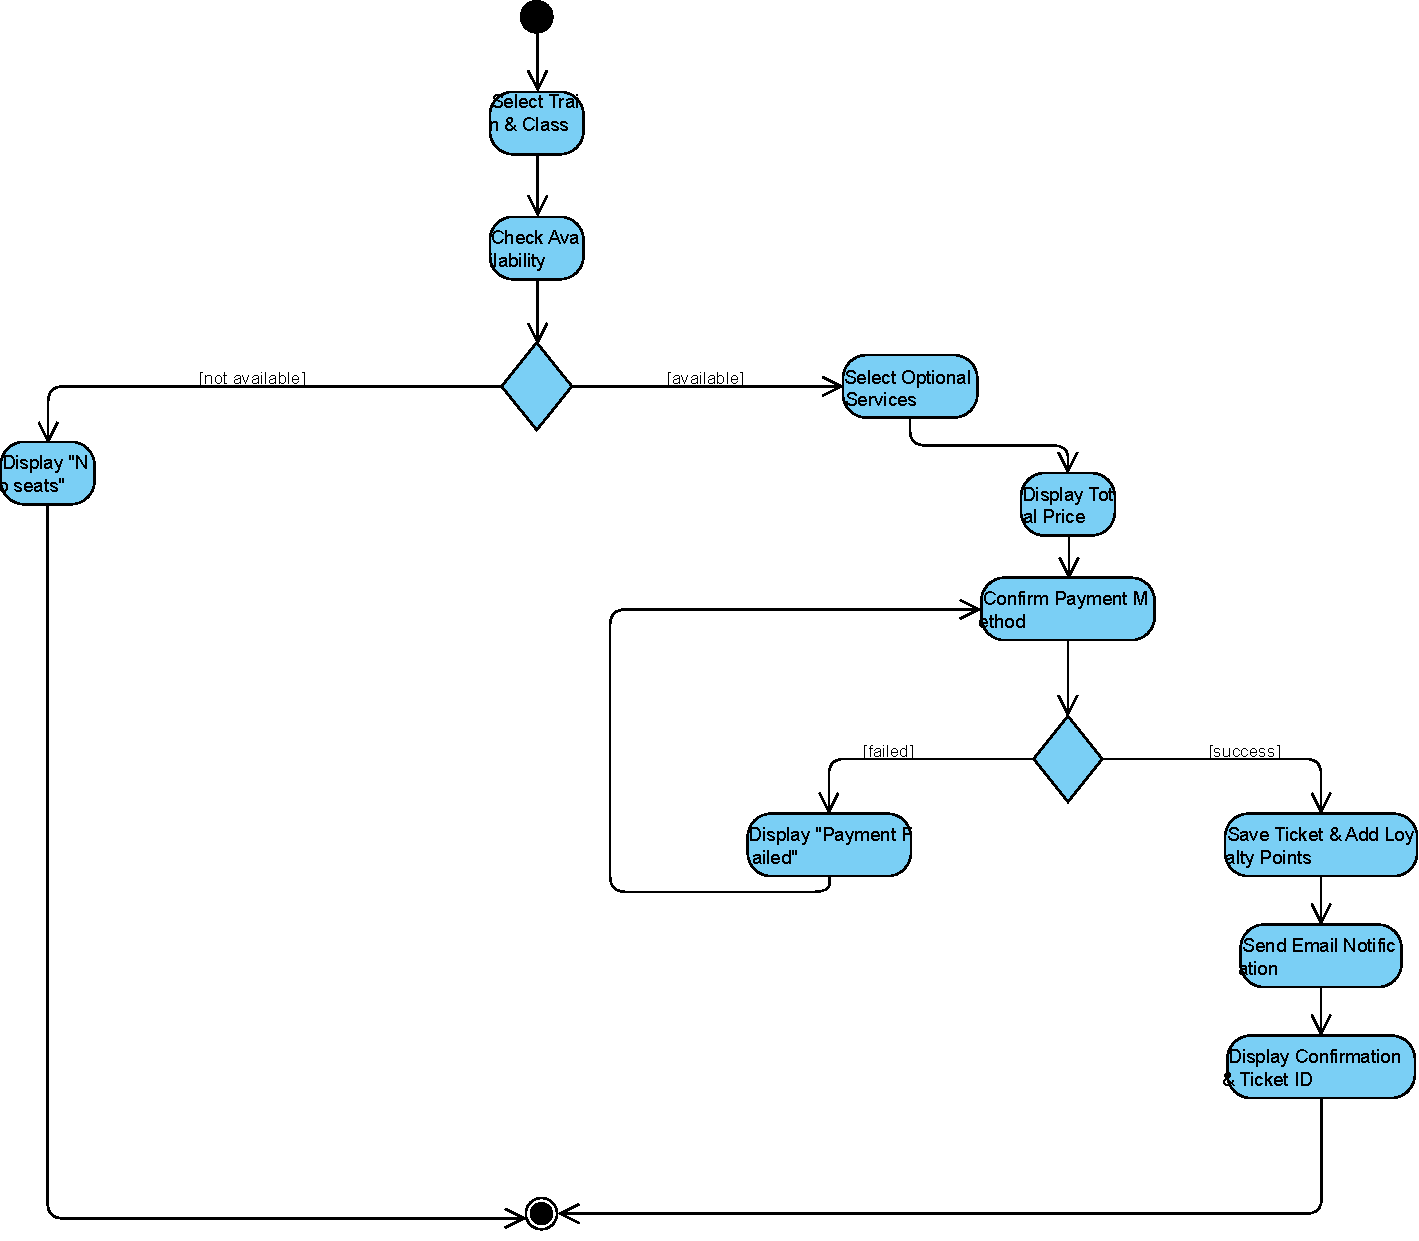
\includegraphics[width=1.0\textwidth]{UC4-activity diagram.pdf}
\end{figure}
\end{landscape}
\begin{landscape}
\begin{figure}[H]
    \centering
    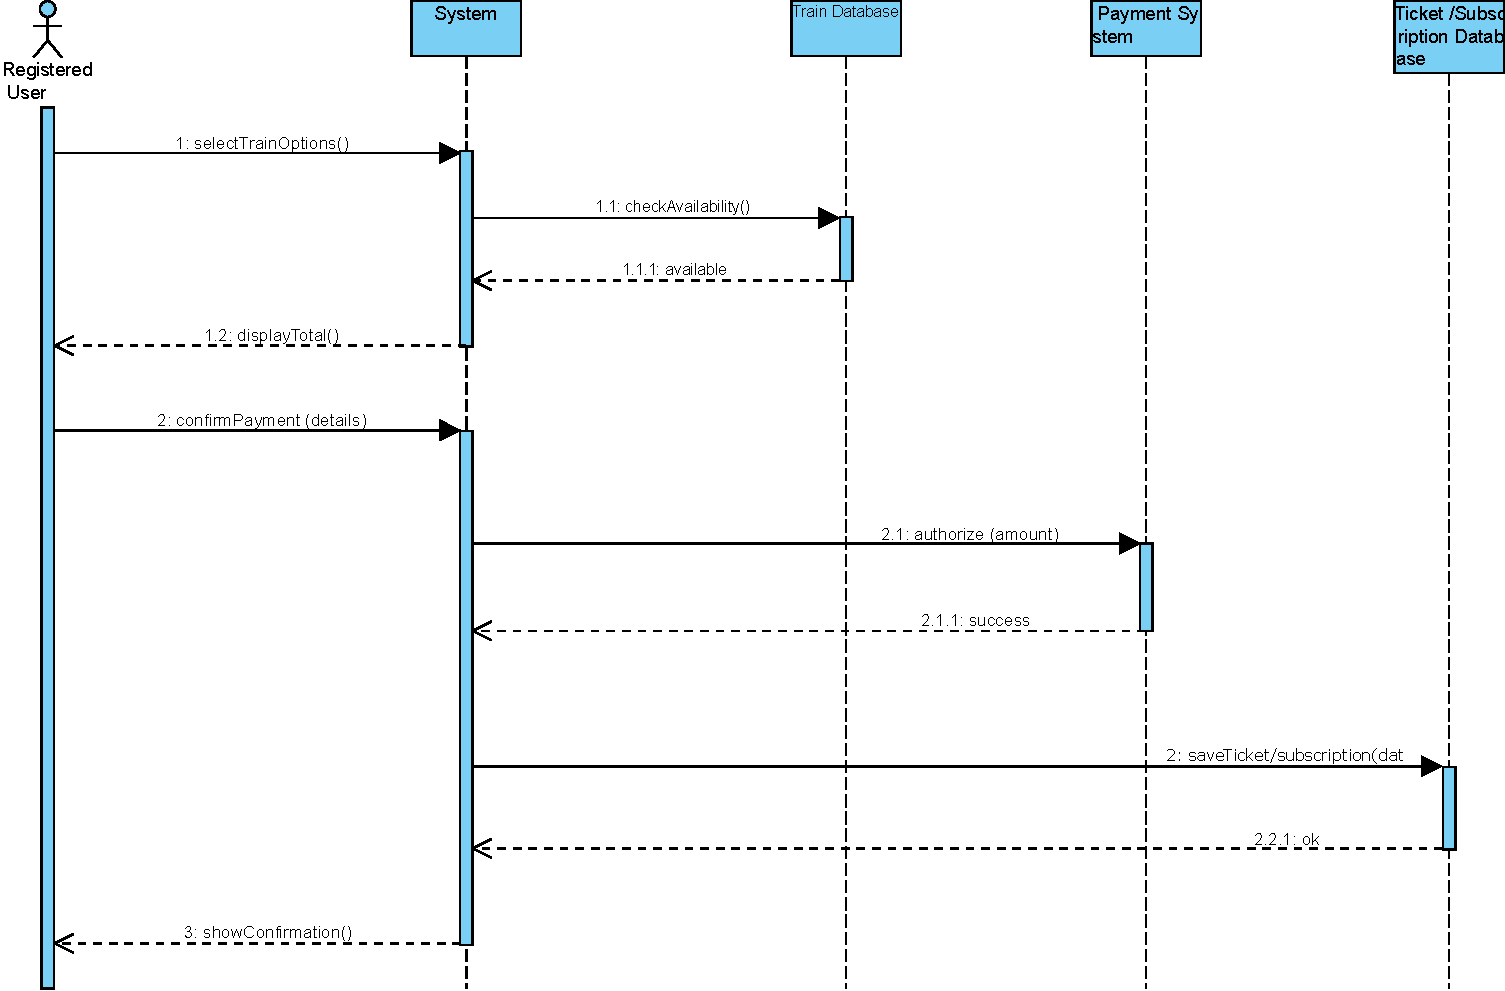
\includegraphics[width=1.4\textwidth]{UC4-sequence diagram.pdf}
\end{figure}
\end{landscape}

\subsection{UC5: Check Train Status}
%\textbf{Related Functional Requirements:} FR15, FR33 
\begin{figure}[H]
    \centering
    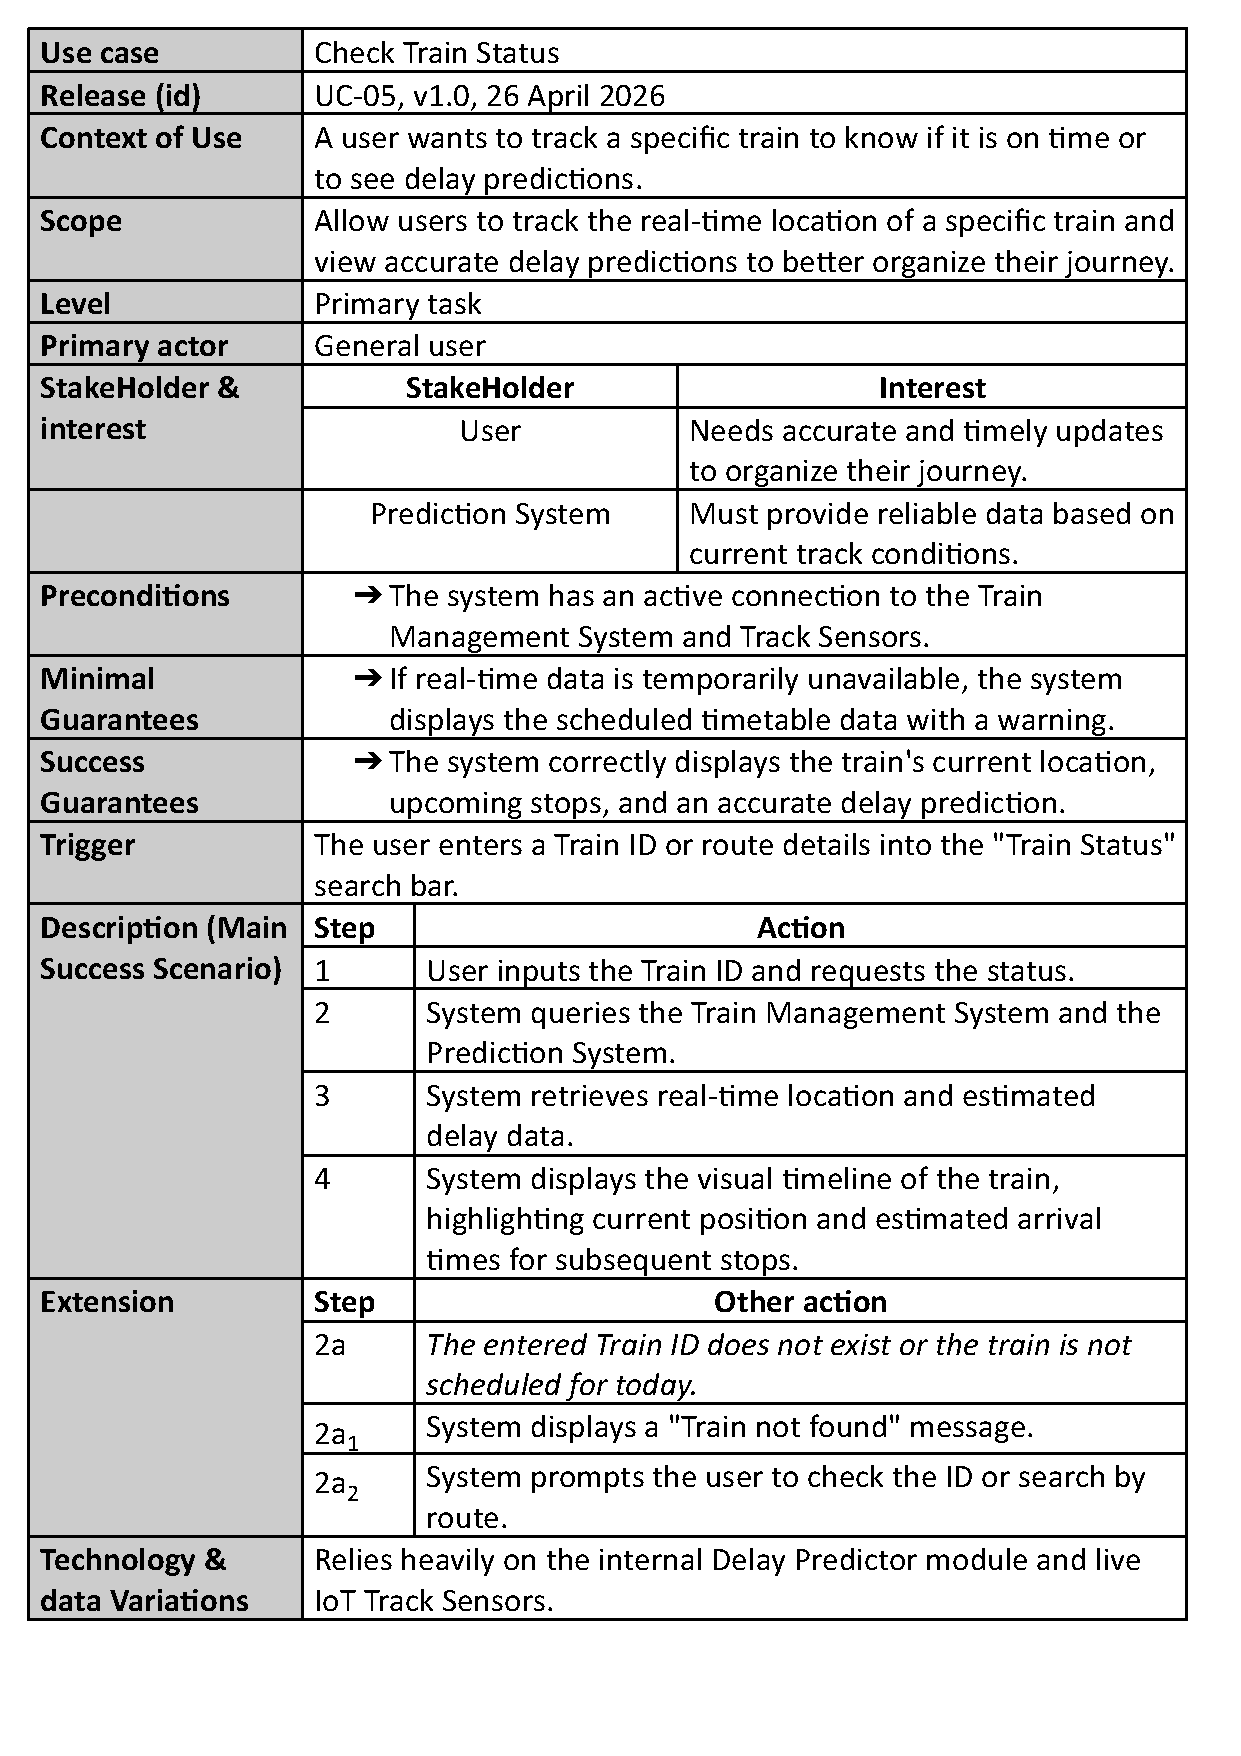
\includegraphics[width=0.9\textwidth]{UC5table.pdf}
\end{figure}
\begin{landscape}
\begin{figure}[H]
    \centering
    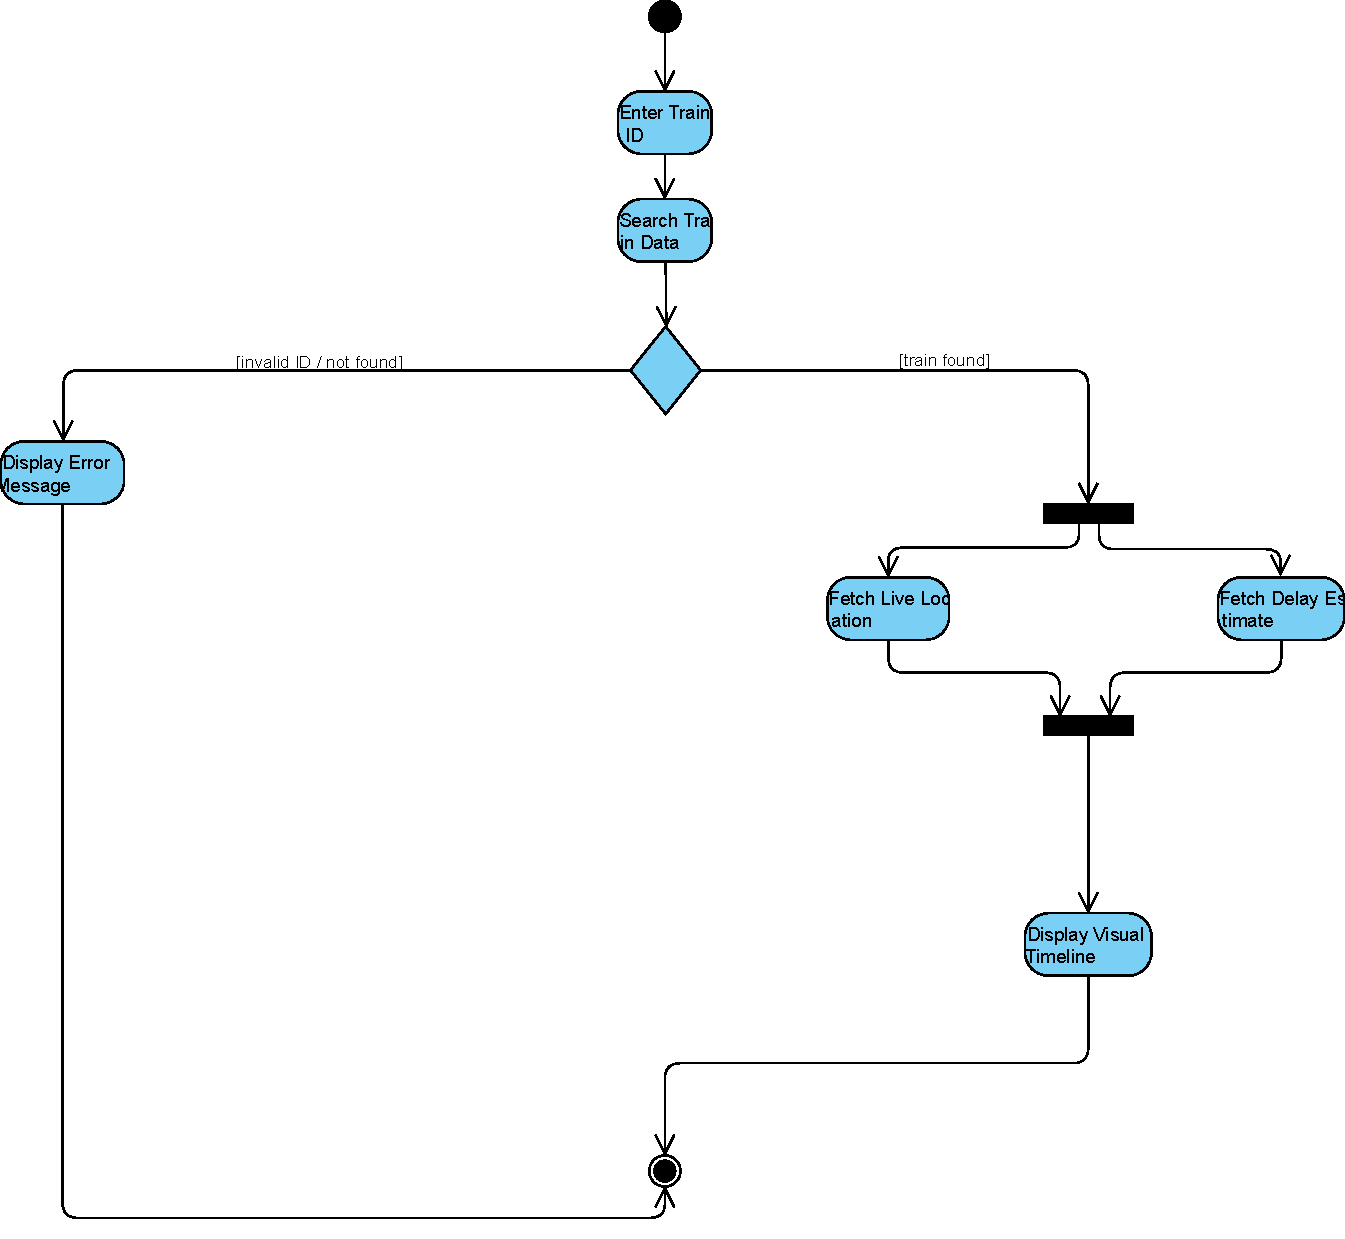
\includegraphics[width=1.0\textwidth]{UC5-activity diagram.pdf}
\end{figure}
\end{landscape}
\begin{landscape}
\begin{figure}[H]
    \centering
    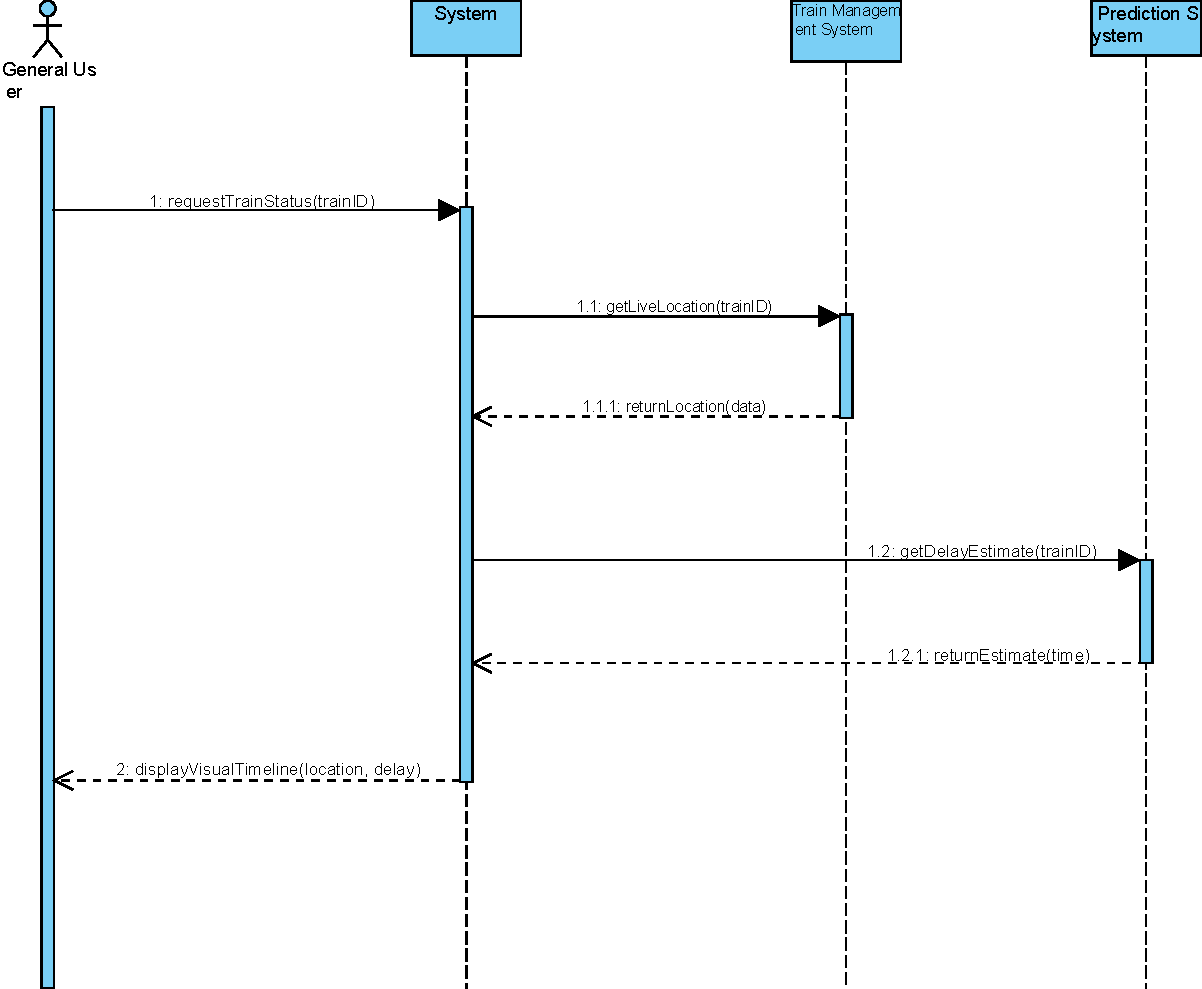
\includegraphics[width=1.2\textwidth]{UC5-sequence diagram.pdf}
\end{figure}
\end{landscape}

\subsection{UC6: Boards Visualization}
%\textbf{Related Functional Requirements:} FR6 
\begin{figure}[H]
    \centering
    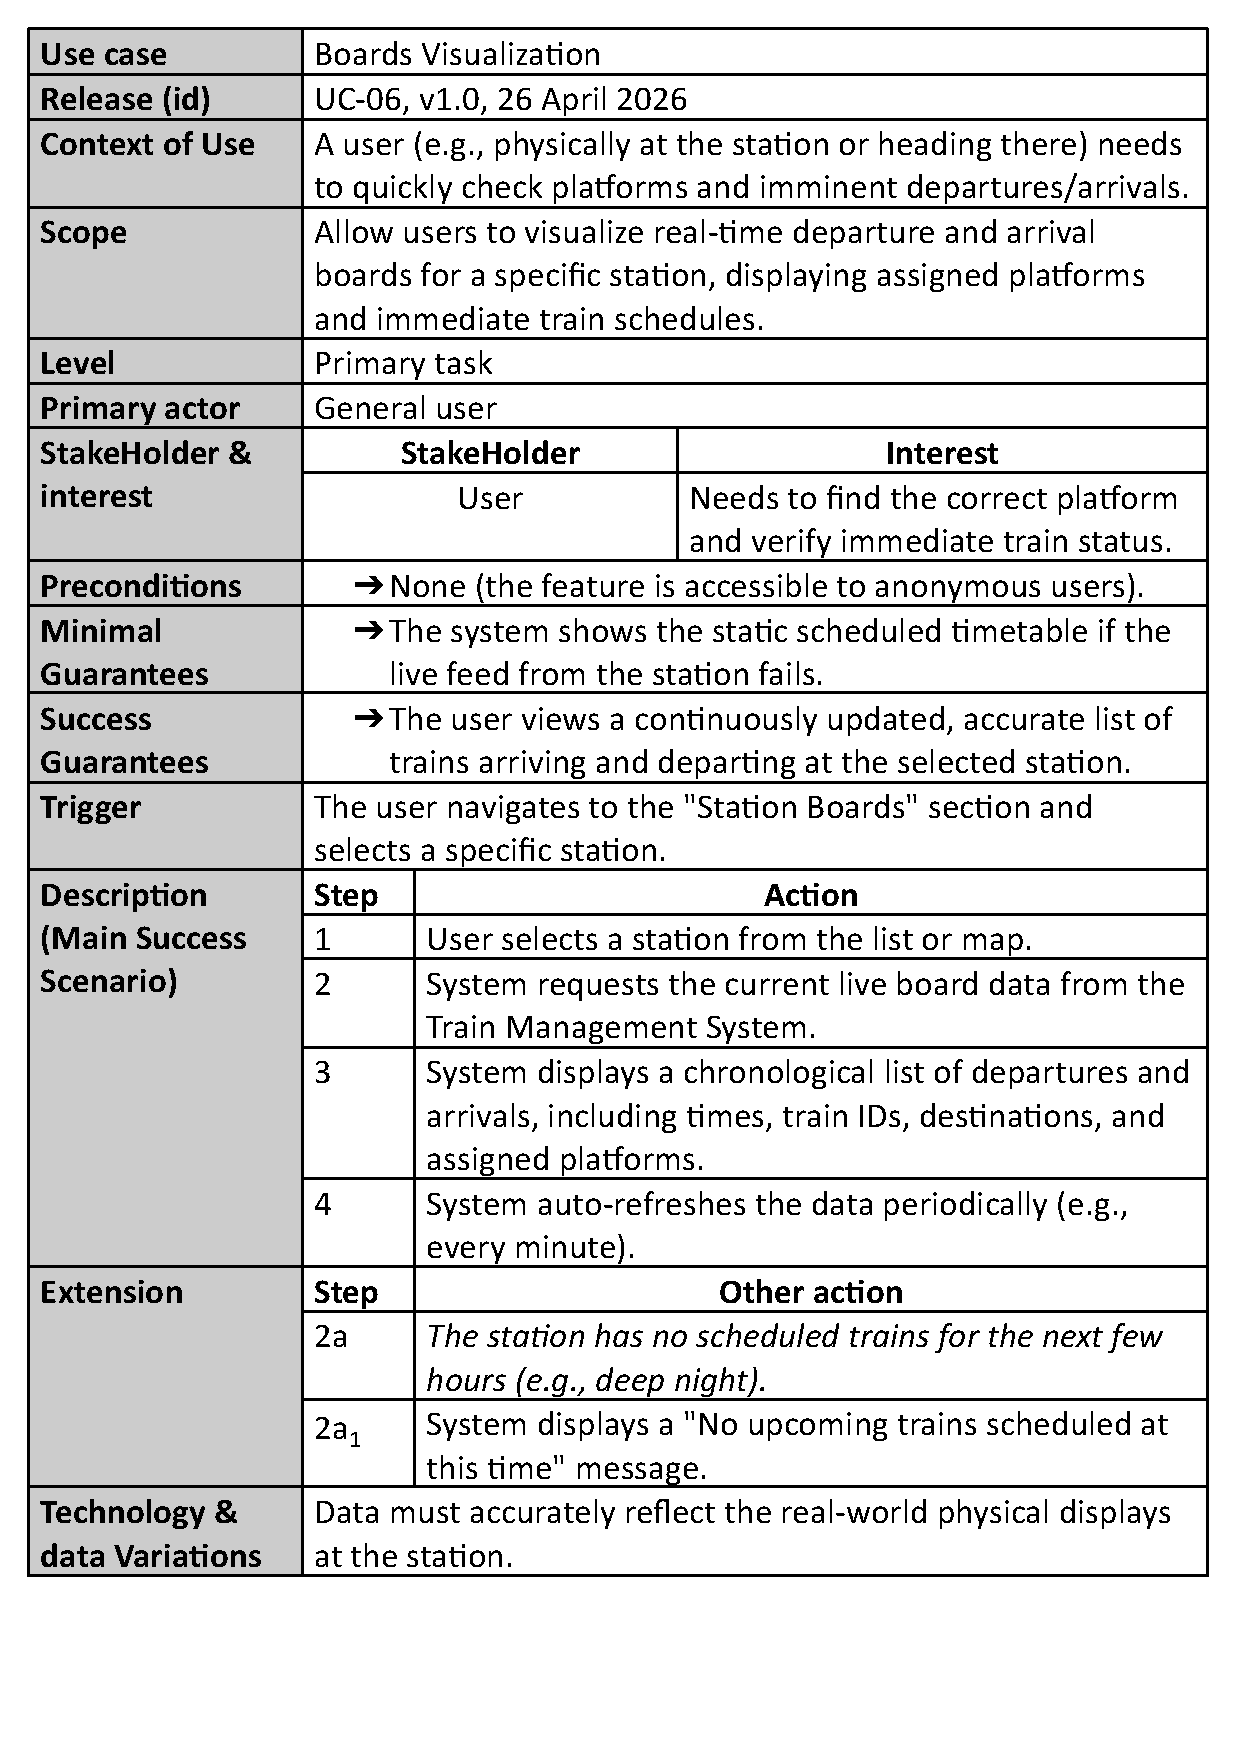
\includegraphics[width=0.9\textwidth]{UC6table.pdf}
\end{figure}
\begin{landscape}
\begin{figure}[H]
    \centering
    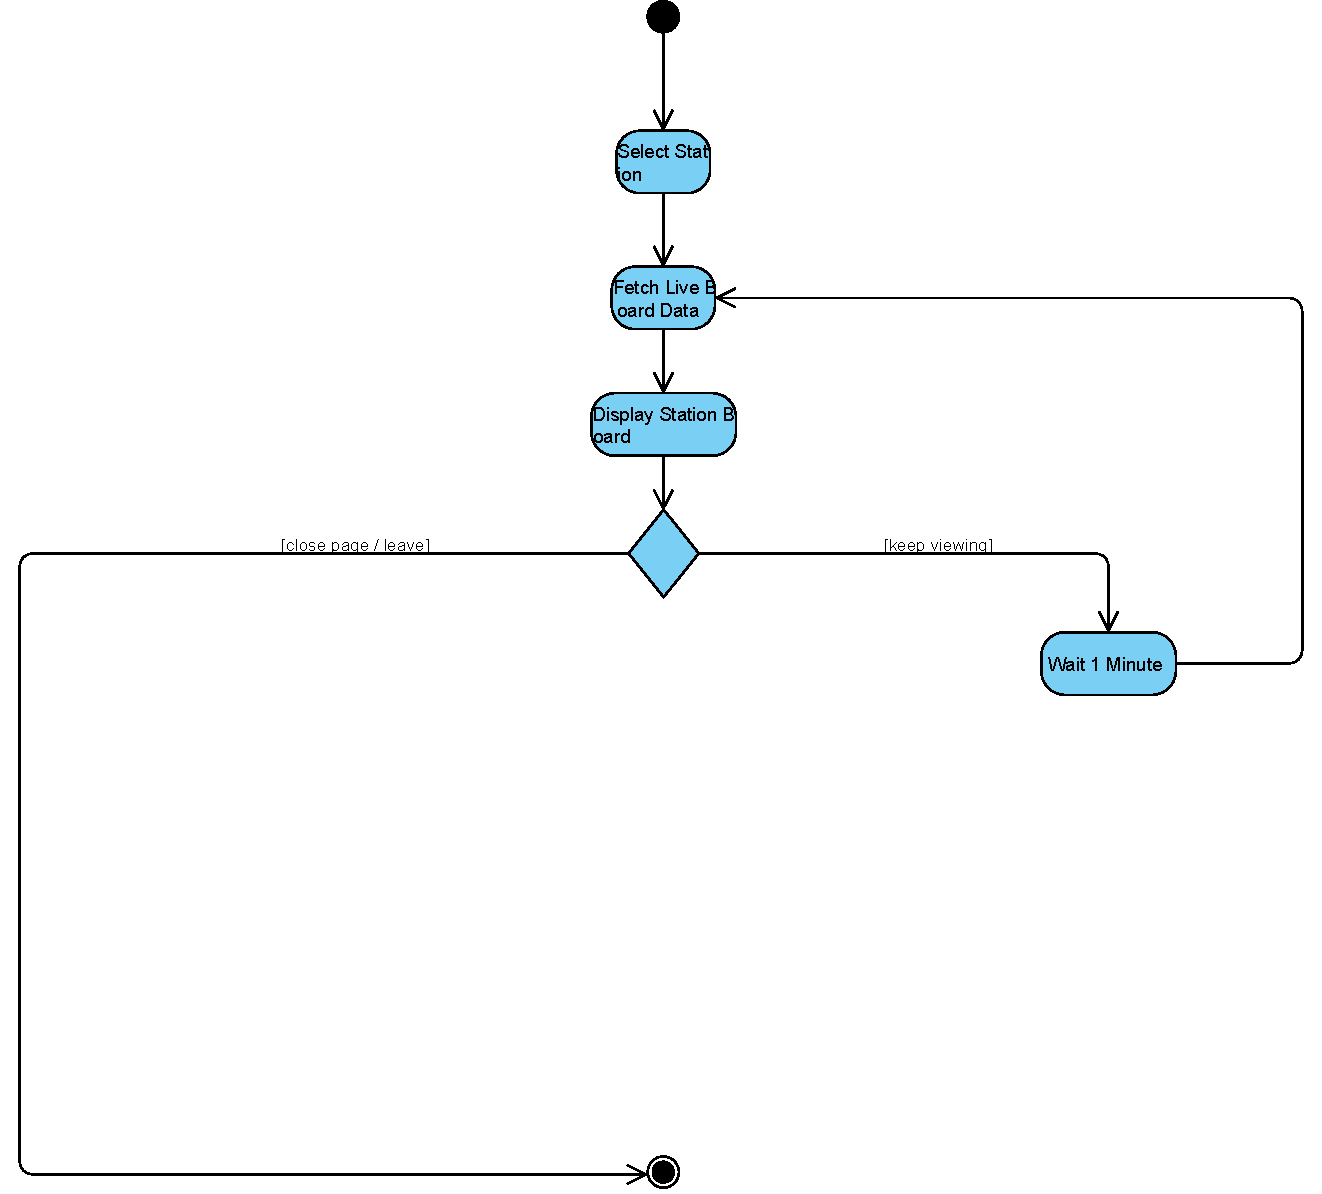
\includegraphics[width=1.0\textwidth]{UC6-activity diagram.pdf}
\end{figure}
\begin{figure}[H]
    \centering
    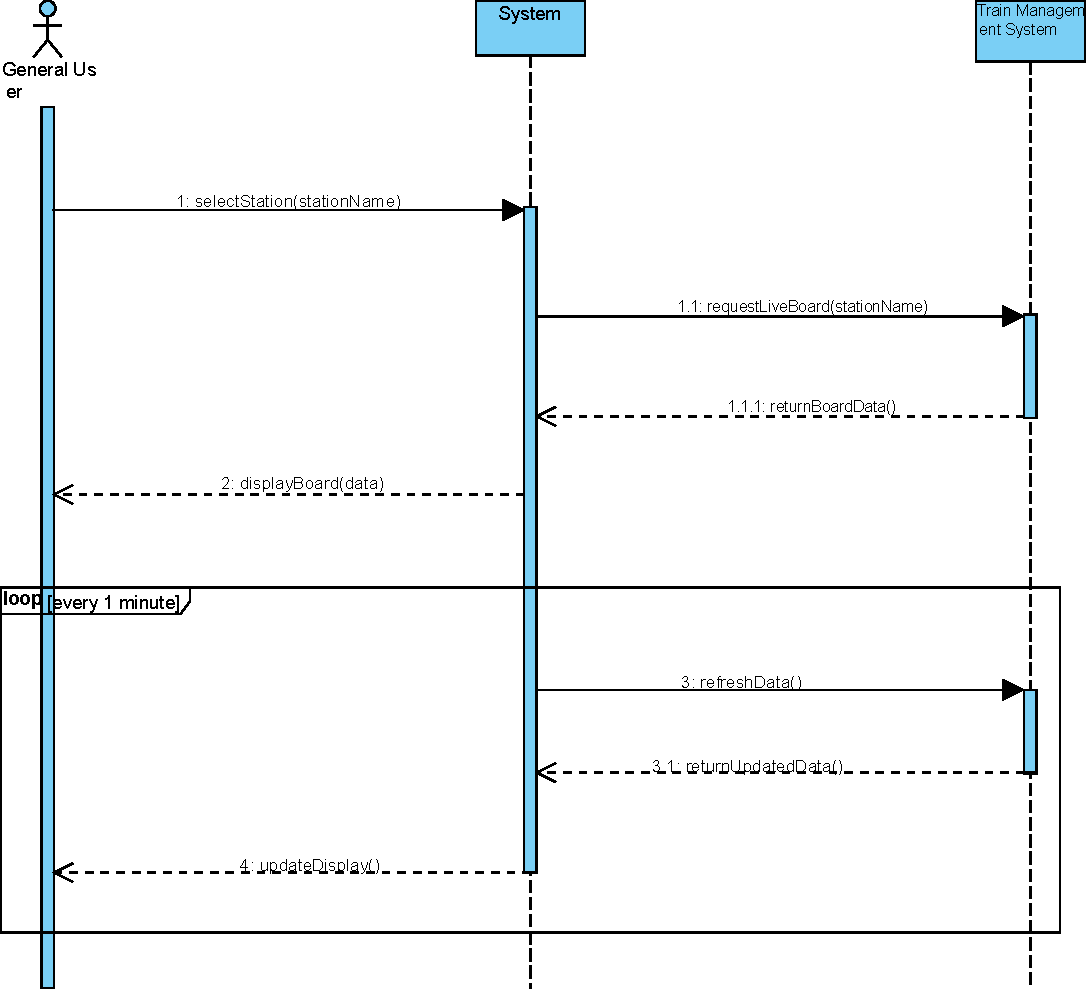
\includegraphics[width=1.1\textwidth]{UC6-sequence diagram.pdf}
\end{figure}
\end{landscape}

\subsection{UC7: Receive Notifications}
%\textbf{Related Functional Requirements:} FR23 
\begin{figure}[H]
    \centering
    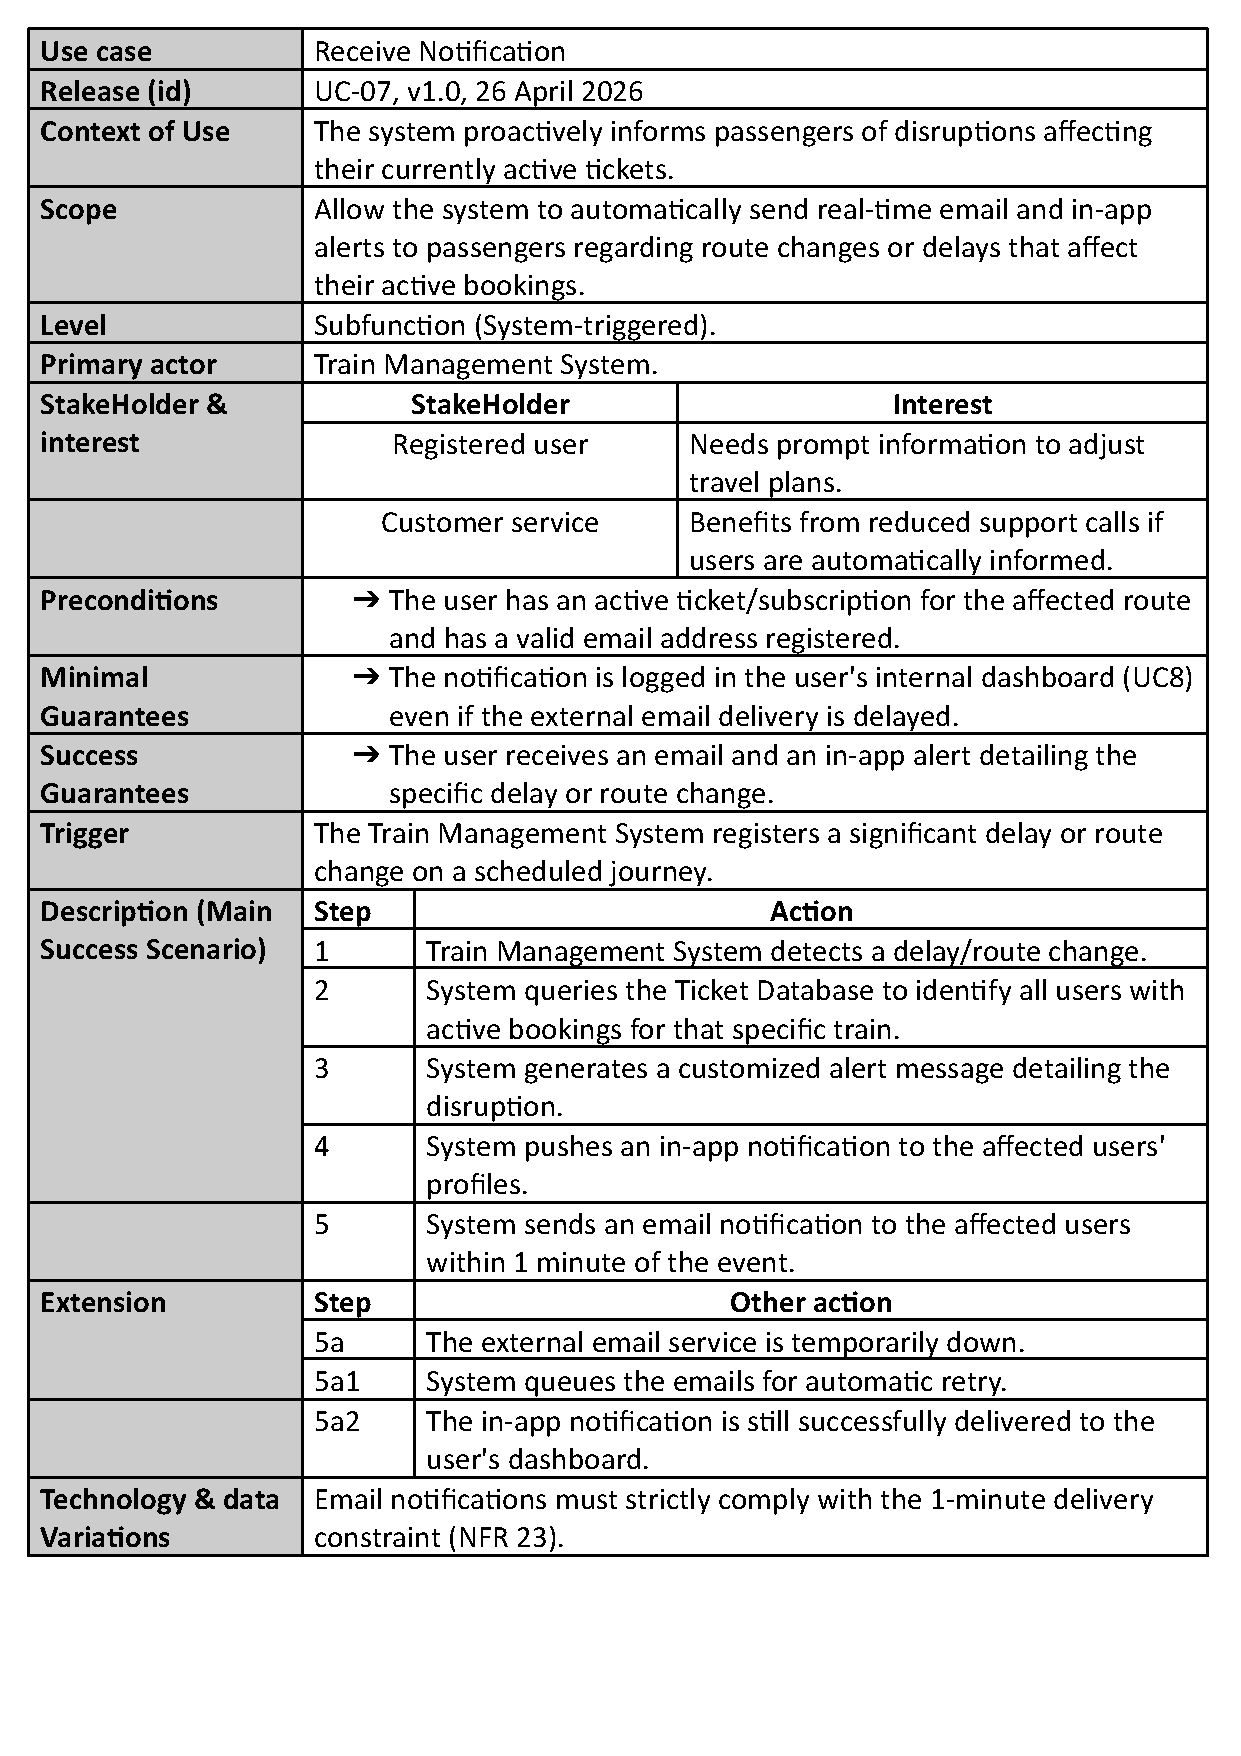
\includegraphics[width=0.9\textwidth]{UC7table.pdf}
\end{figure}
\begin{landscape}
\begin{figure}[H]
    \centering
    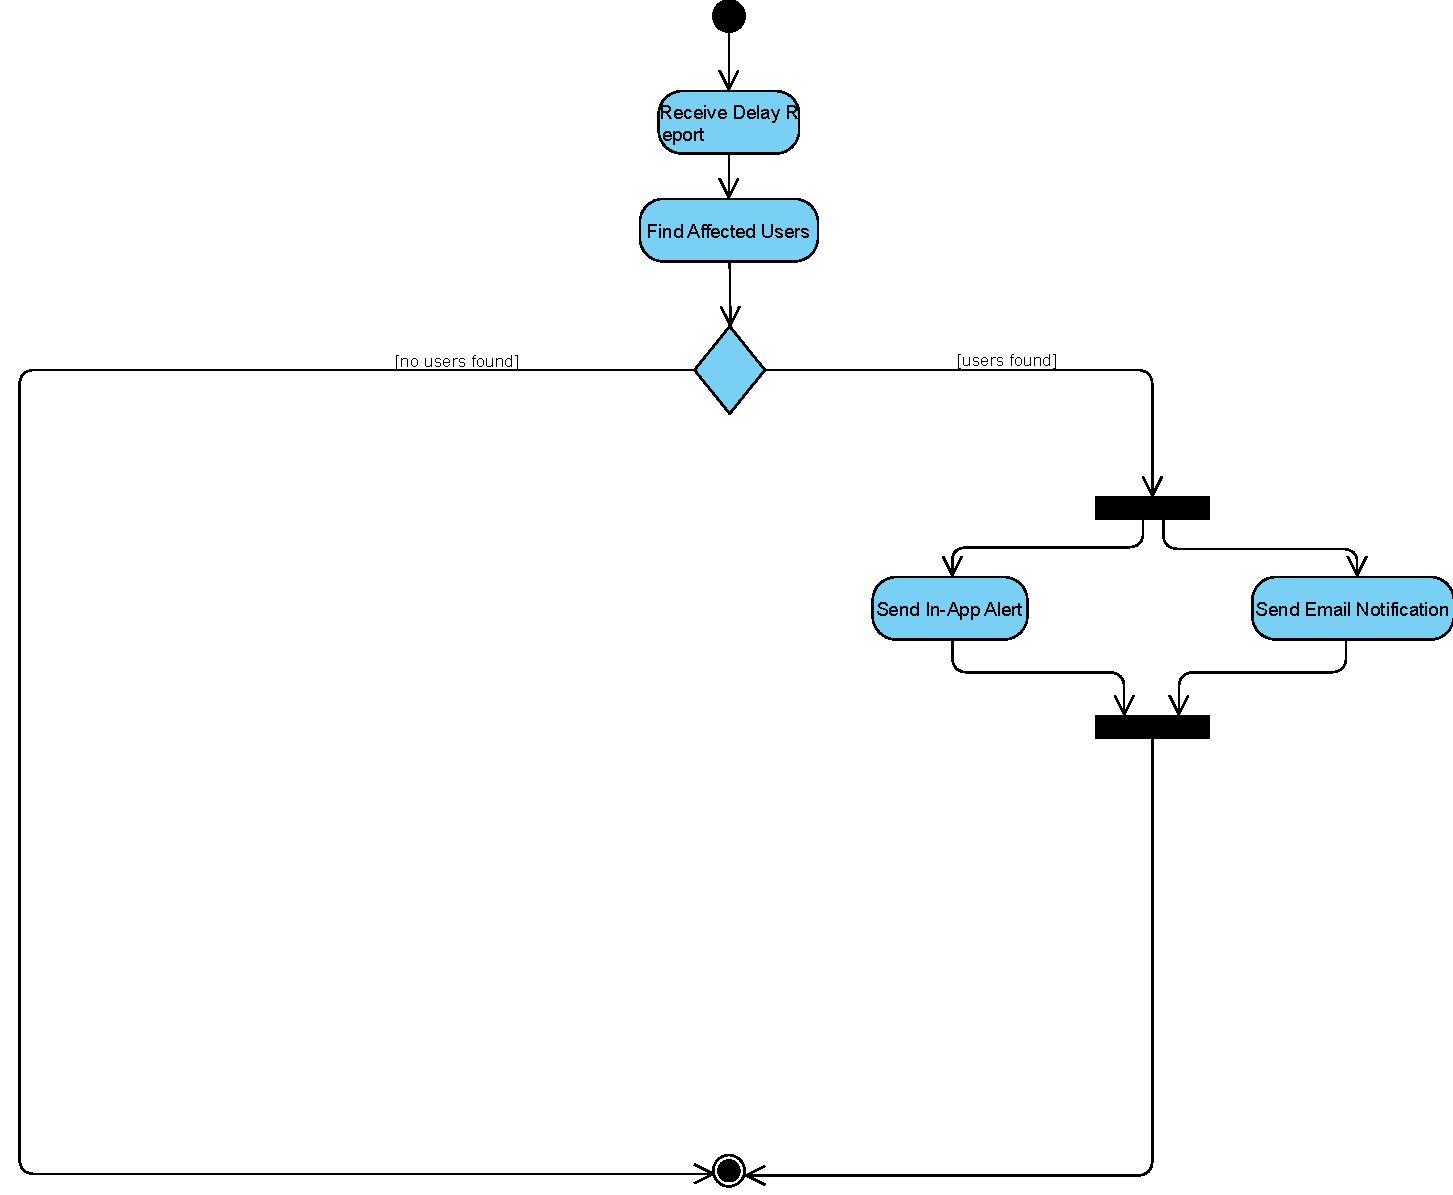
\includegraphics[width=1.0\textwidth]{UC7-activity diagram.pdf}
\end{figure}
\begin{figure}[H]
    \centering
    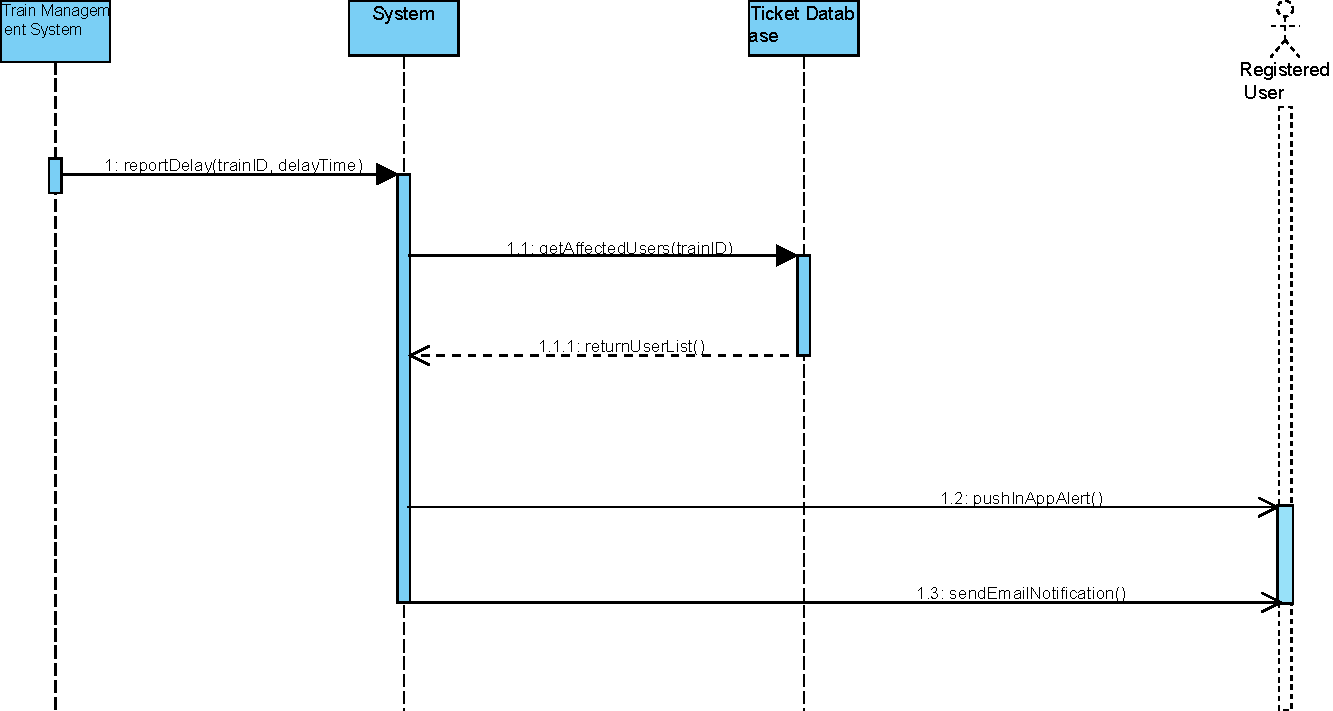
\includegraphics[width=1.3\textwidth]{UC7-sequence diagram.pdf}
\end{figure}
\end{landscape}

\subsection{UC8: User Dashboard / Profile}
%\textbf{Related Functional Requirements:} FR17, FR18, FR19, FR20 
\begin{figure}[H]
    \centering
    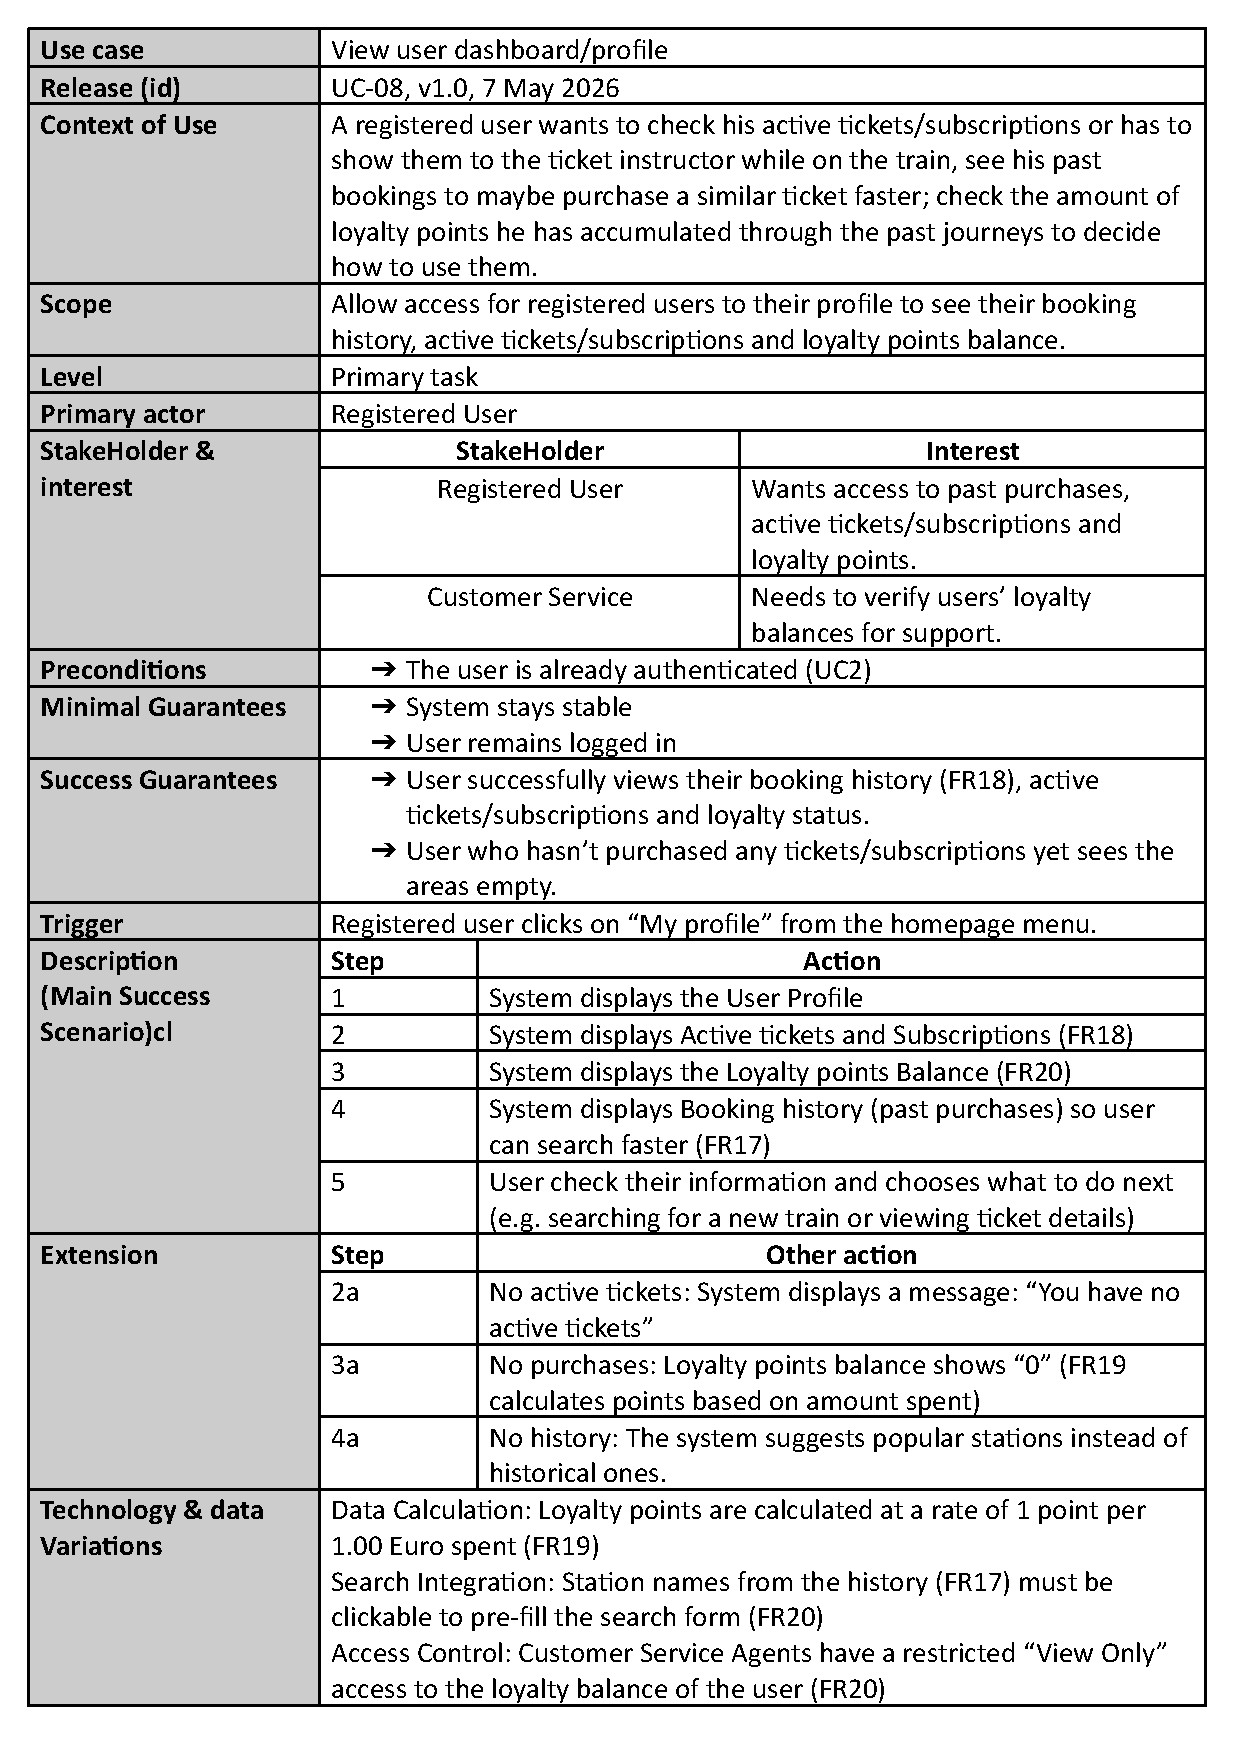
\includegraphics[width=0.9\textwidth]{UC8table.pdf}
\end{figure}
\begin{figure}[H]
    \centering
    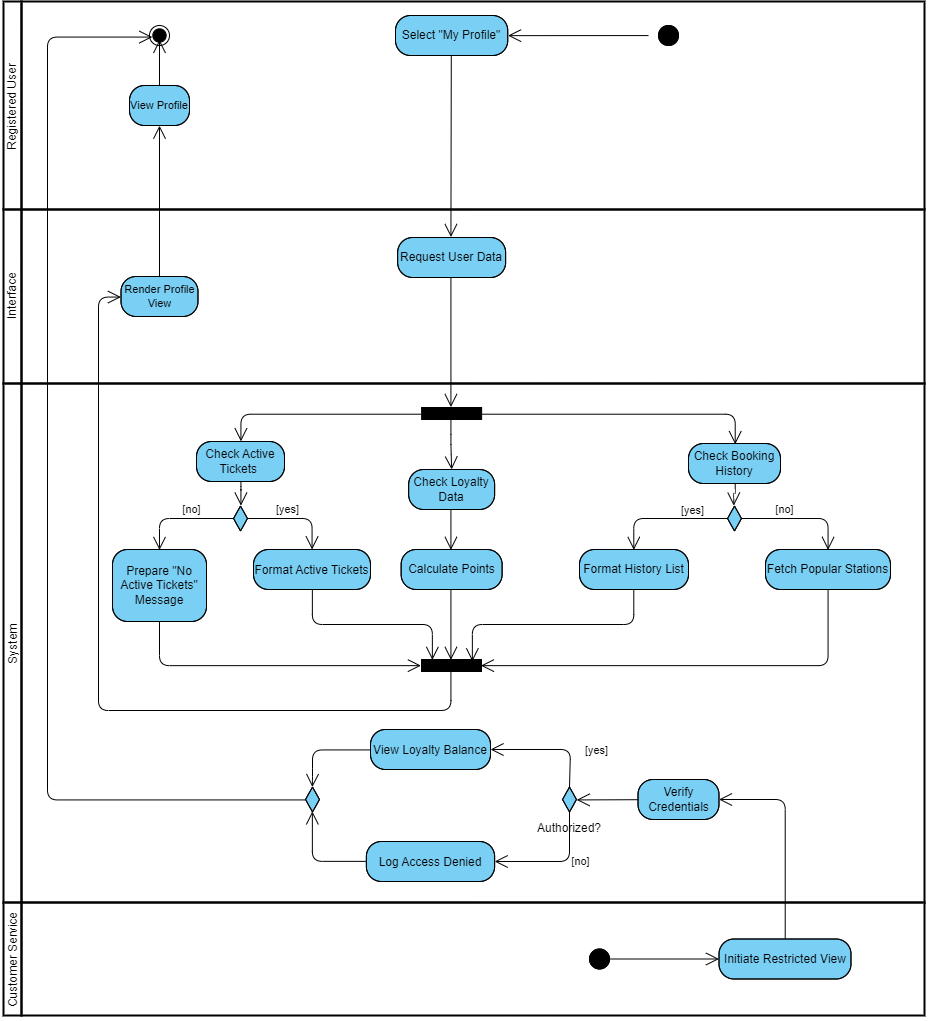
\includegraphics[width=1.0\textwidth]{UC8-activity diagram.png}
\end{figure}
\begin{landscape}
\begin{figure}[H]
    \centering
    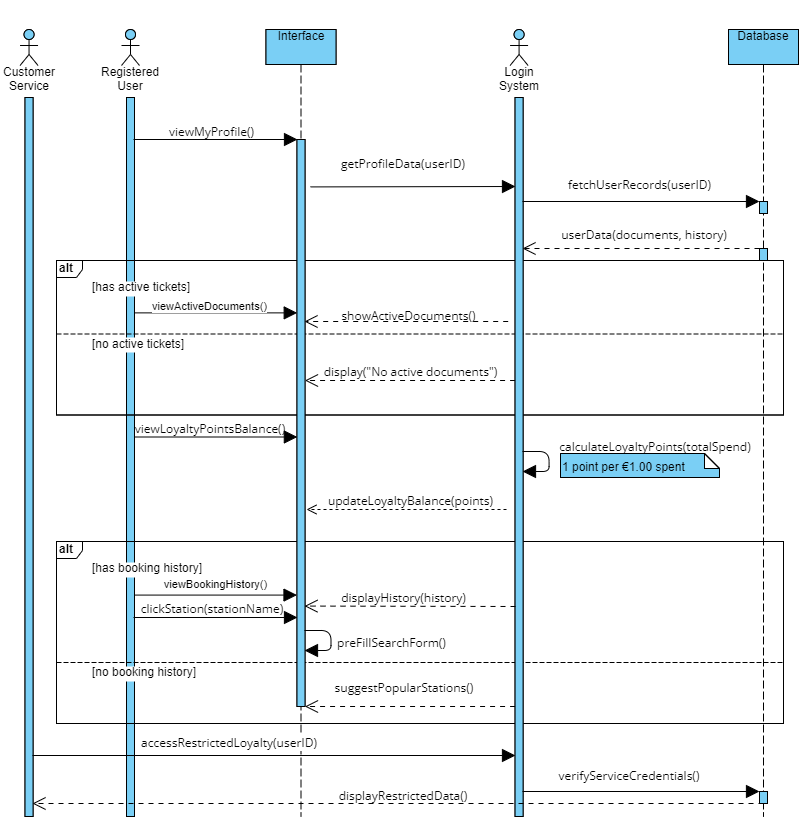
\includegraphics[width=0.9\textwidth]{UC8-sequence diagram.png}
\end{figure}
\end{landscape}

\subsection{UC9: Ticket Management}
%\textbf{Related Functional Requirements:} FR16 
\begin{figure}[H]
    \centering
    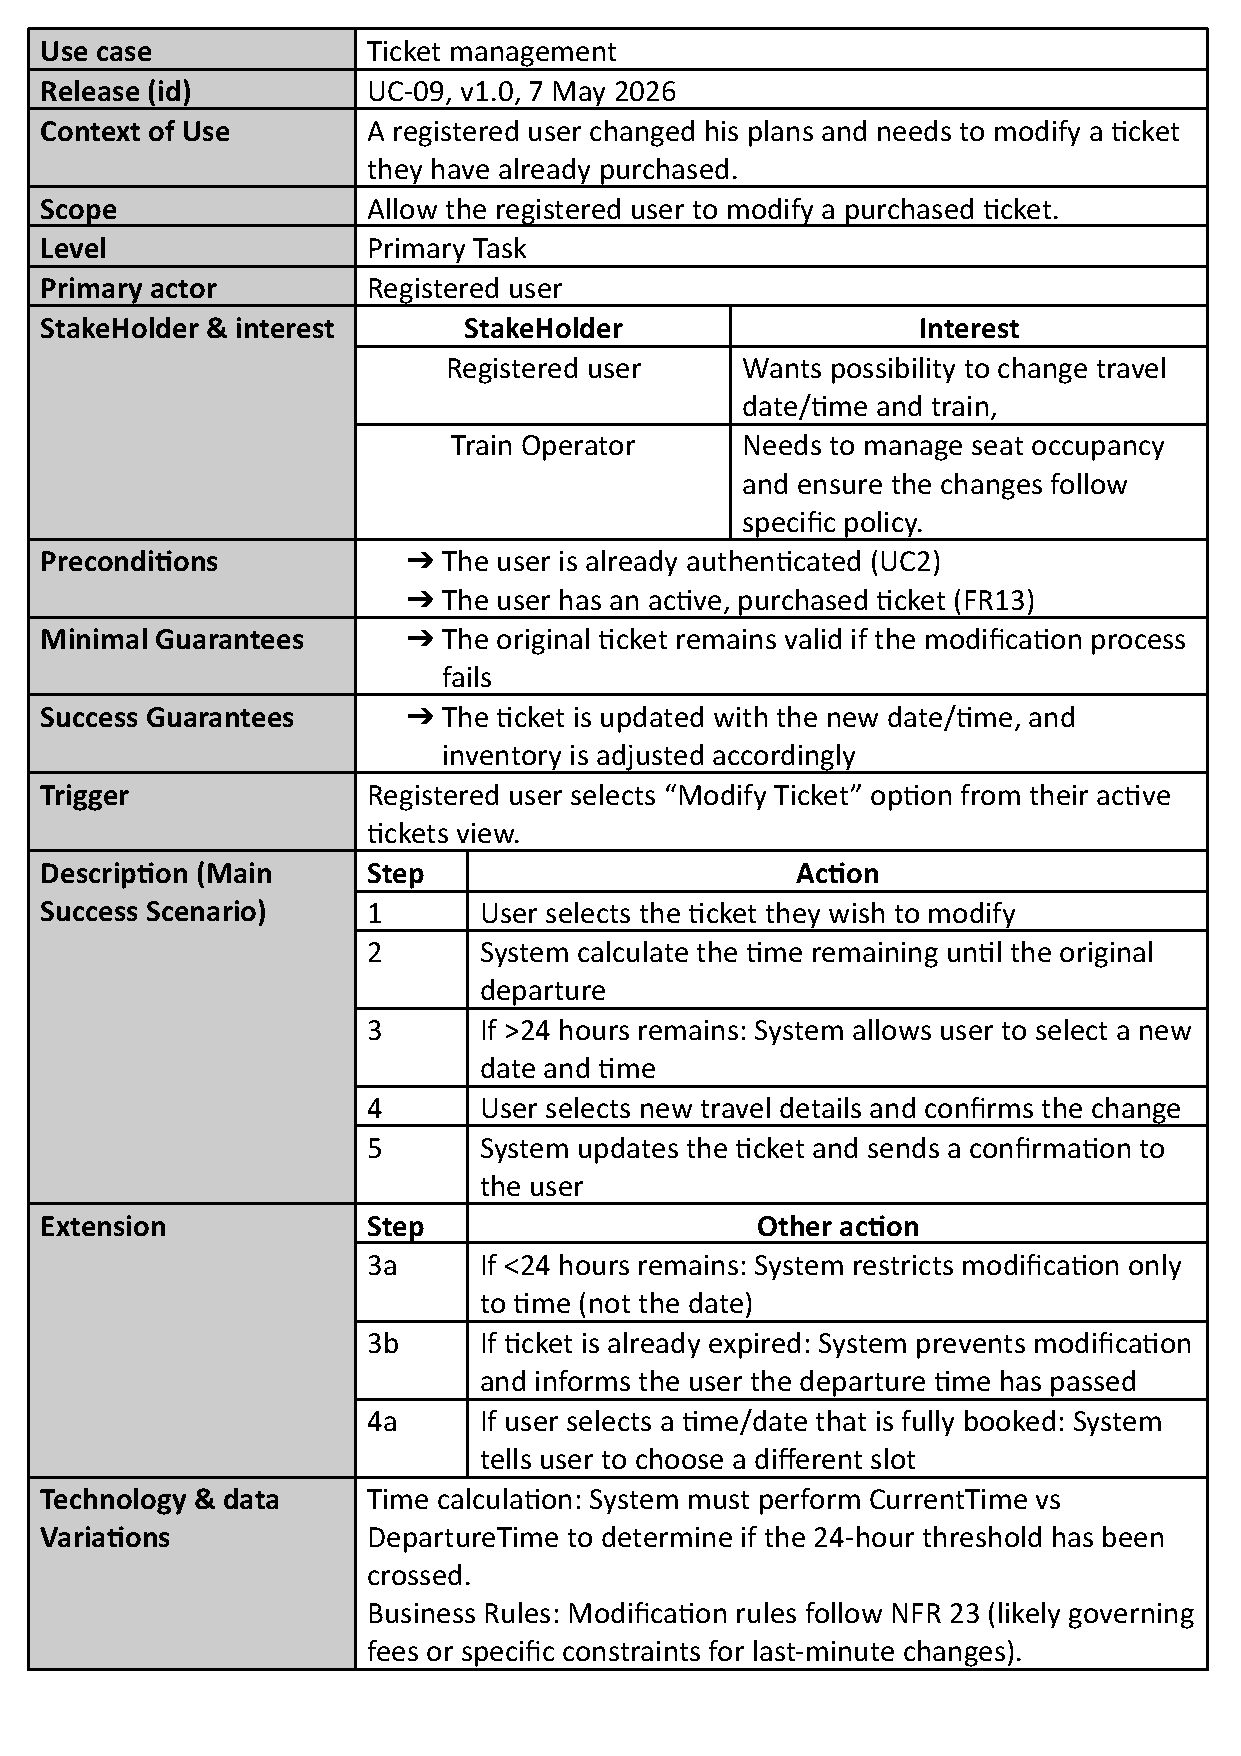
\includegraphics[width=0.9\textwidth]{UC9table.pdf}
\end{figure}
\begin{landscape}
\begin{figure}[H]
    \centering
    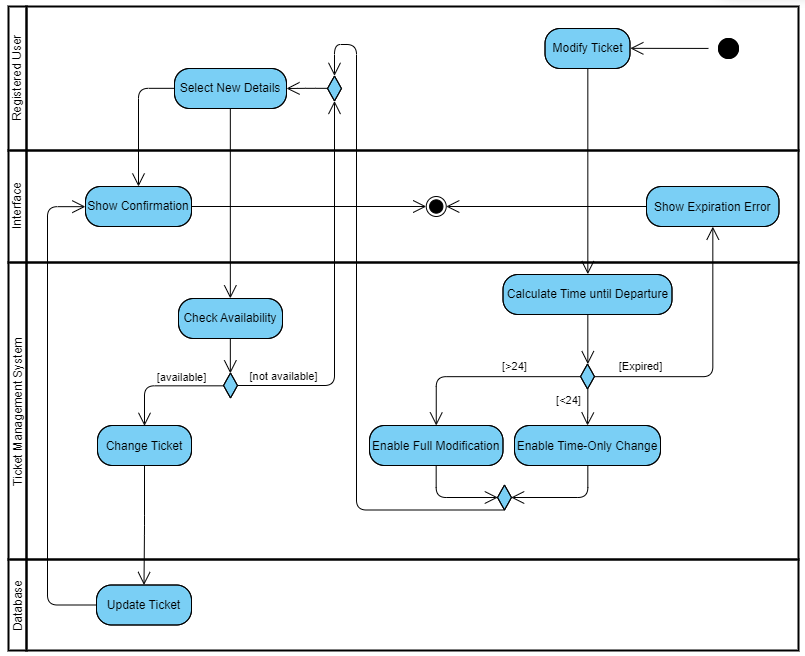
\includegraphics[width=1.1\textwidth]{UC9-activity diagram.png}
\end{figure}
\end{landscape}
\begin{landscape}
\begin{figure}[H]
    \centering
    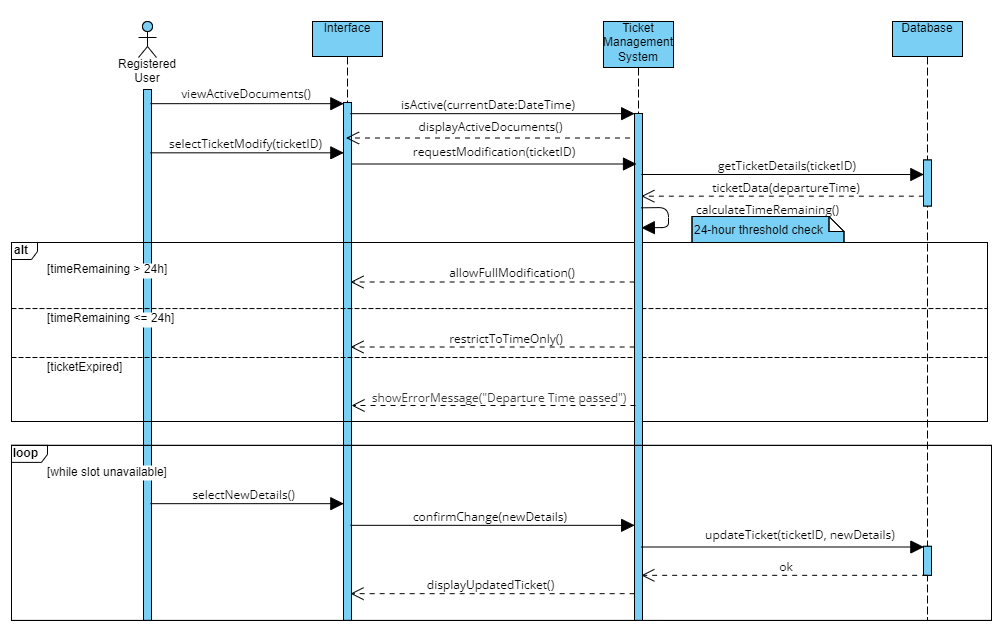
\includegraphics[width=1.2\textwidth]{UC9-sequence diagram.png}
\end{figure}
\end{landscape}

\subsection{UC10: Account Management}
%\textbf{Related Functional Requirements:} FR27, FR29, FR30 
\begin{figure}[H]
    \centering
    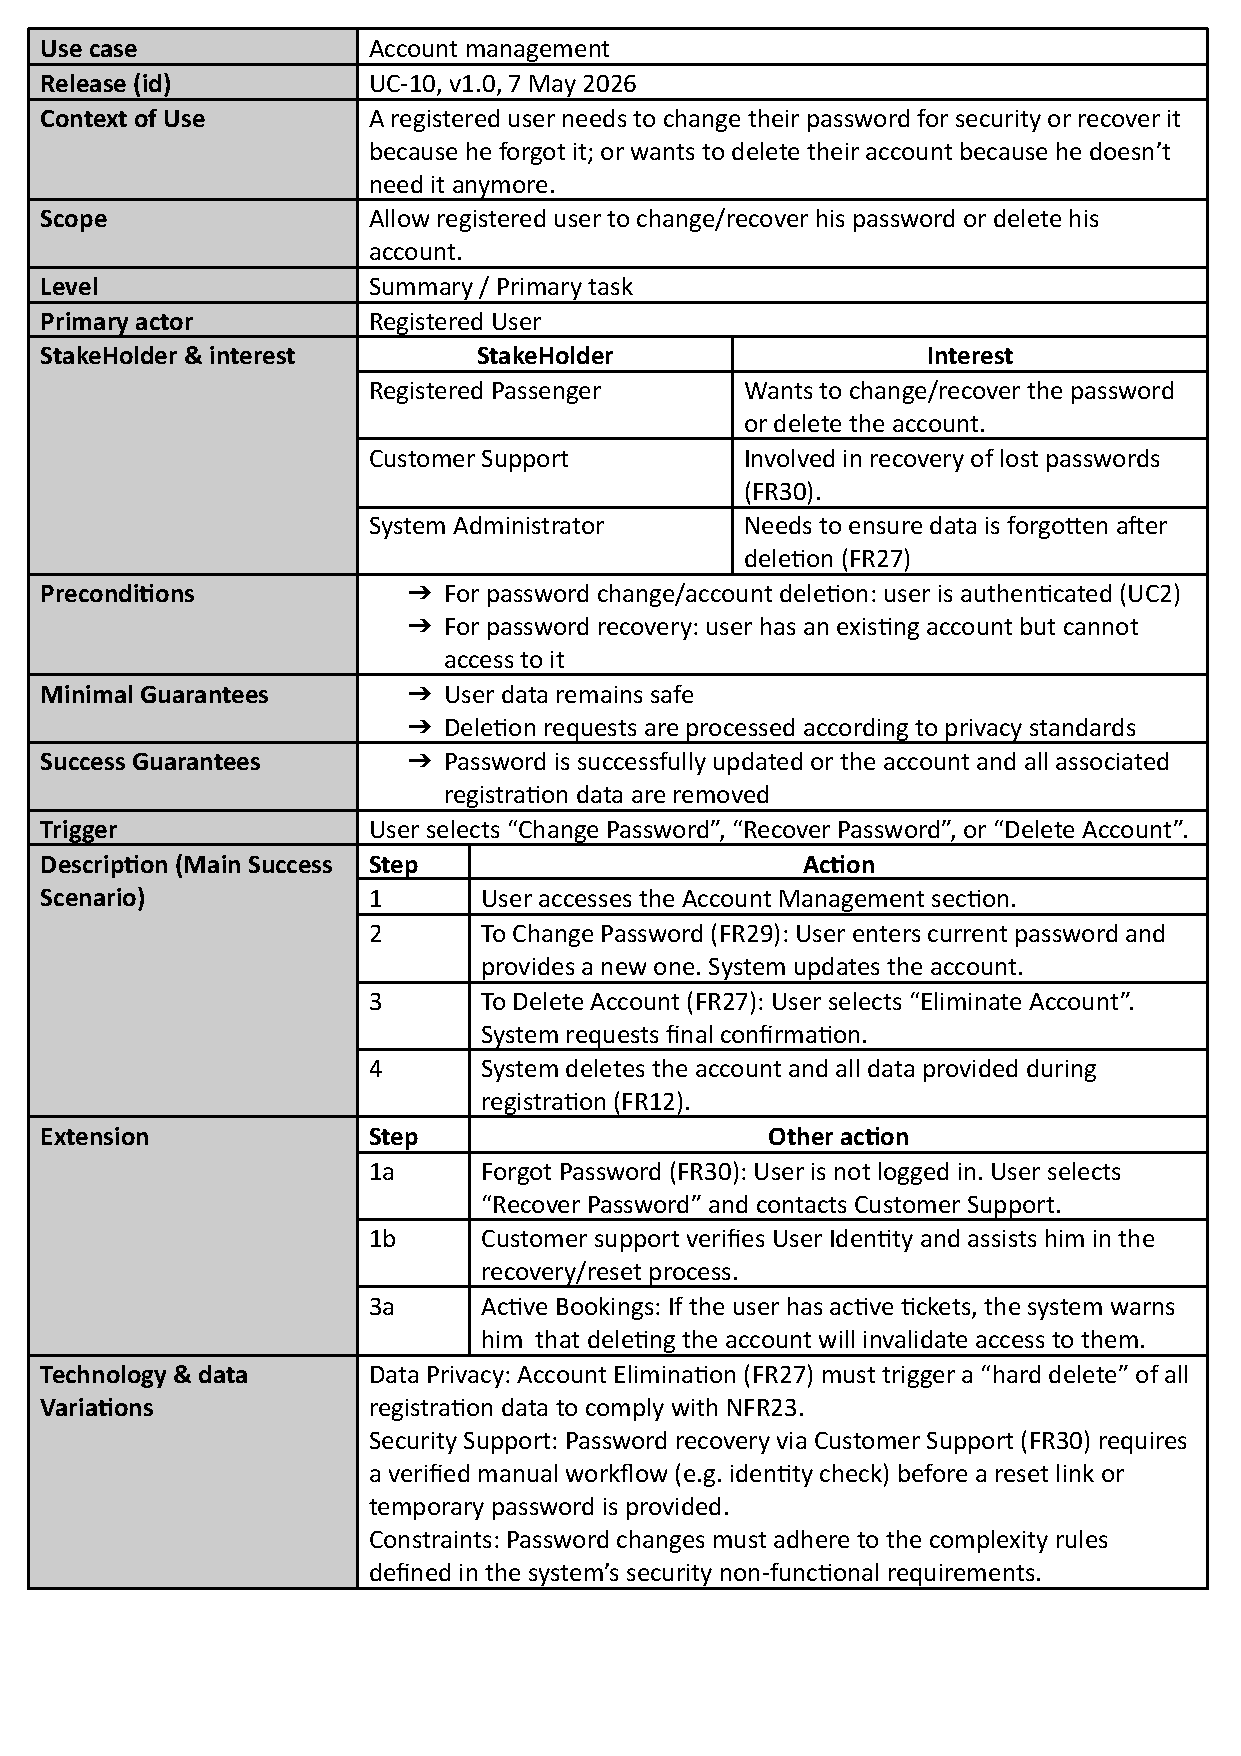
\includegraphics[width=0.9\textwidth]{UC10table.pdf}
\end{figure}
\begin{landscape}
\begin{figure}[H]
    \centering
    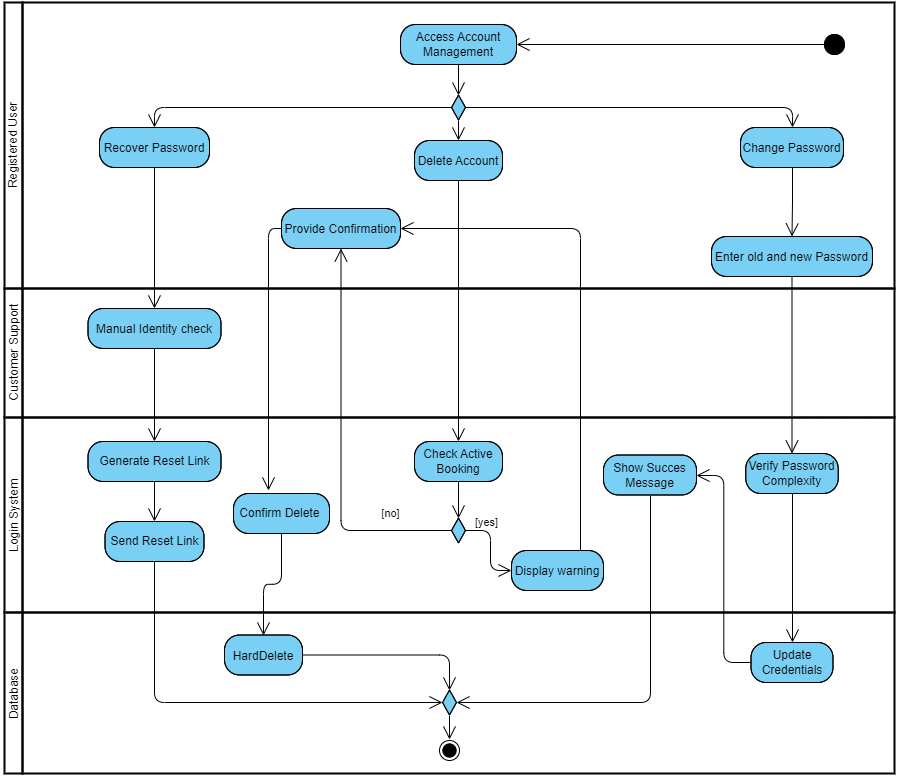
\includegraphics[width=1.1\textwidth]{UC10-activity diagram.png}
\end{figure}
\begin{figure}[H]
    \centering
    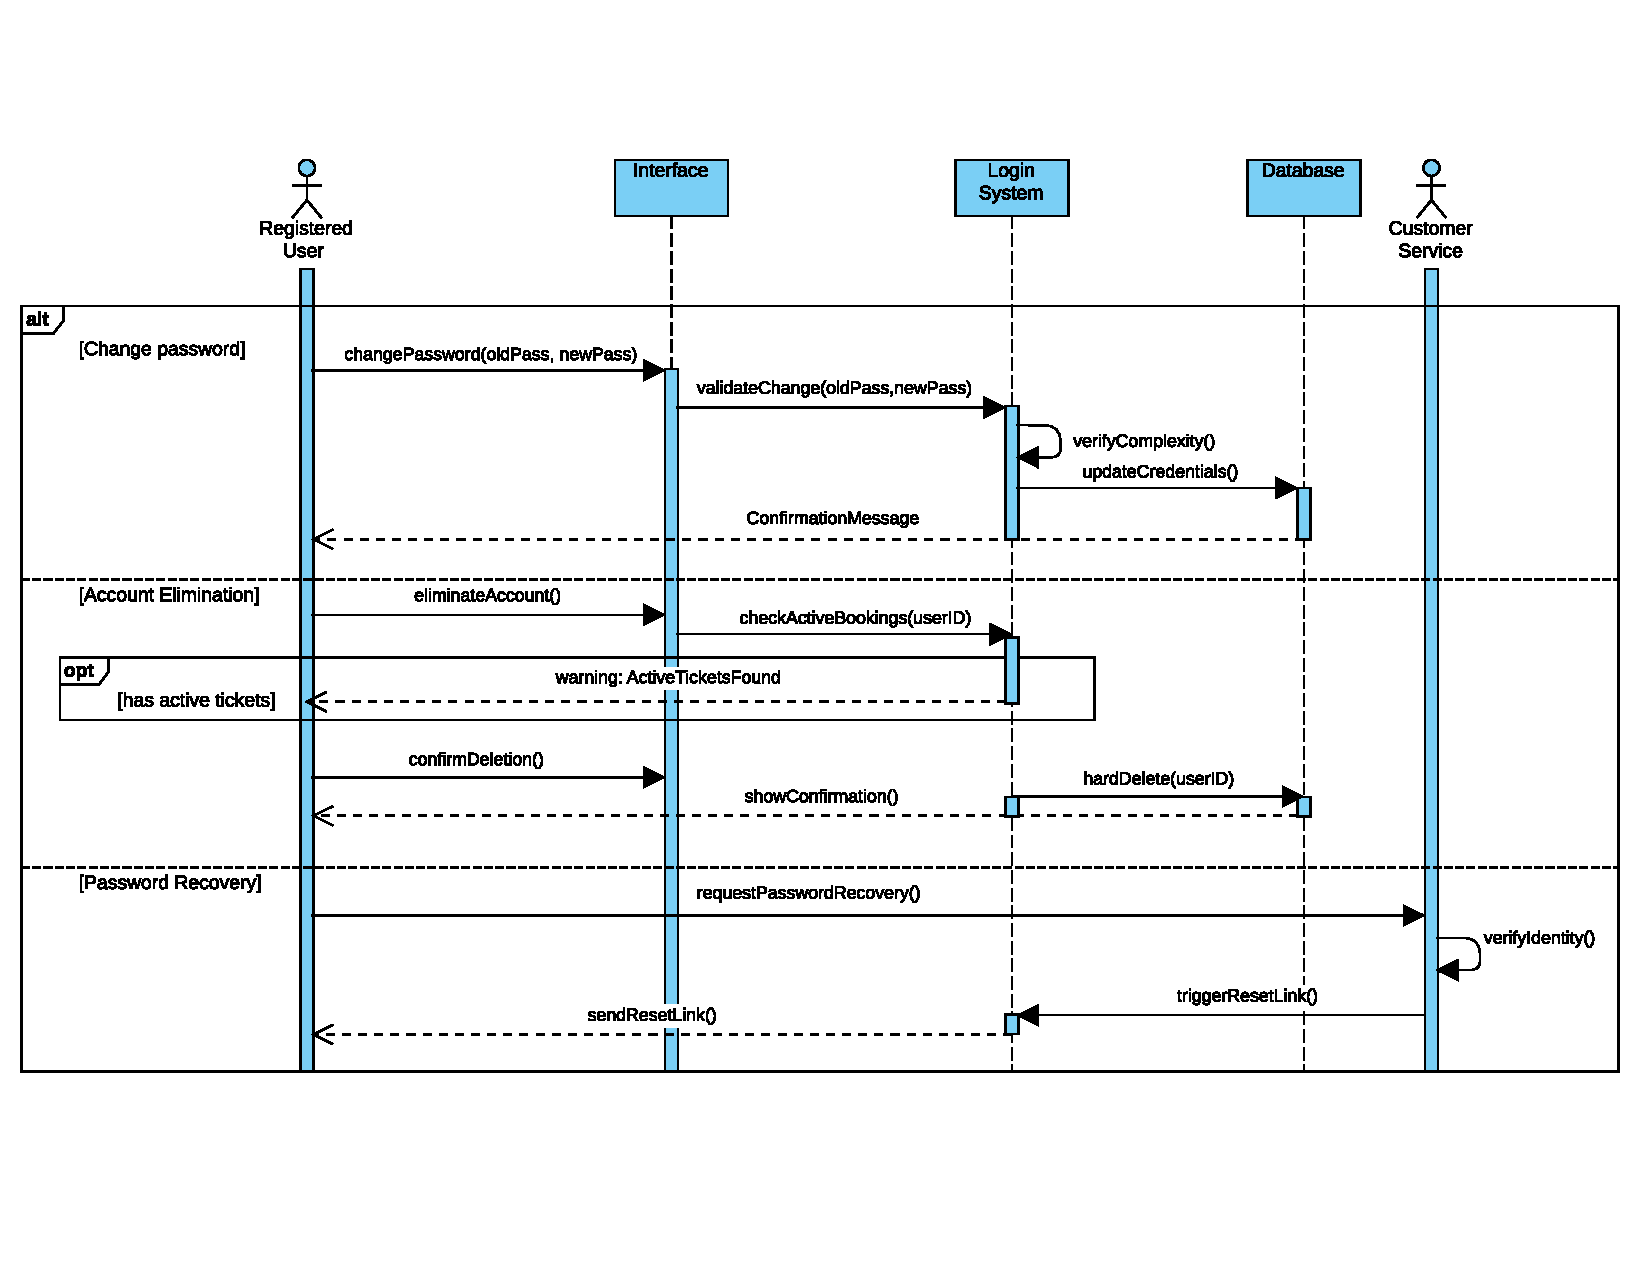
\includegraphics[width=1.3\textwidth]{UC10-sequence diagram.pdf}
\end{figure}
\end{landscape}

\subsection{UC11: Customer Support}
%\textbf{Related Functional Requirements:} FR22 
\begin{figure}[H]
    \centering
    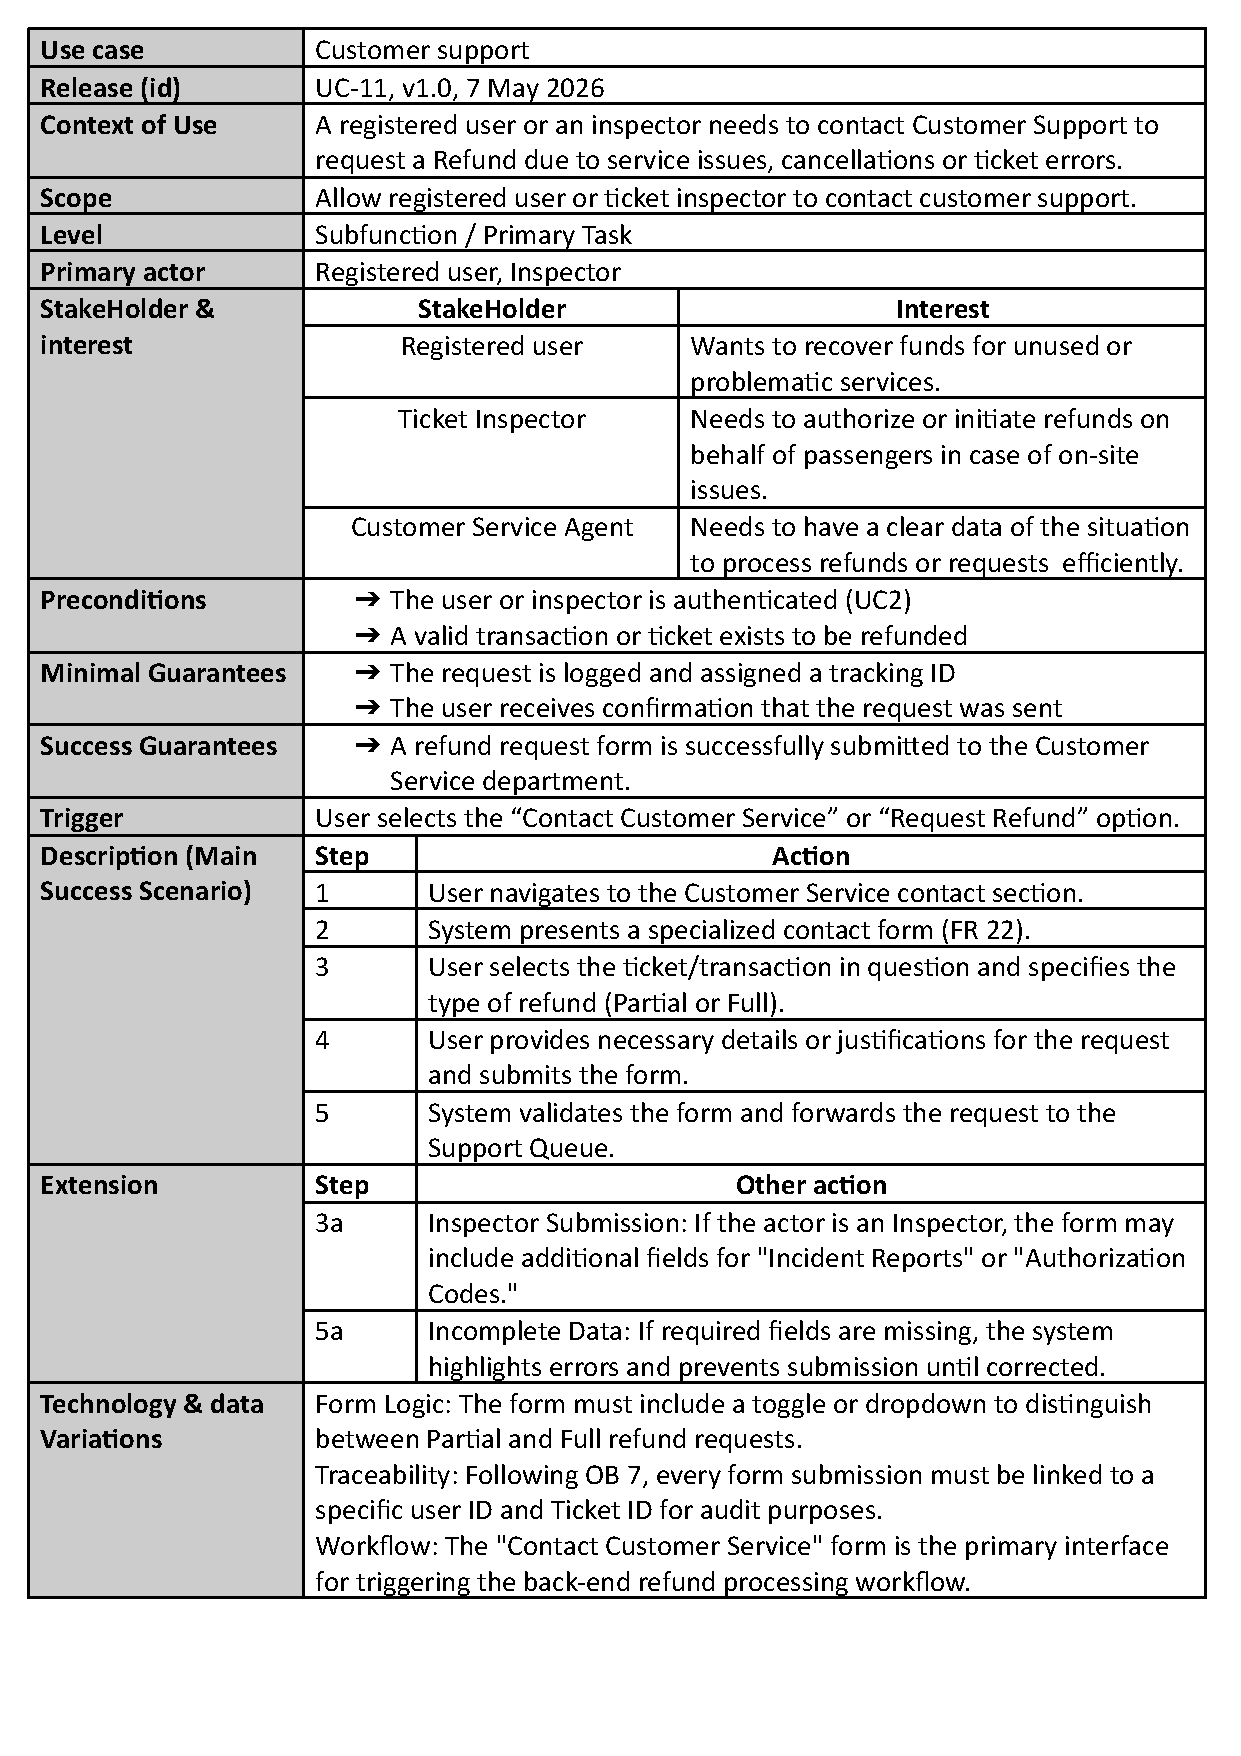
\includegraphics[width=0.9\textwidth]{UC11table.pdf}
\end{figure}
\begin{figure}[H]
    \centering
    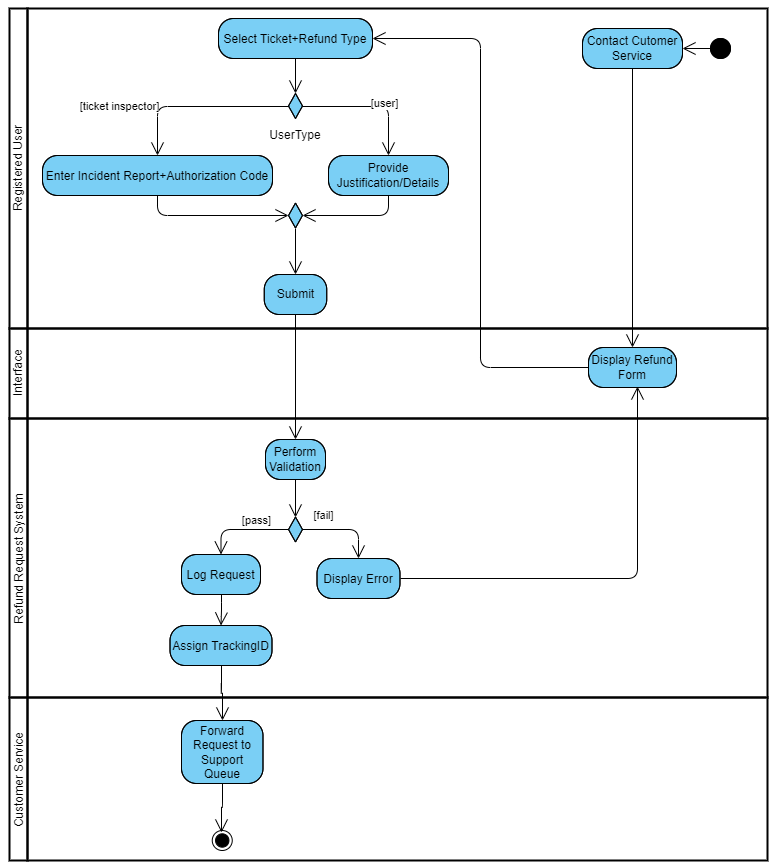
\includegraphics[width=1.0\textwidth]{UC11-activity diagram.png}
\end{figure}
\begin{landscape}
\begin{figure}[H]
    \centering
    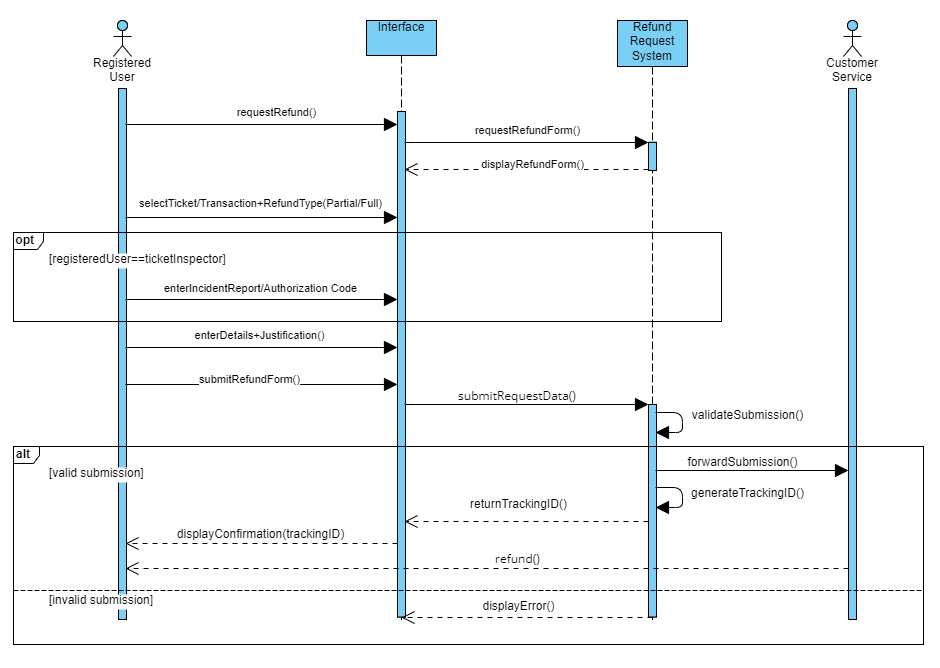
\includegraphics[width=1.2\textwidth]{UC11-sequence diagram.png}
\end{figure}
\end{landscape}

\subsection{UC12: Inspector Operations Management}
%\textbf{Related Functional Requirements:} FR24, FR26 
\begin{figure}[H]
    \centering
    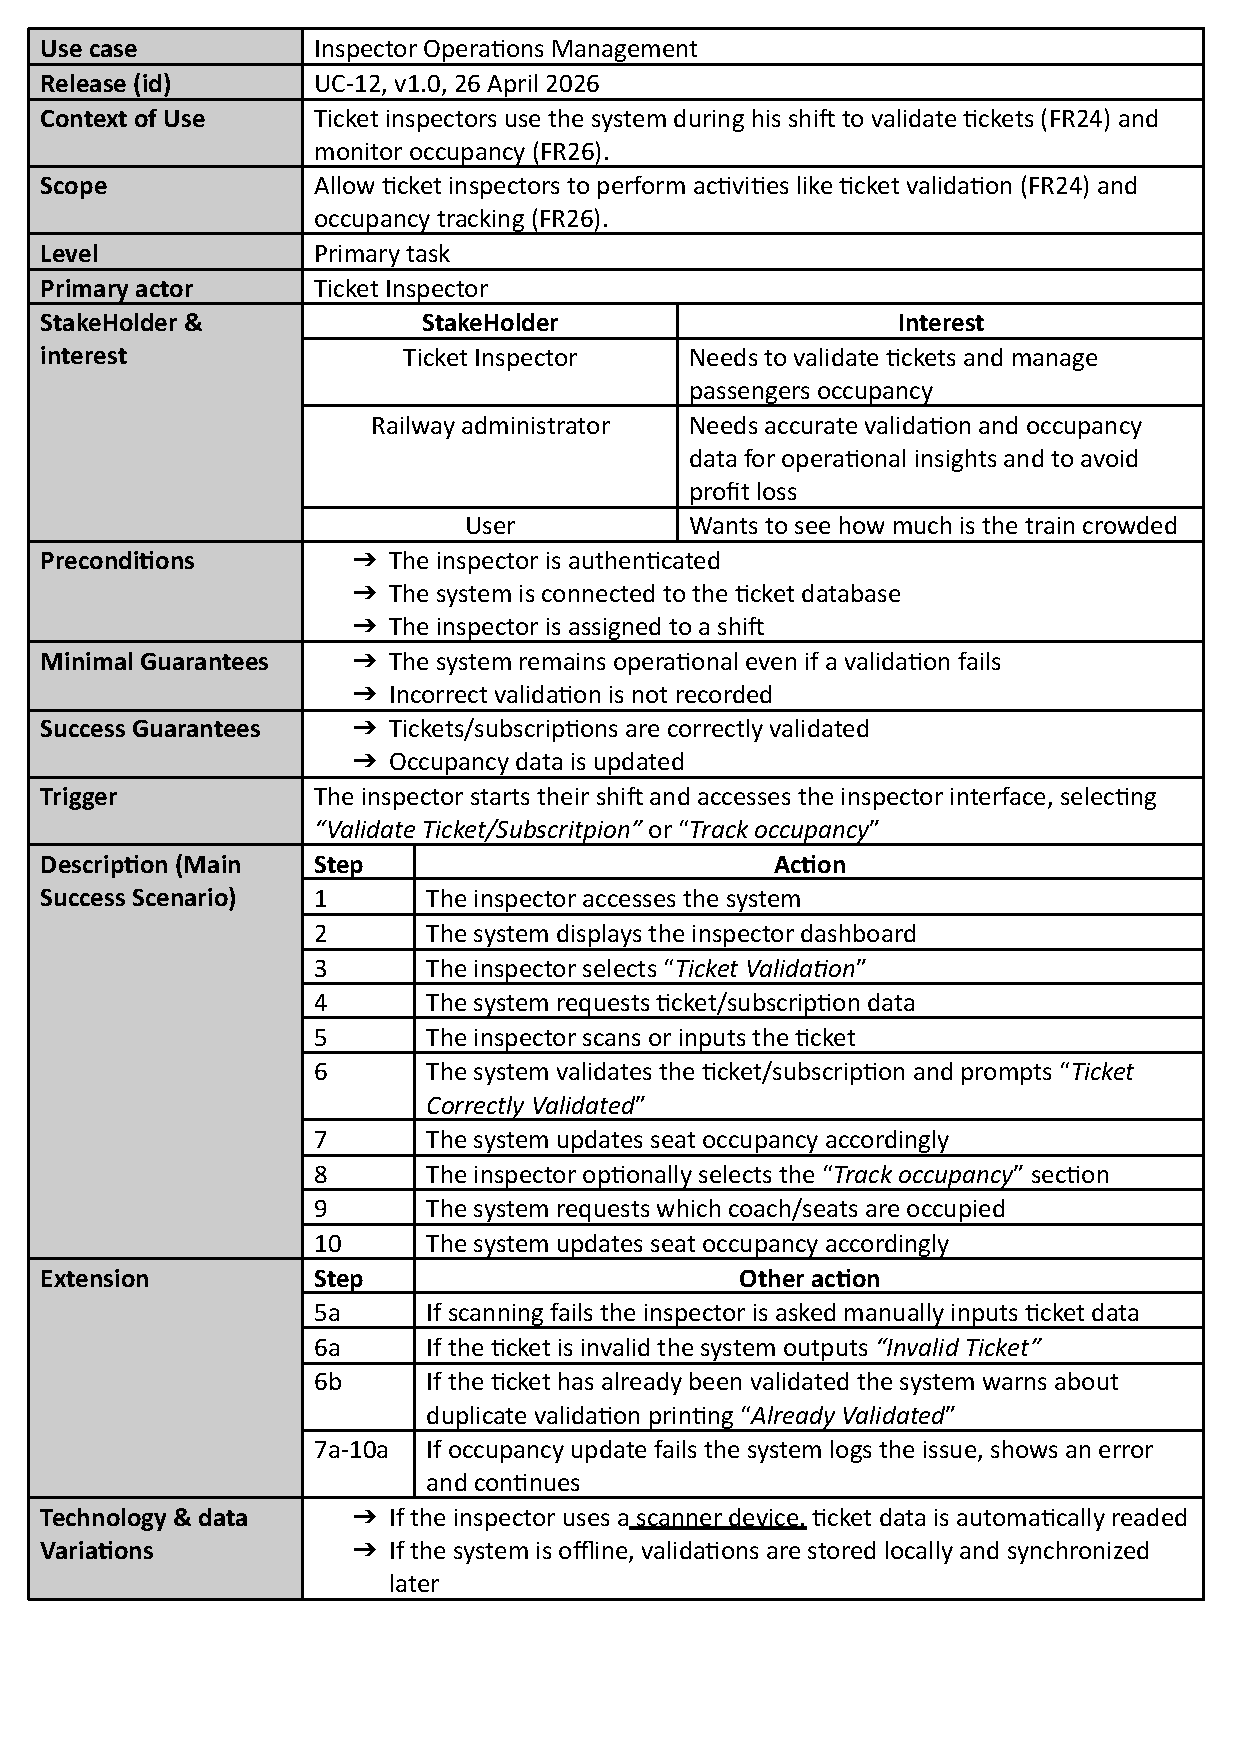
\includegraphics[width=0.9\textwidth]{UC12table.pdf}
\end{figure}
\begin{landscape}
\begin{figure}[H]
    \centering
    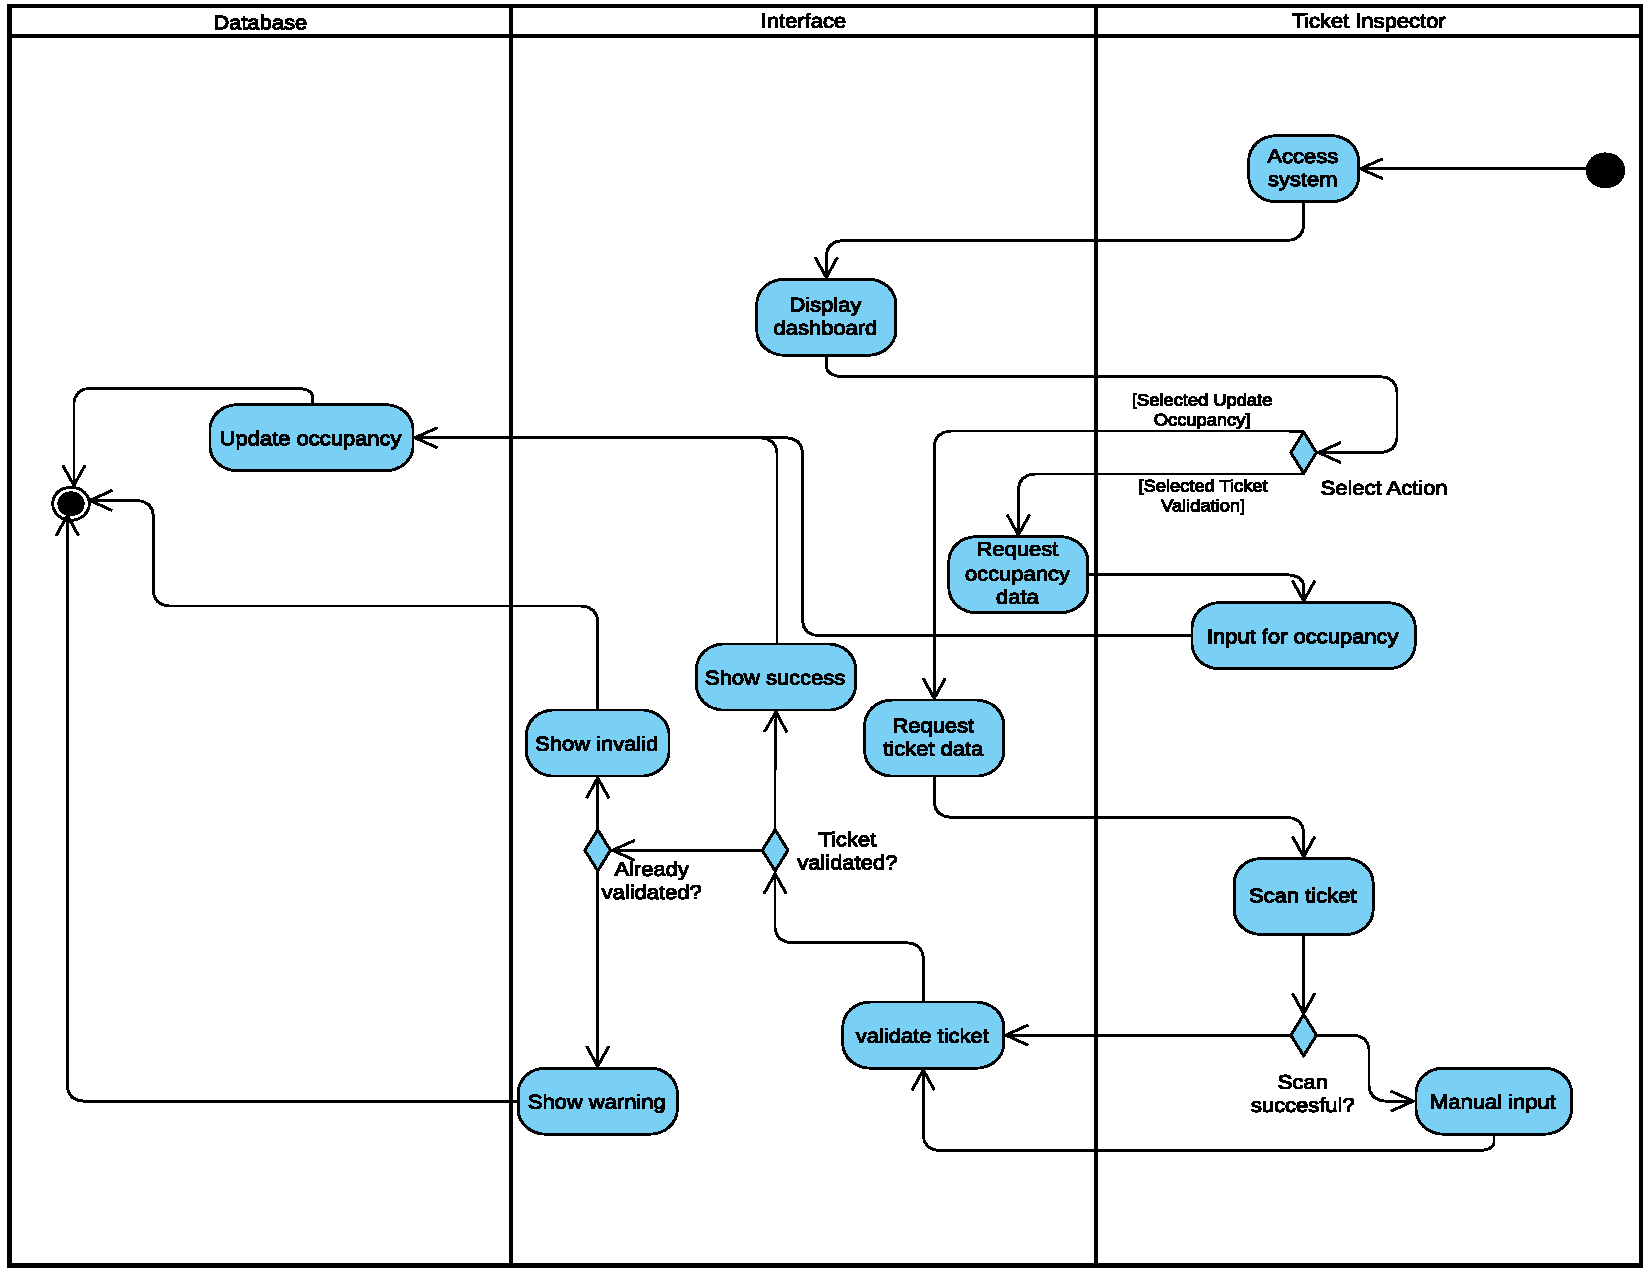
\includegraphics[width=1.25\textwidth]{UC12-activity diagram.pdf}
\end{figure}
\end{landscape}
\begin{figure}[H]
    \centering
    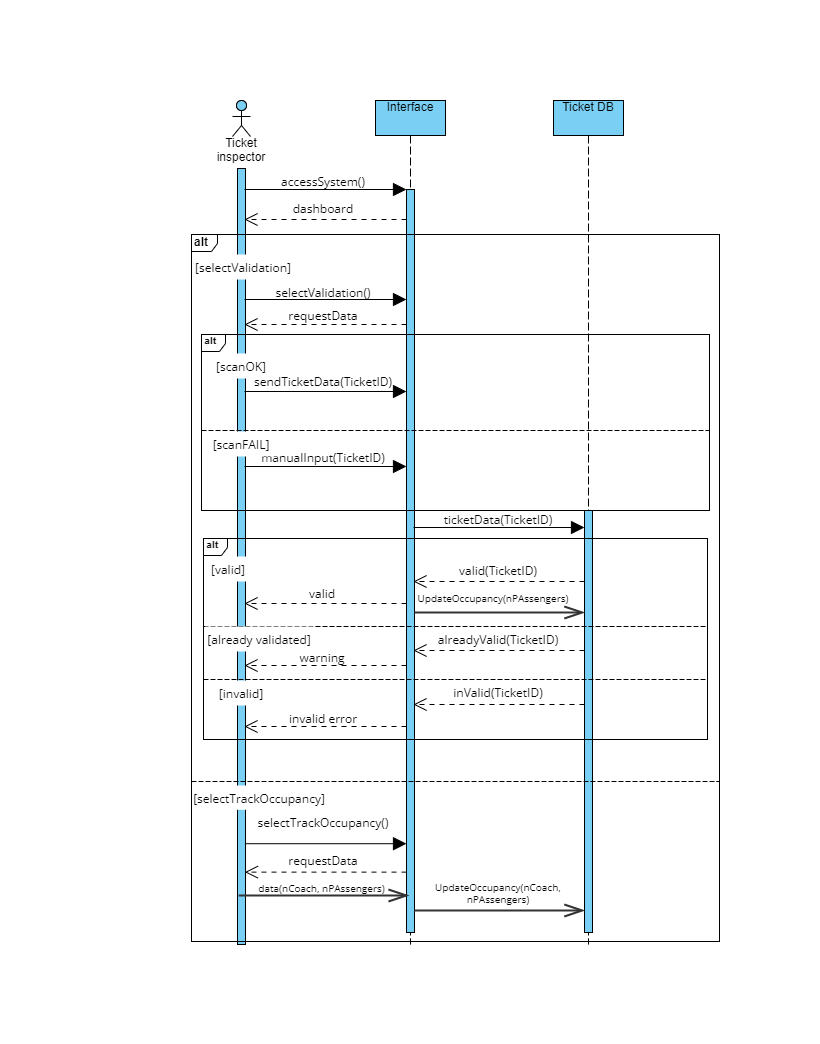
\includegraphics[width=1.0\textwidth]{UC12-sequence diagram.png}
\end{figure}

\subsection{UC13: Shift Schedule Visualization}
%\textbf{Related Functional Requirements:} FR25
\begin{figure}[H]
    \centering
    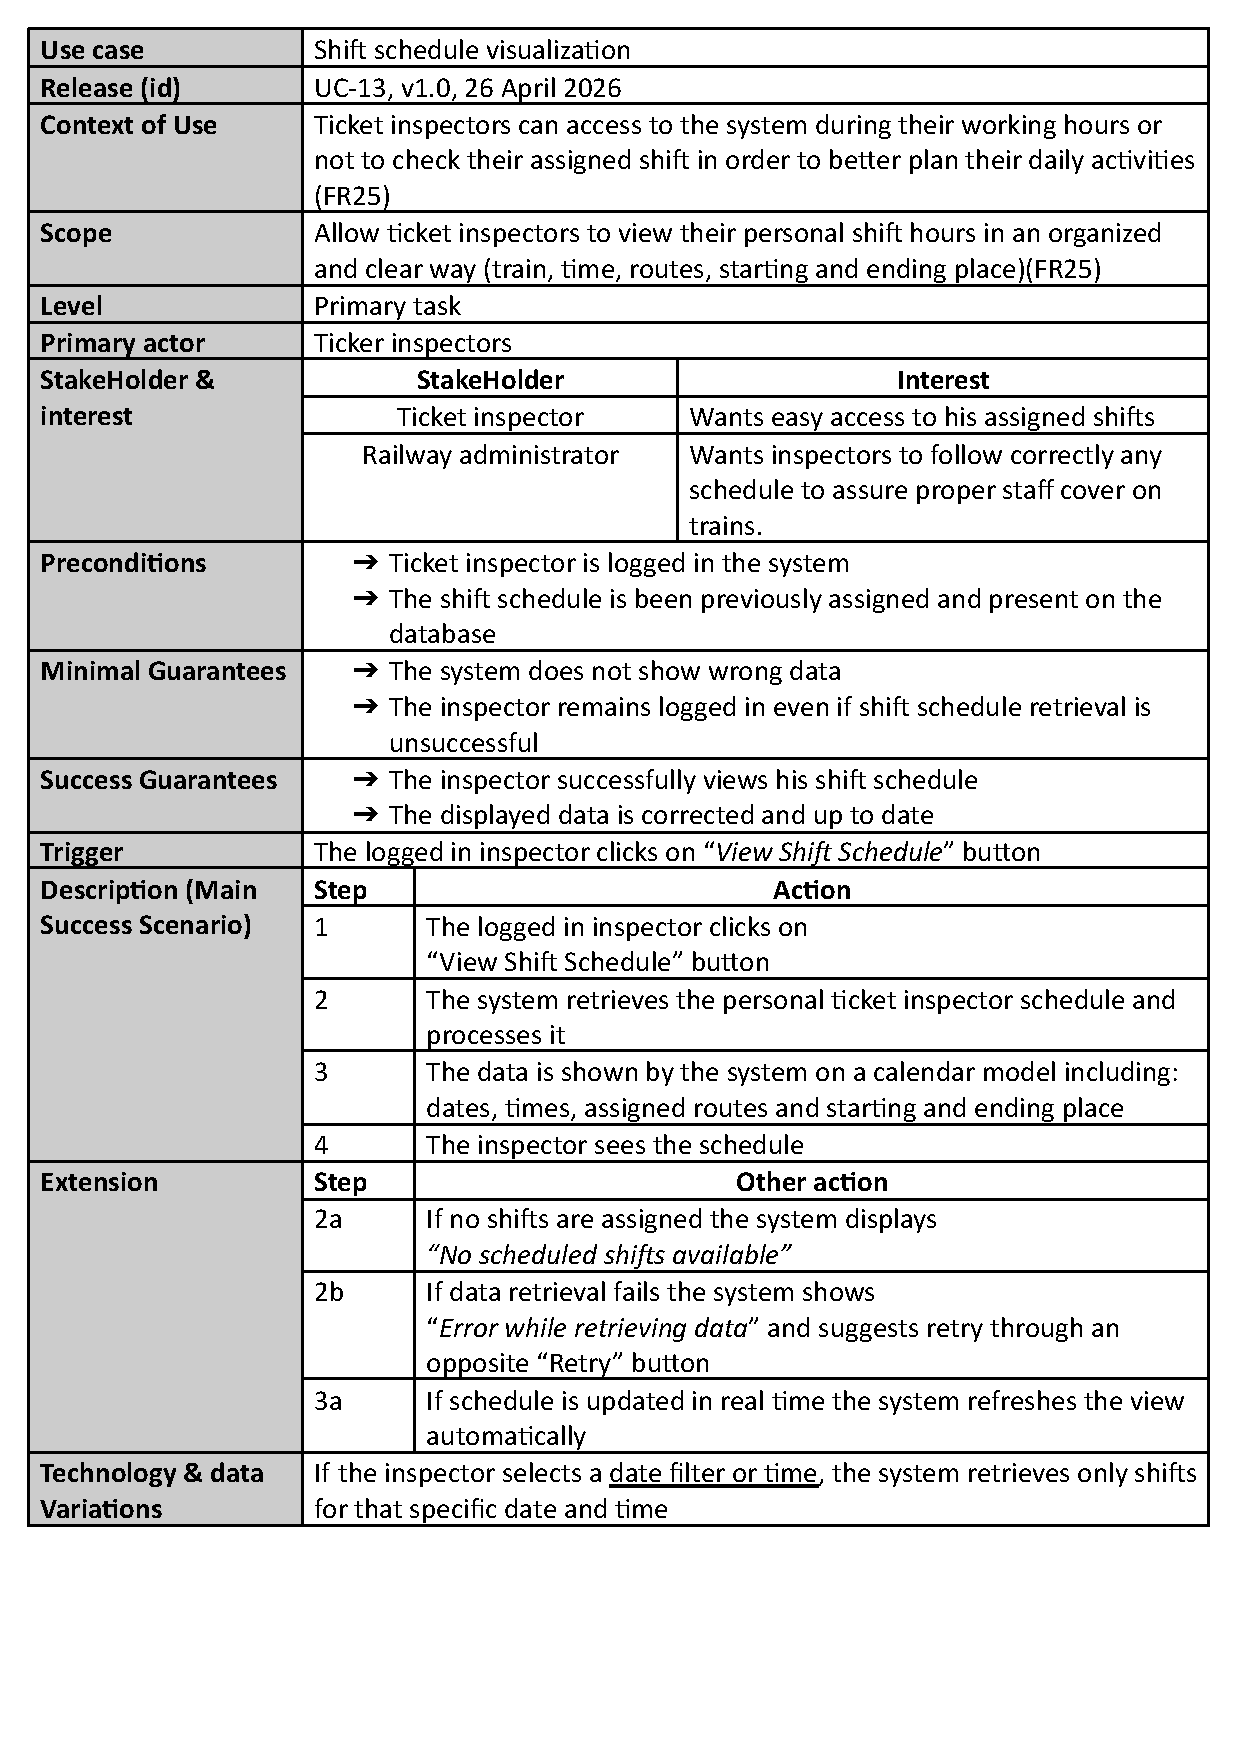
\includegraphics[width=0.9\textwidth]{UC13table.pdf}
\end{figure}
\begin{landscape}
\begin{figure}[H]
    \centering
    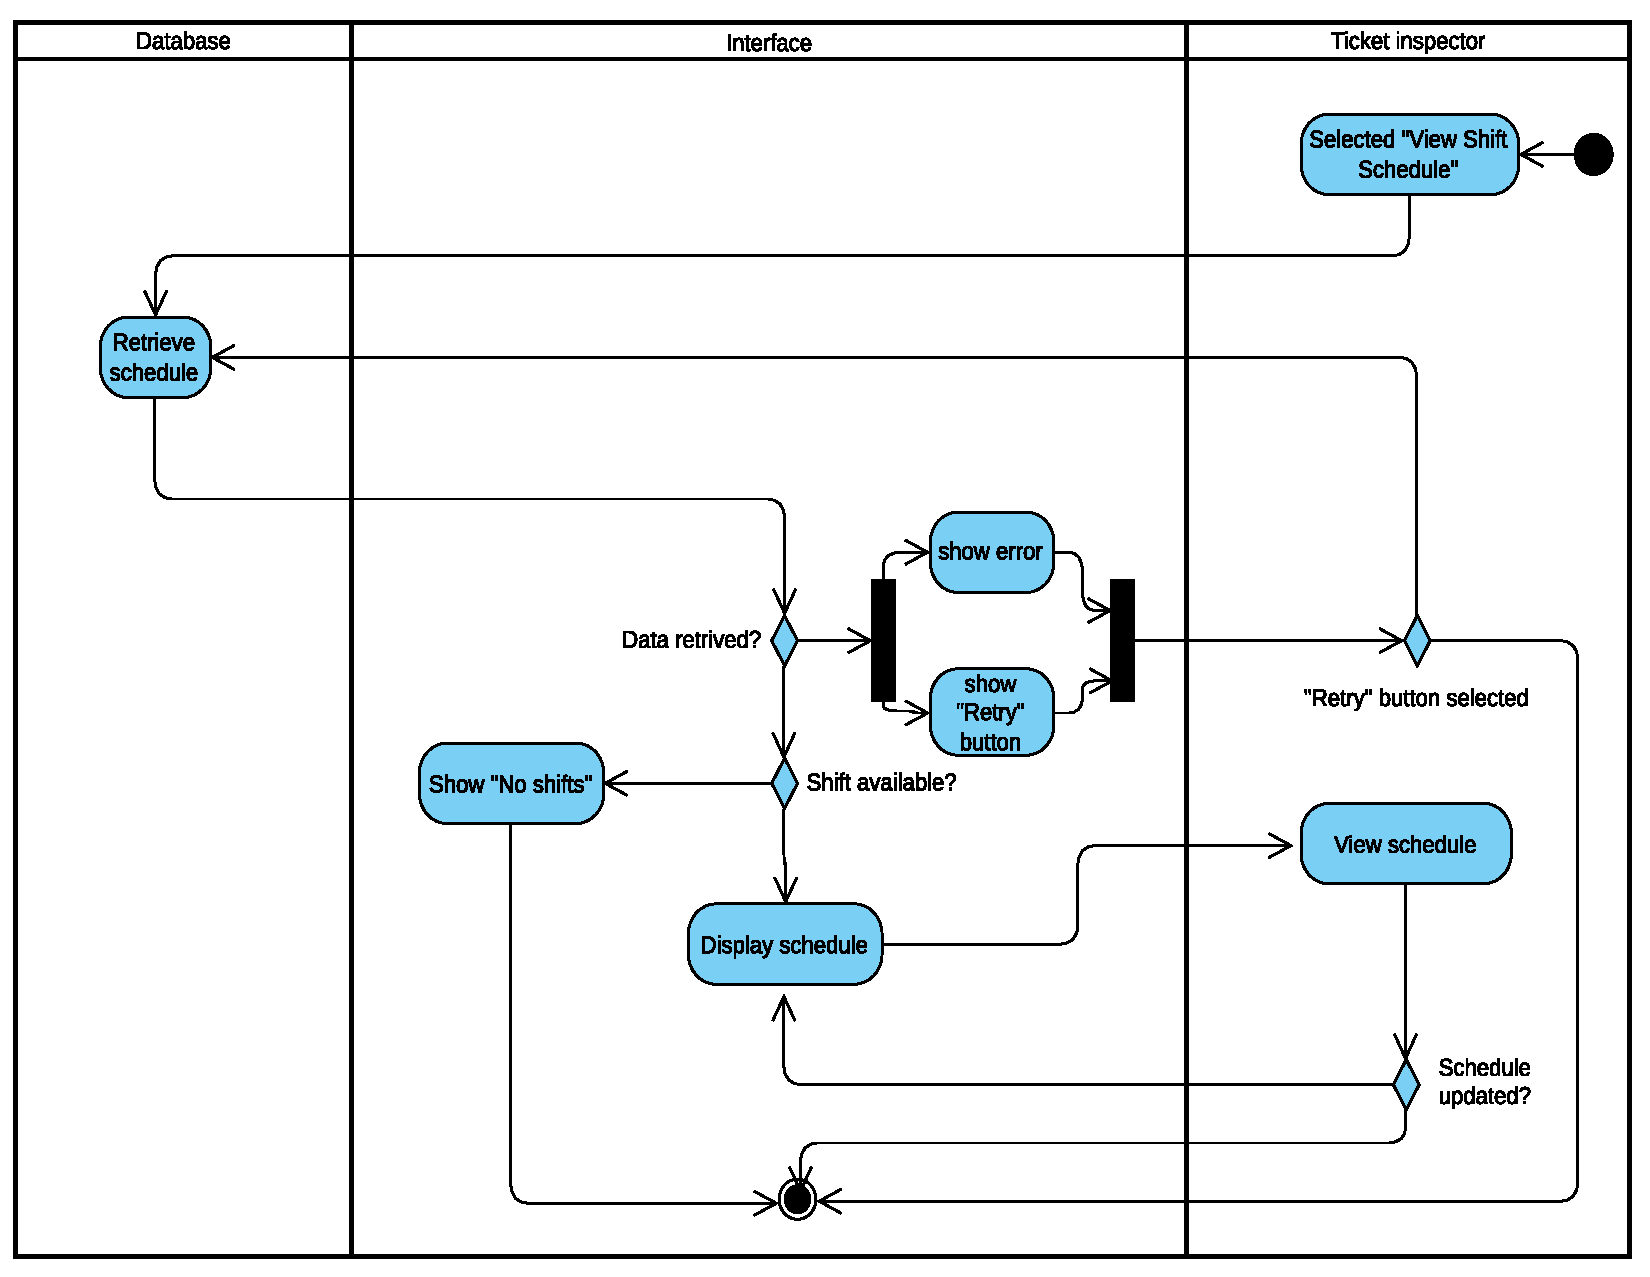
\includegraphics[width=1.25\textwidth]{UC13-activity diagram.pdf}
\end{figure}
\end{landscape}
\begin{figure}[H]
    \centering
    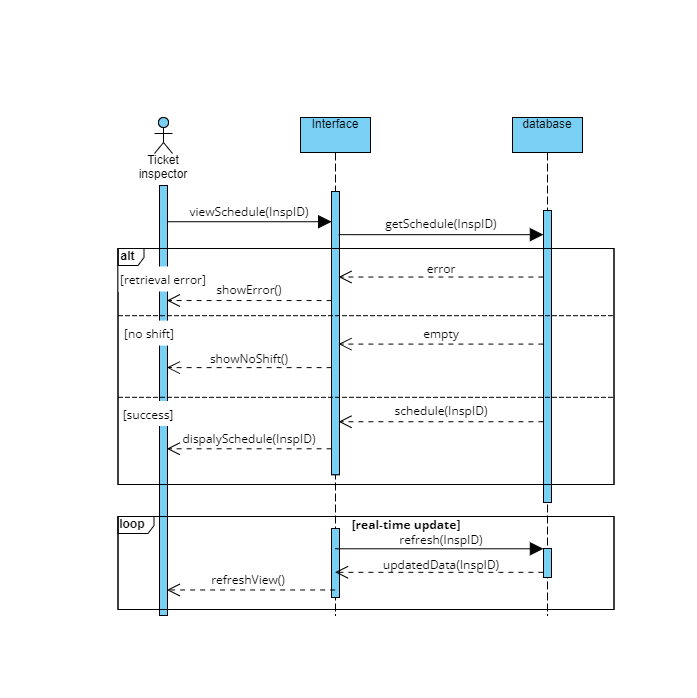
\includegraphics[width=1.1\textwidth]{UC13-sequence diagram.png}
\end{figure}
\subsection{UC14: Statistics Visualization}
%\textbf{Related Functional Requirements:} FR32 
\begin{figure}[H]   
    \centering
    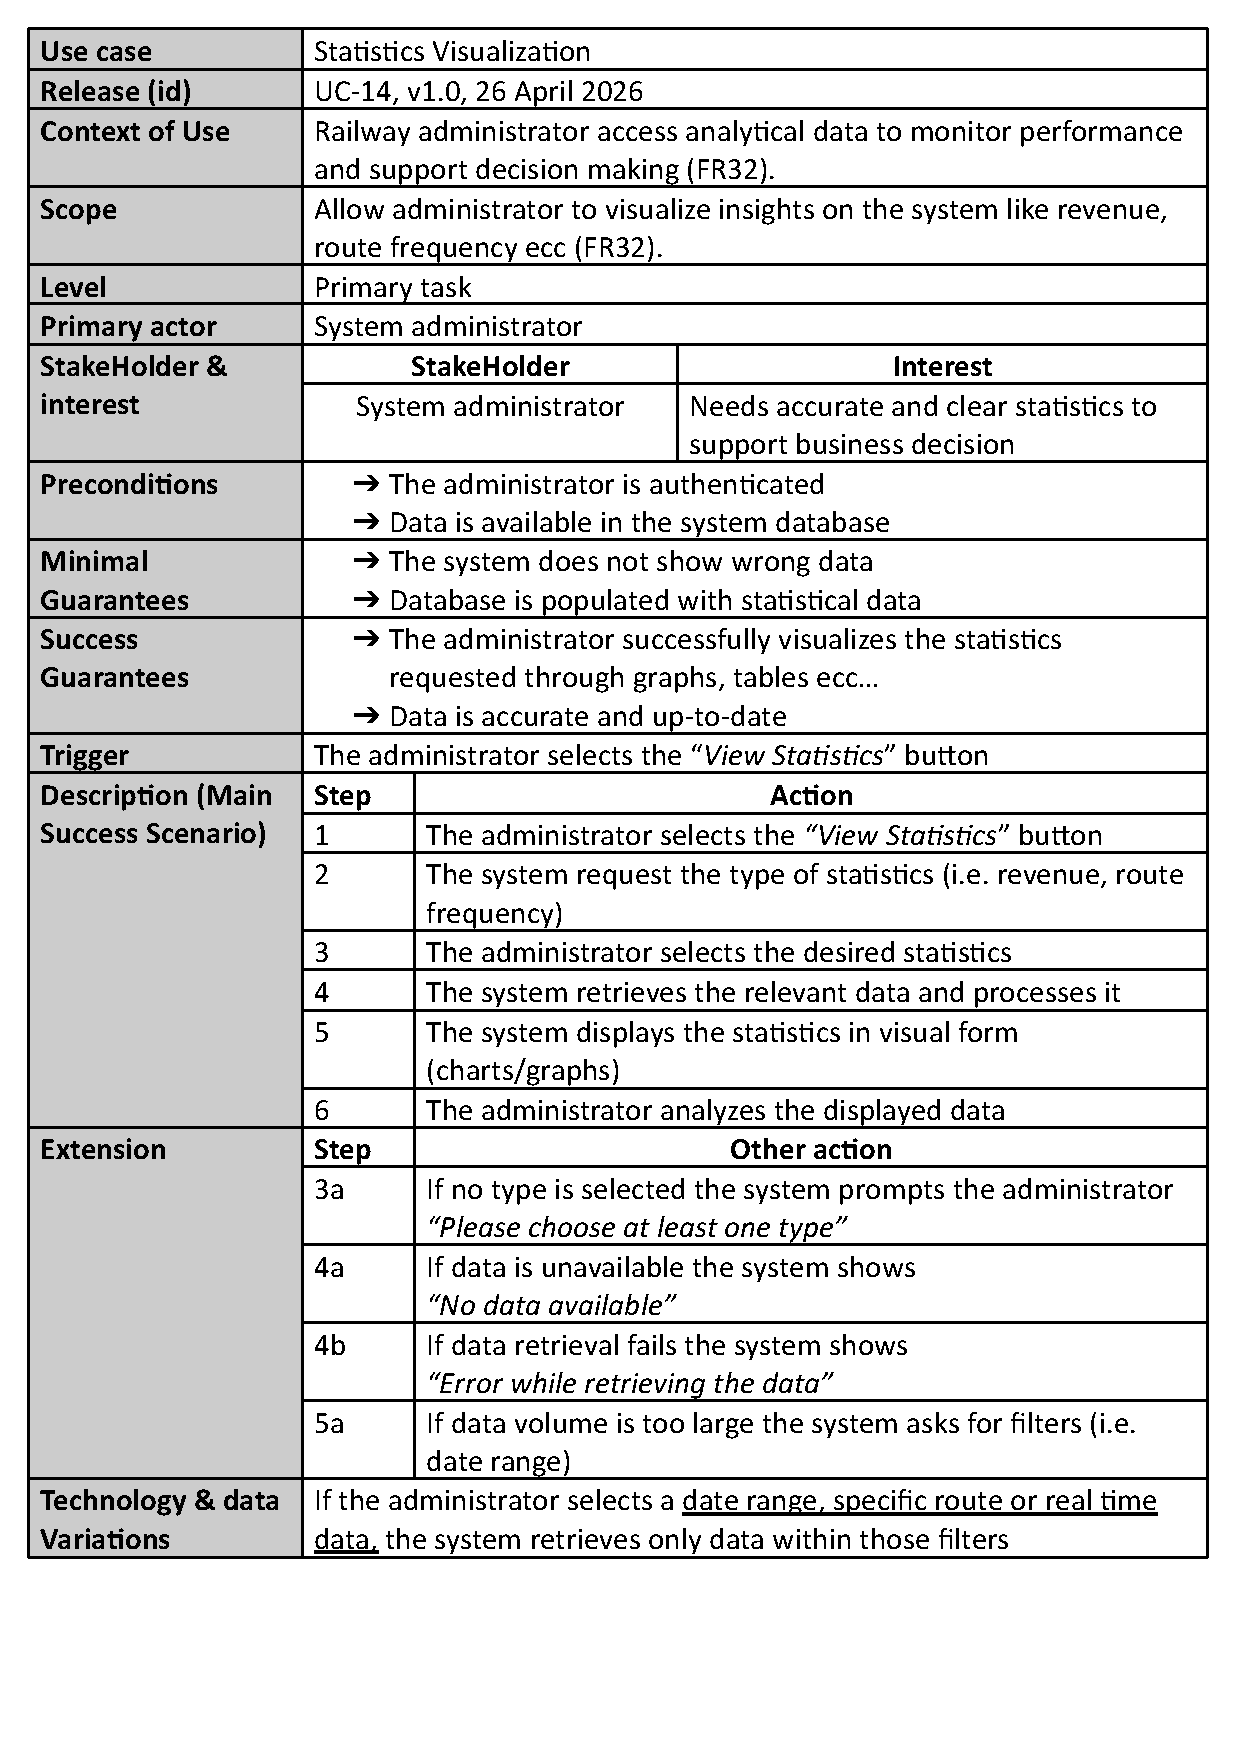
\includegraphics[width=0.9\textwidth]{UC14table.pdf}
\end{figure}
\begin{landscape}
\begin{figure}[H]
    \centering
    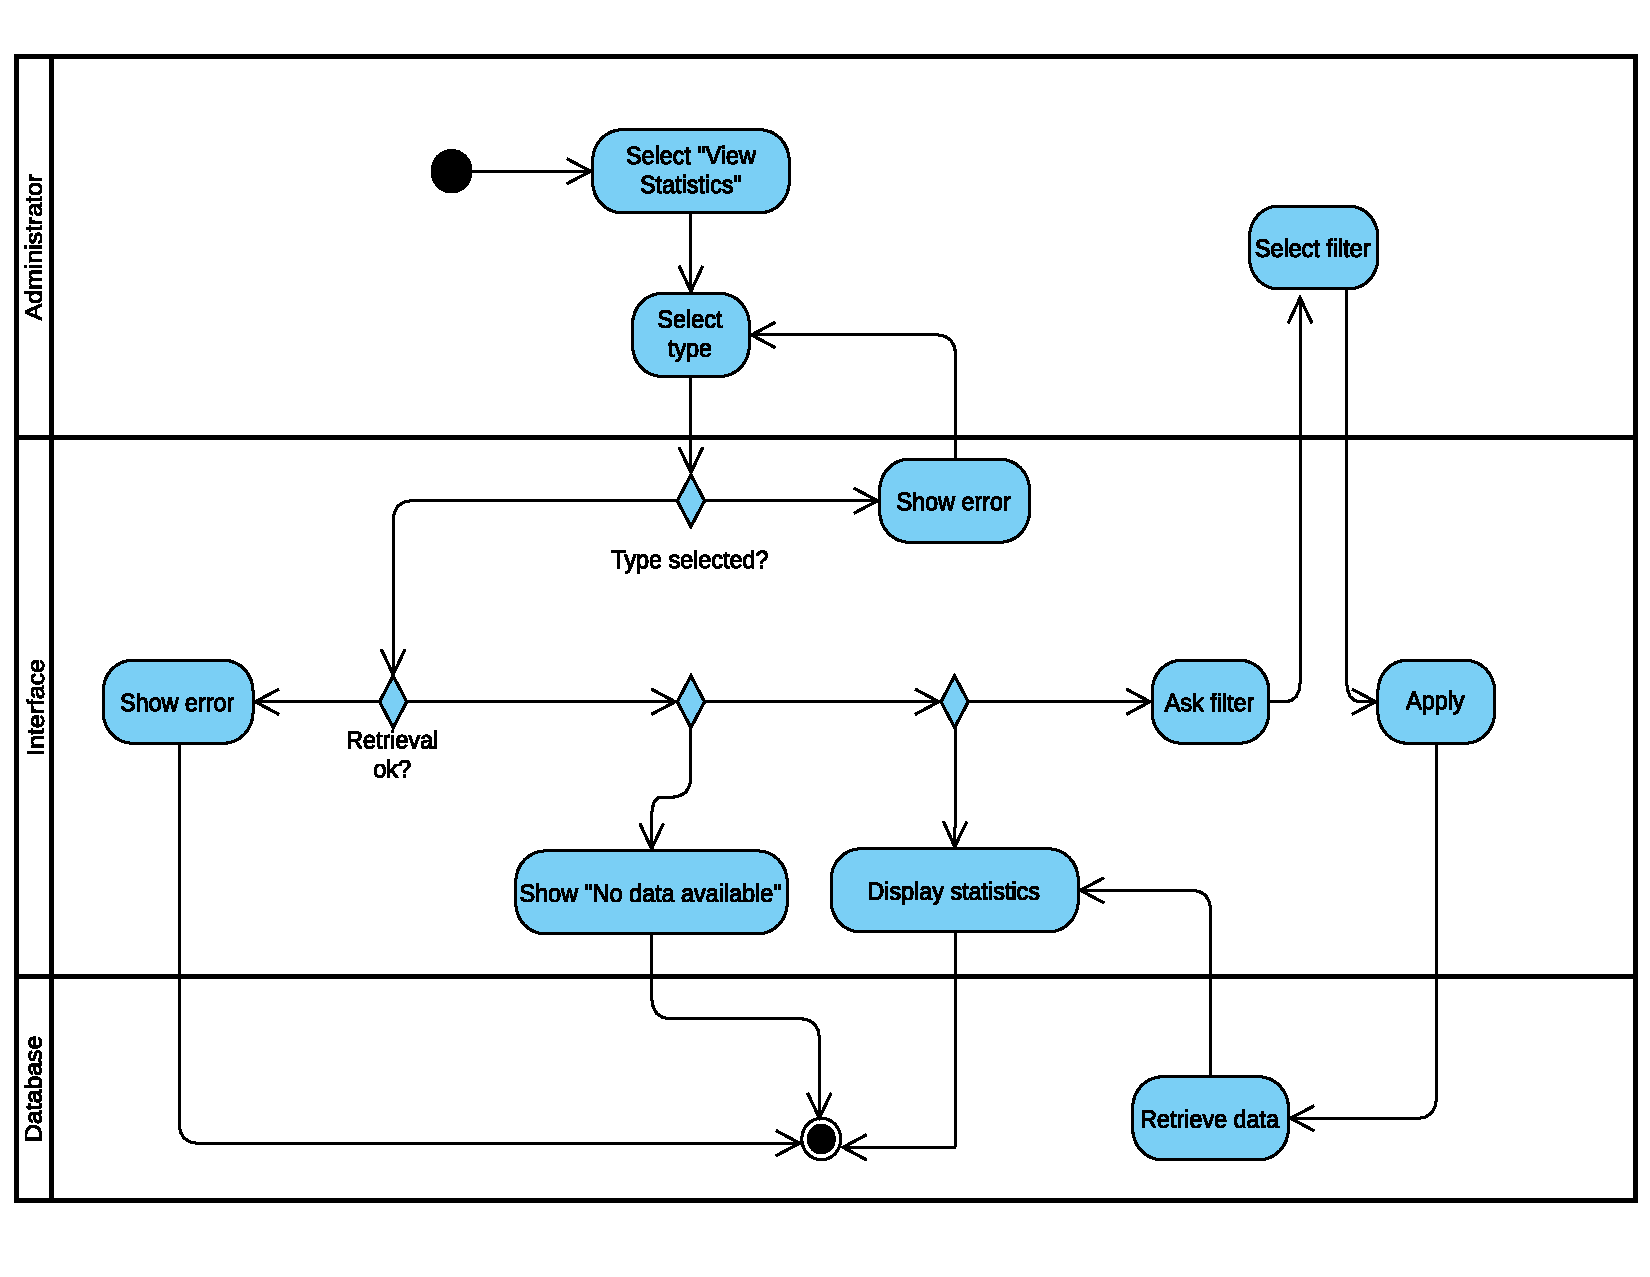
\includegraphics[width=1.25\textwidth]{UC14-activity diagram.pdf}
\end{figure}
\end{landscape}
\begin{figure}[H]
    \centering
    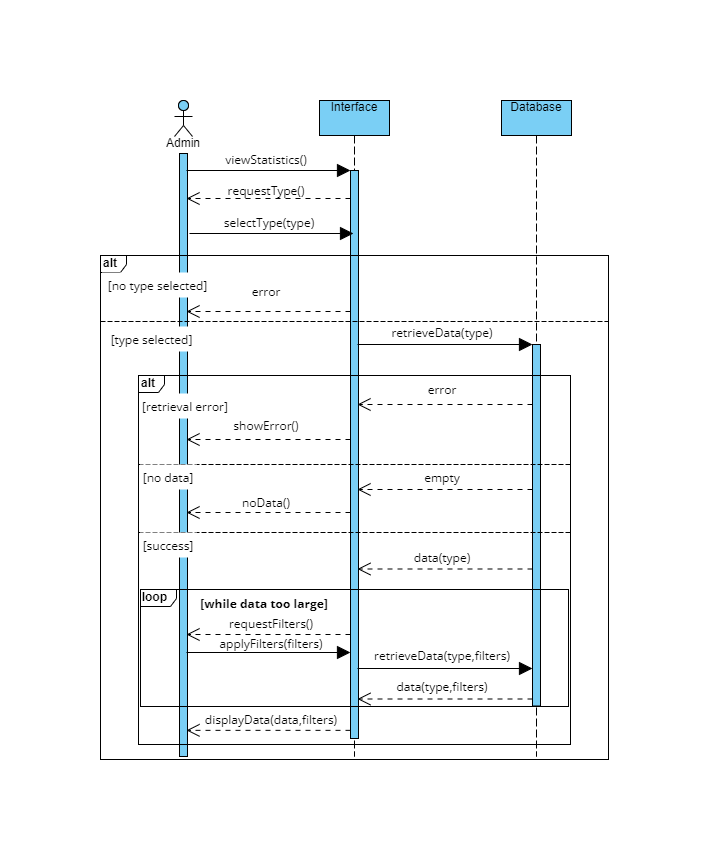
\includegraphics[width=1.0\textwidth]{UC14-sequence diagram.png}
\end{figure}
\subsection{UC15: Change Language}
%\textbf{Related Functional Requirements:} FR7 
\begin{figure}[H]
    \centering
    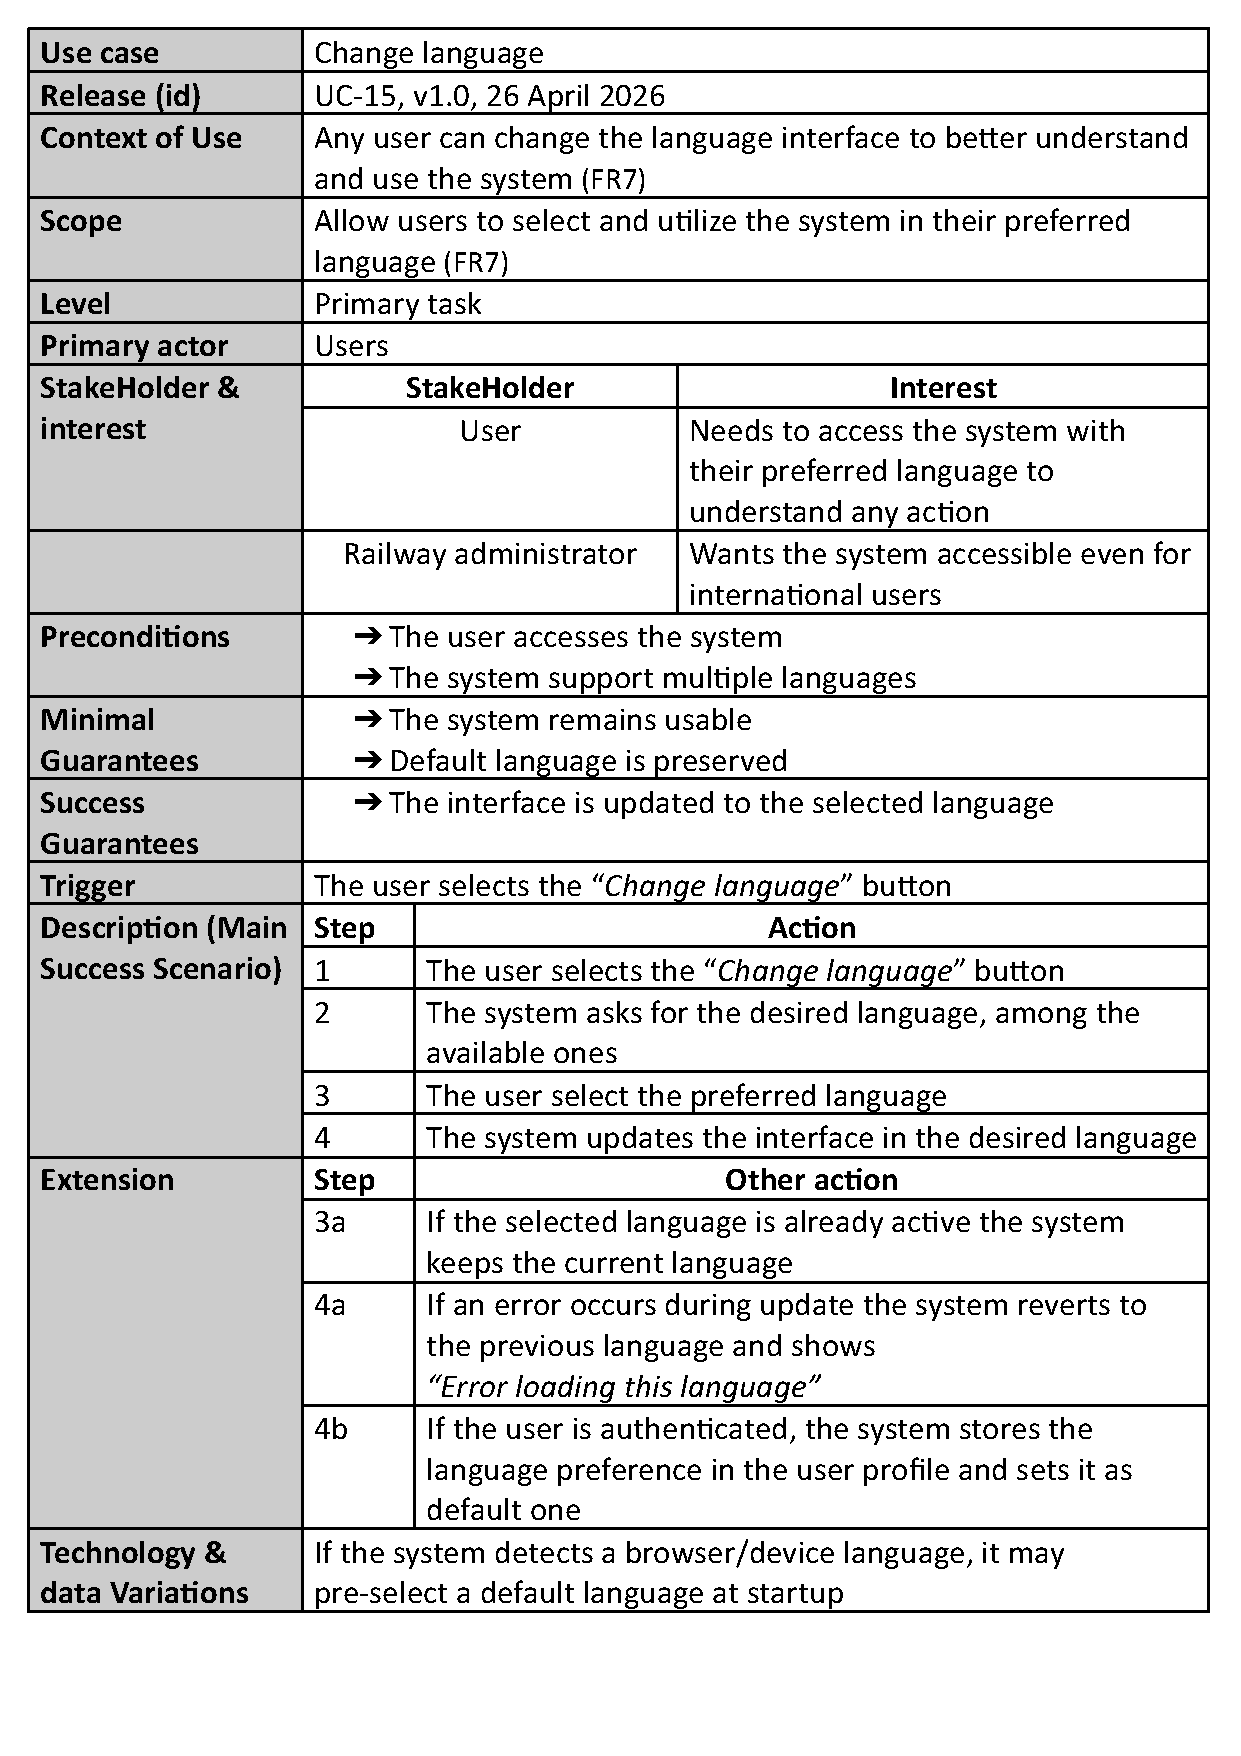
\includegraphics[width=0.9\textwidth]{UC15table.pdf}
\end{figure}
\begin{landscape}
\begin{figure}[H]
    \centering
    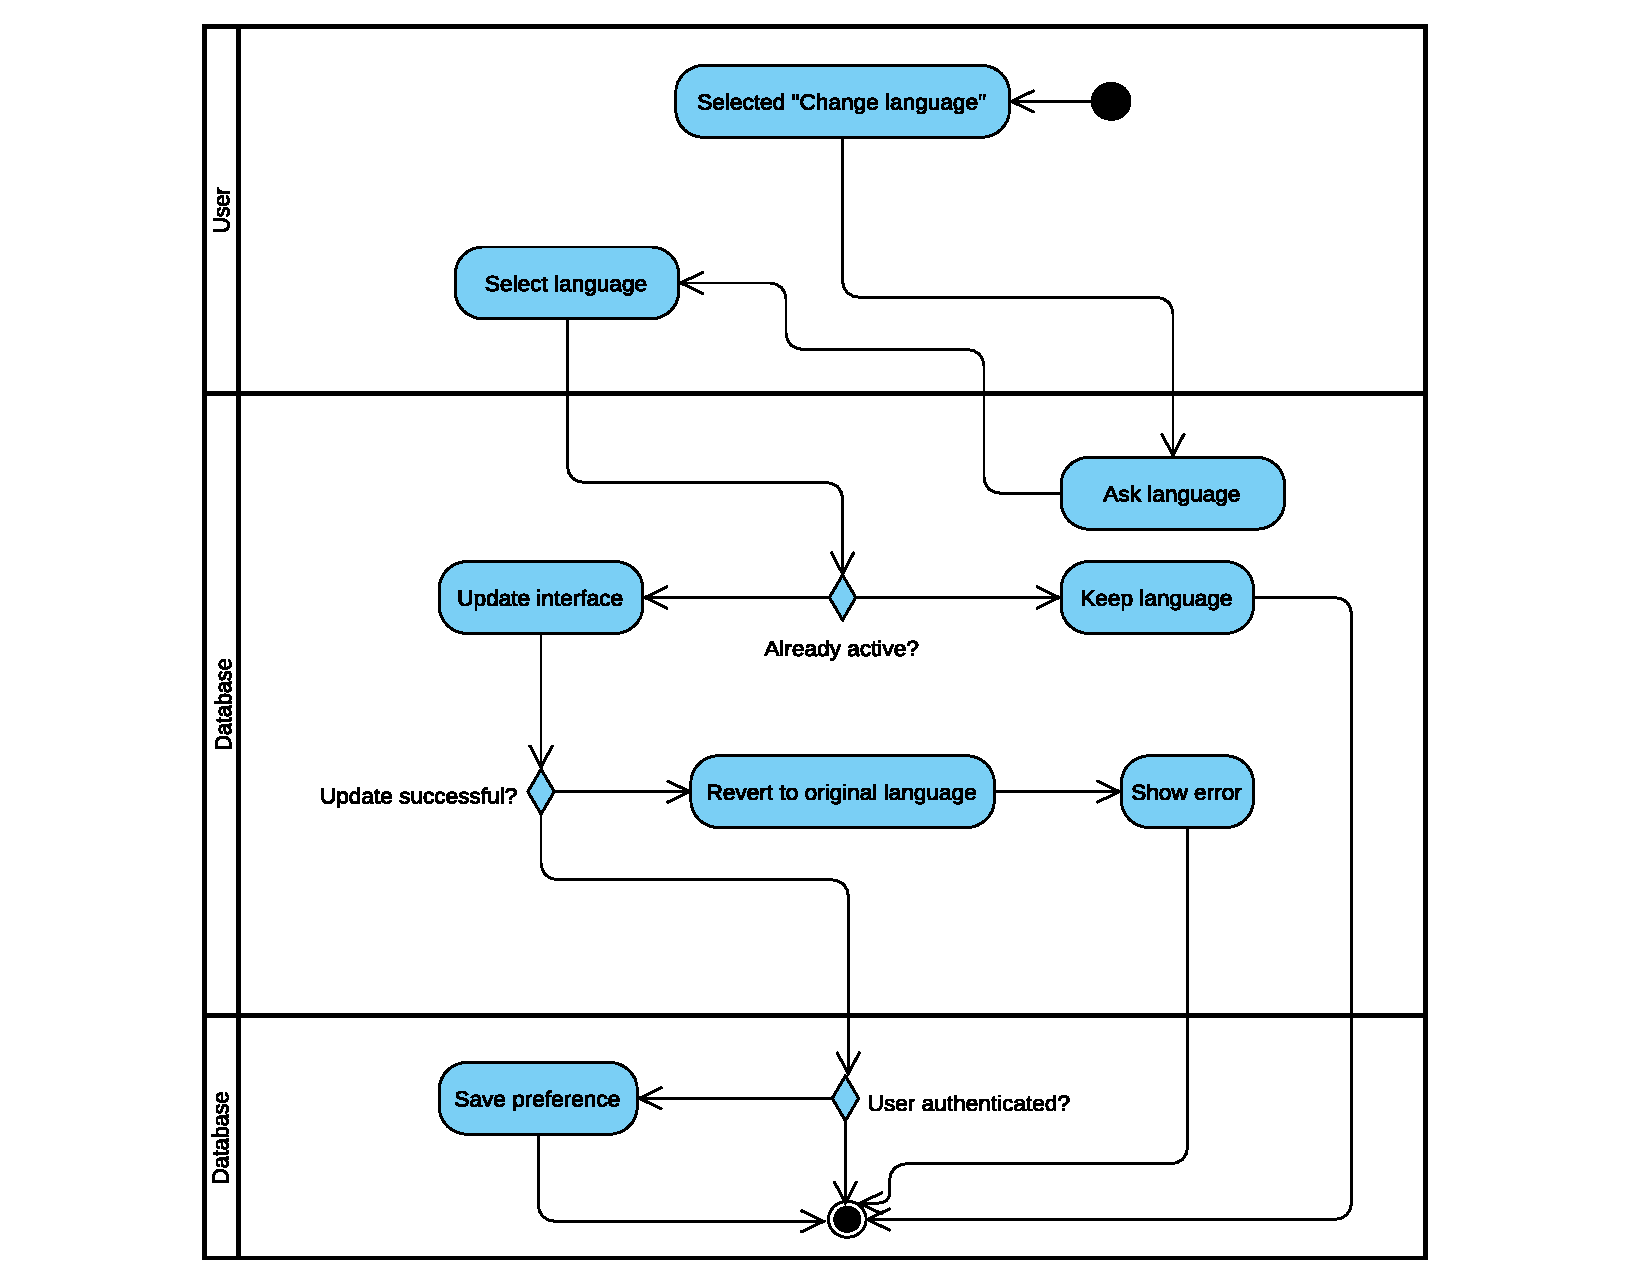
\includegraphics[width=1.25\textwidth]{UC15-activity diagram.pdf}
\end{figure}
\end{landscape}
\begin{figure}[H]
    \centering
    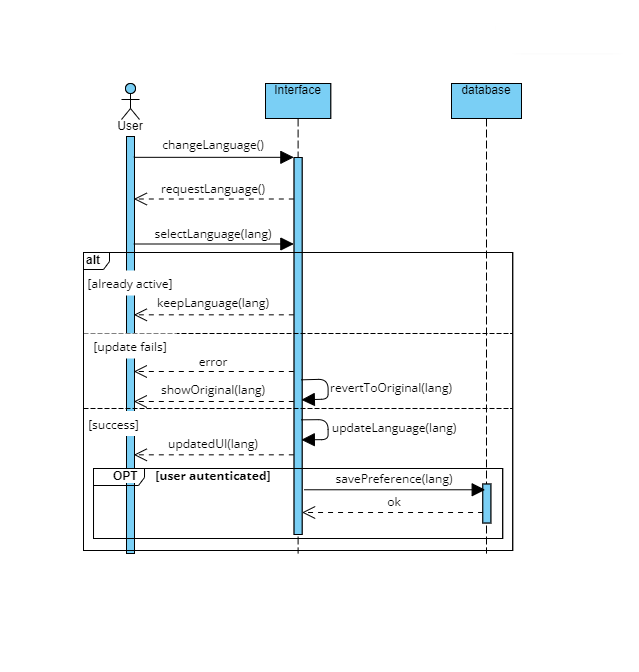
\includegraphics[width=1.1\textwidth]{UC15-sequence diagram.png}
\end{figure}
\newpage
\section{Mapping of Use Cases to FR and NFR}
\begin{table}[h]
\centering
\label{tab:uc_fr_nfr}
\scalebox{0.8}{%
\begin{tabular}{|>{\columncolor{gray!15}}c|c|c|}
\toprule
\rowcolor{gray!30} \textbf{Use Case} & \textbf{Functional Requirements} & \textbf{Non-Functional Requirements} \\
\midrule
UC1: Search Train & FR1, FR2, FR3, FR4, FR5, FR11, FR17 & NFR5, NFR6 \\ \hline
UC2: Authentication & FR12, FR28, FR34 & NFR15, NFR16, NFR18, NFR20, NFR24 \\ \hline
UC3: Admin Area Access & FR31, FR32 & NFR17 \\ \hline
UC4: Purchase & FR8, FR9, FR10, FR13, FR14, FR21 & NFR19, NFR28, NFR29\\ \hline
UC5: Check Train Status & FR15, FR33 & NFR8 \\ \hline
UC6: Boards Visualization & FR6 & --- \\ \hline
UC7: Receive Notifications & FR23 & NFR23 \\ \hline
UC8: User Dashboard / Profile & FR17, FR18, FR19, FR20 & --- \\ \hline
UC9: Ticket Management & FR16 & NFR23 \\ \hline
UC10: Account Management & FR27, FR29, FR30 & NFR16, NFR23 \\ \hline
UC11: Customer Support & FR22 & --- \\ \hline
UC12: Inspector Operations Management & FR24, FR26 & --- \\ \hline
UC13: Shift Schedule Visualization & FR25 & --- \\ \hline
UC14: Statistics Visualization & FR32 & --- \\ \hline
UC15: Change Language & FR7 & NFR22 \\
\bottomrule
\end{tabular}
}
\caption{Distribution of Functional (FR) and Non-Functional Requirements (NFR) Across the system}
\label{tab:uc_fr_nfr}
\end{table}

\section{State Machine Diagram}
\subsection*{Ticket}
\begin{figure}[H]   
    \centering
    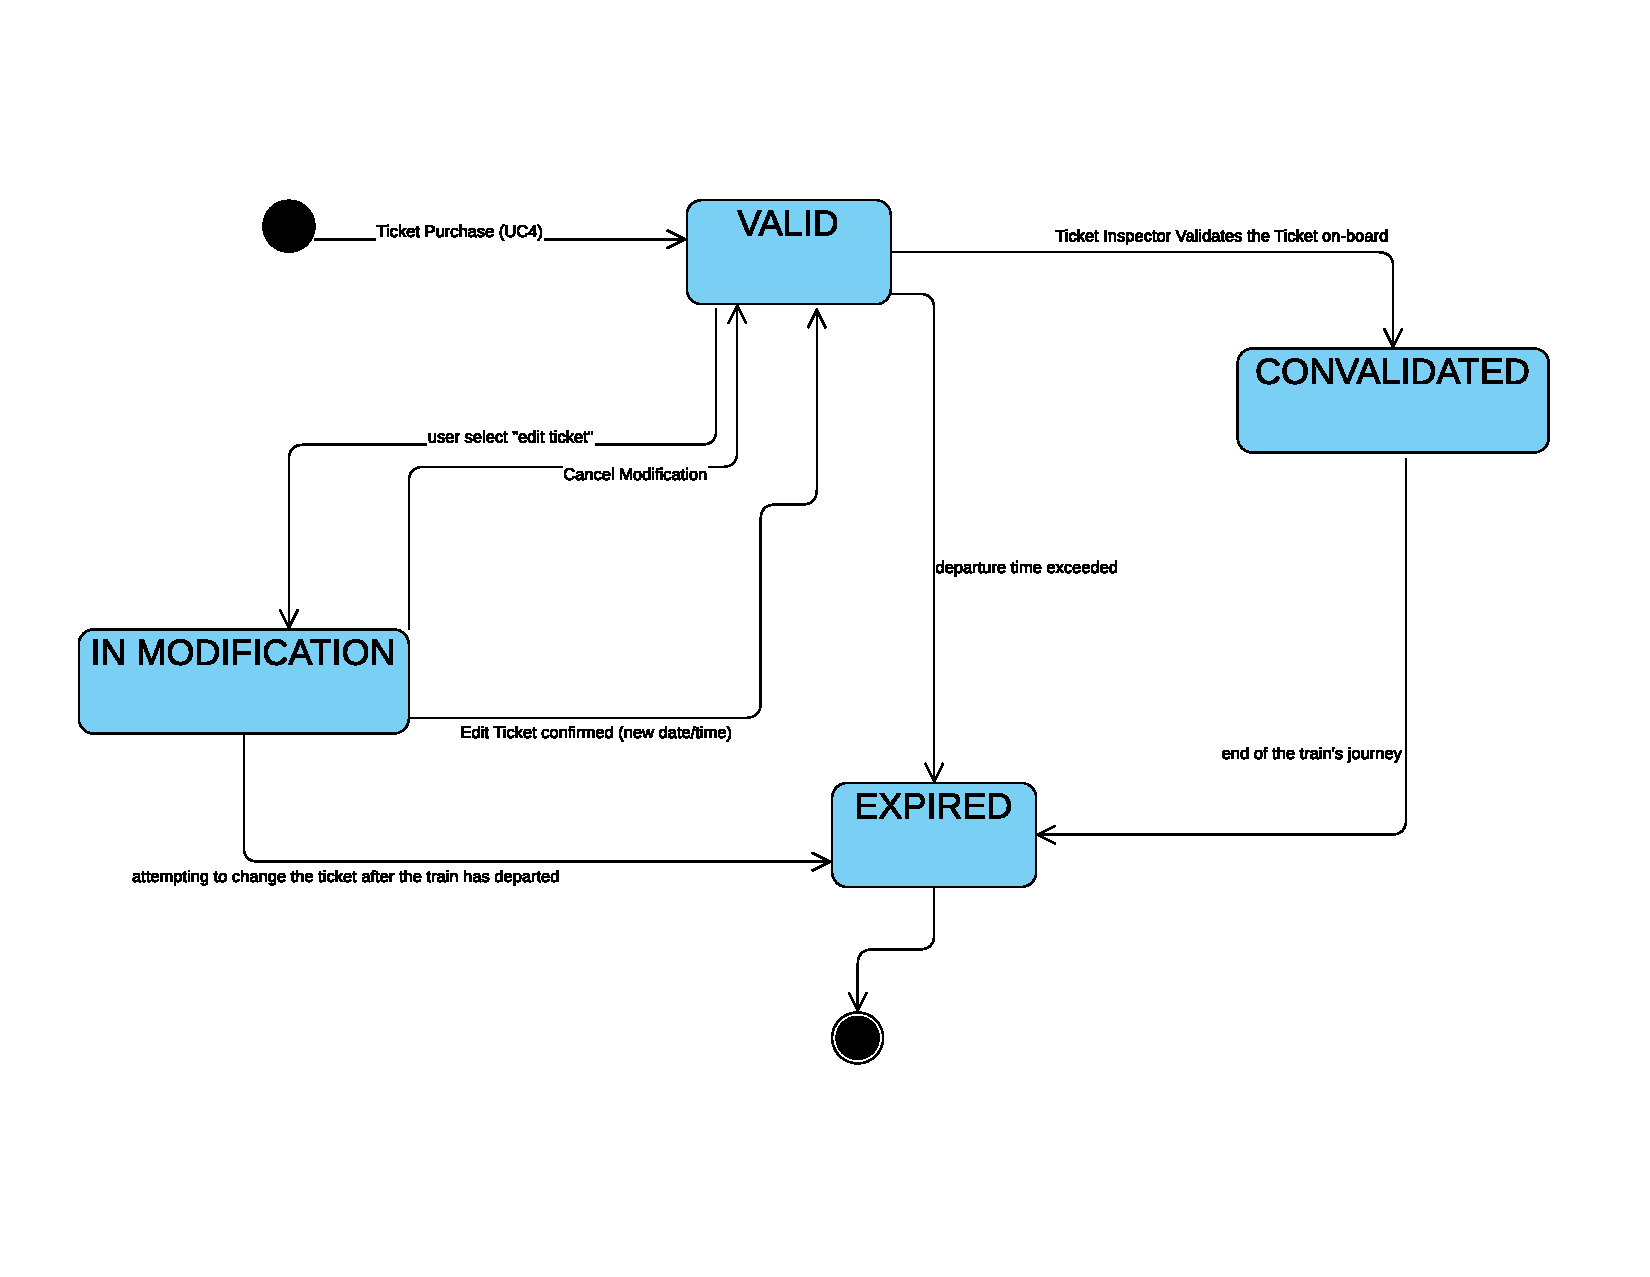
\includegraphics[width=0.9\textwidth]{state-diagram1.pdf}
\end{figure}
\subsection*{Payment-Transaction}
\begin{figure}[H]   
    \centering
    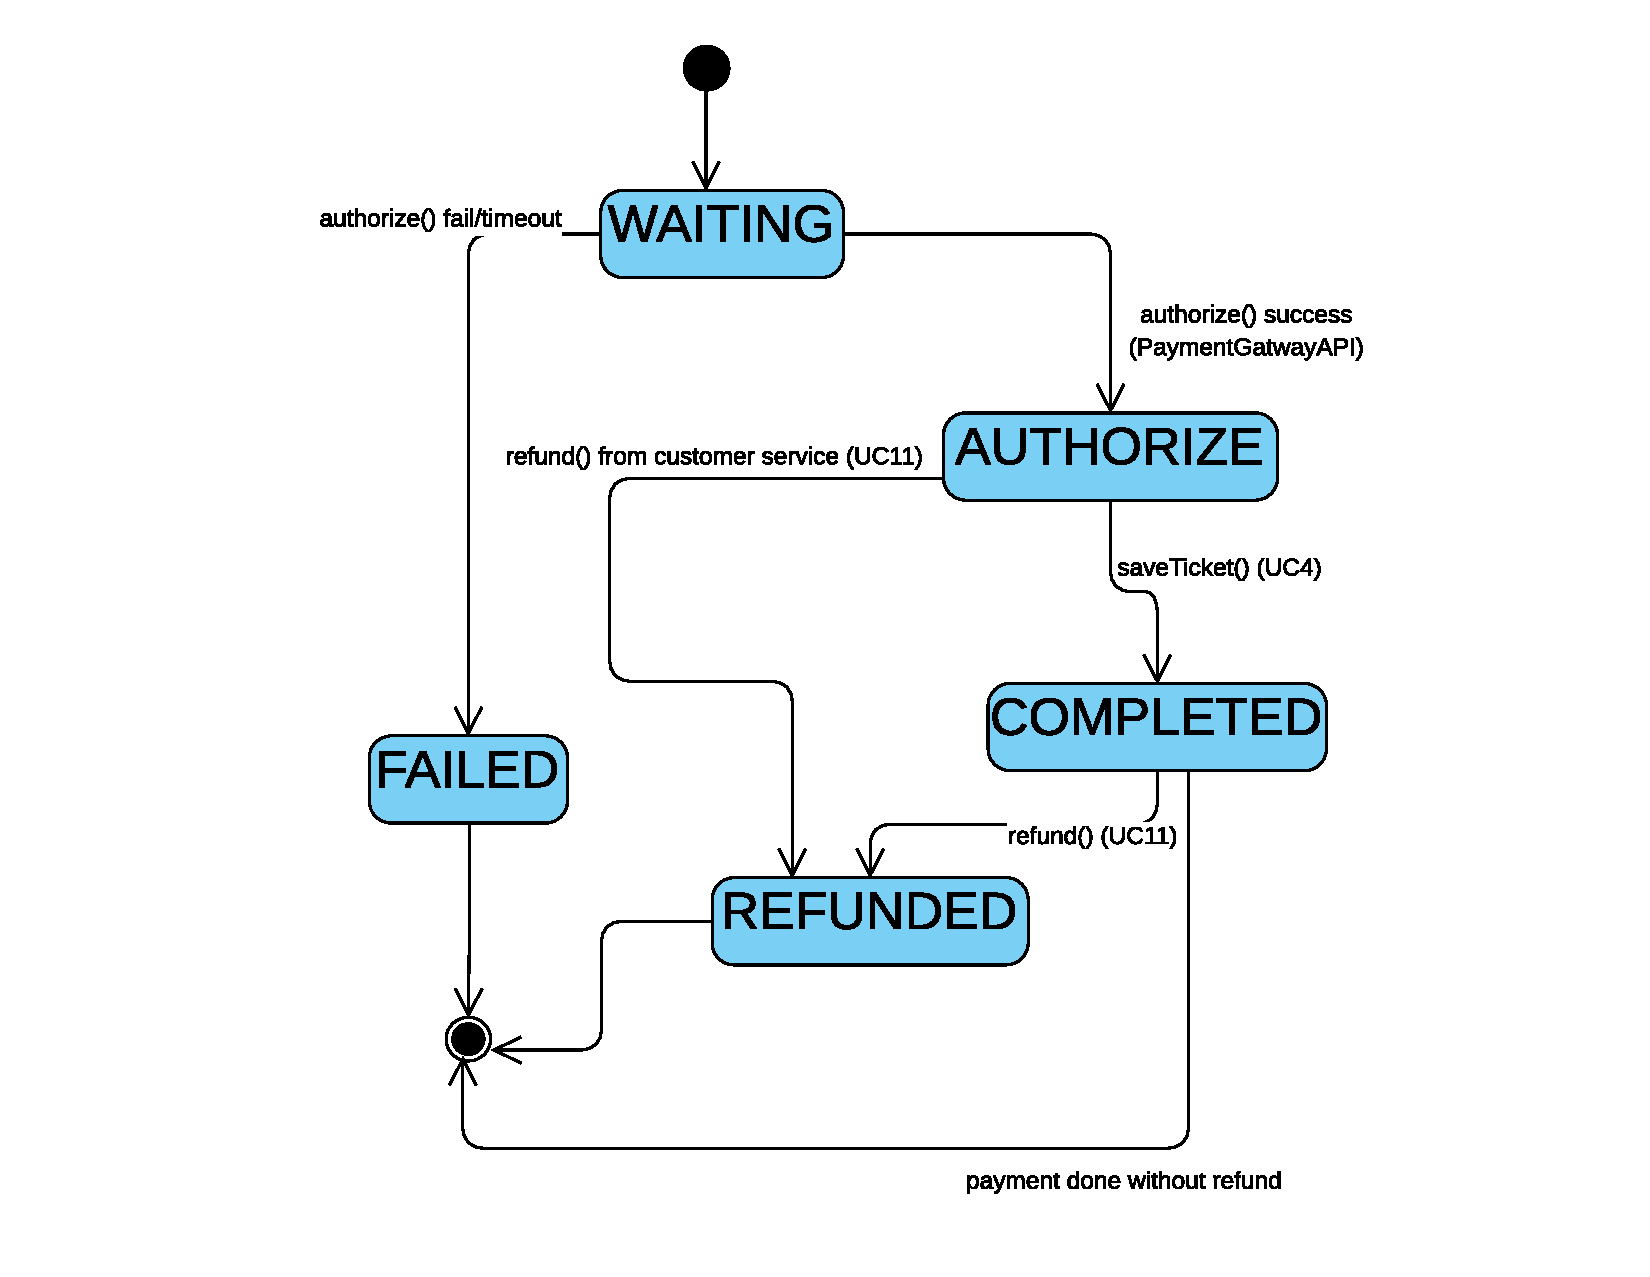
\includegraphics[width=0.7\textwidth]{state-diagram2.pdf}
\end{figure}
\subsection*{User Session}
\begin{figure}[H]   
    \centering
    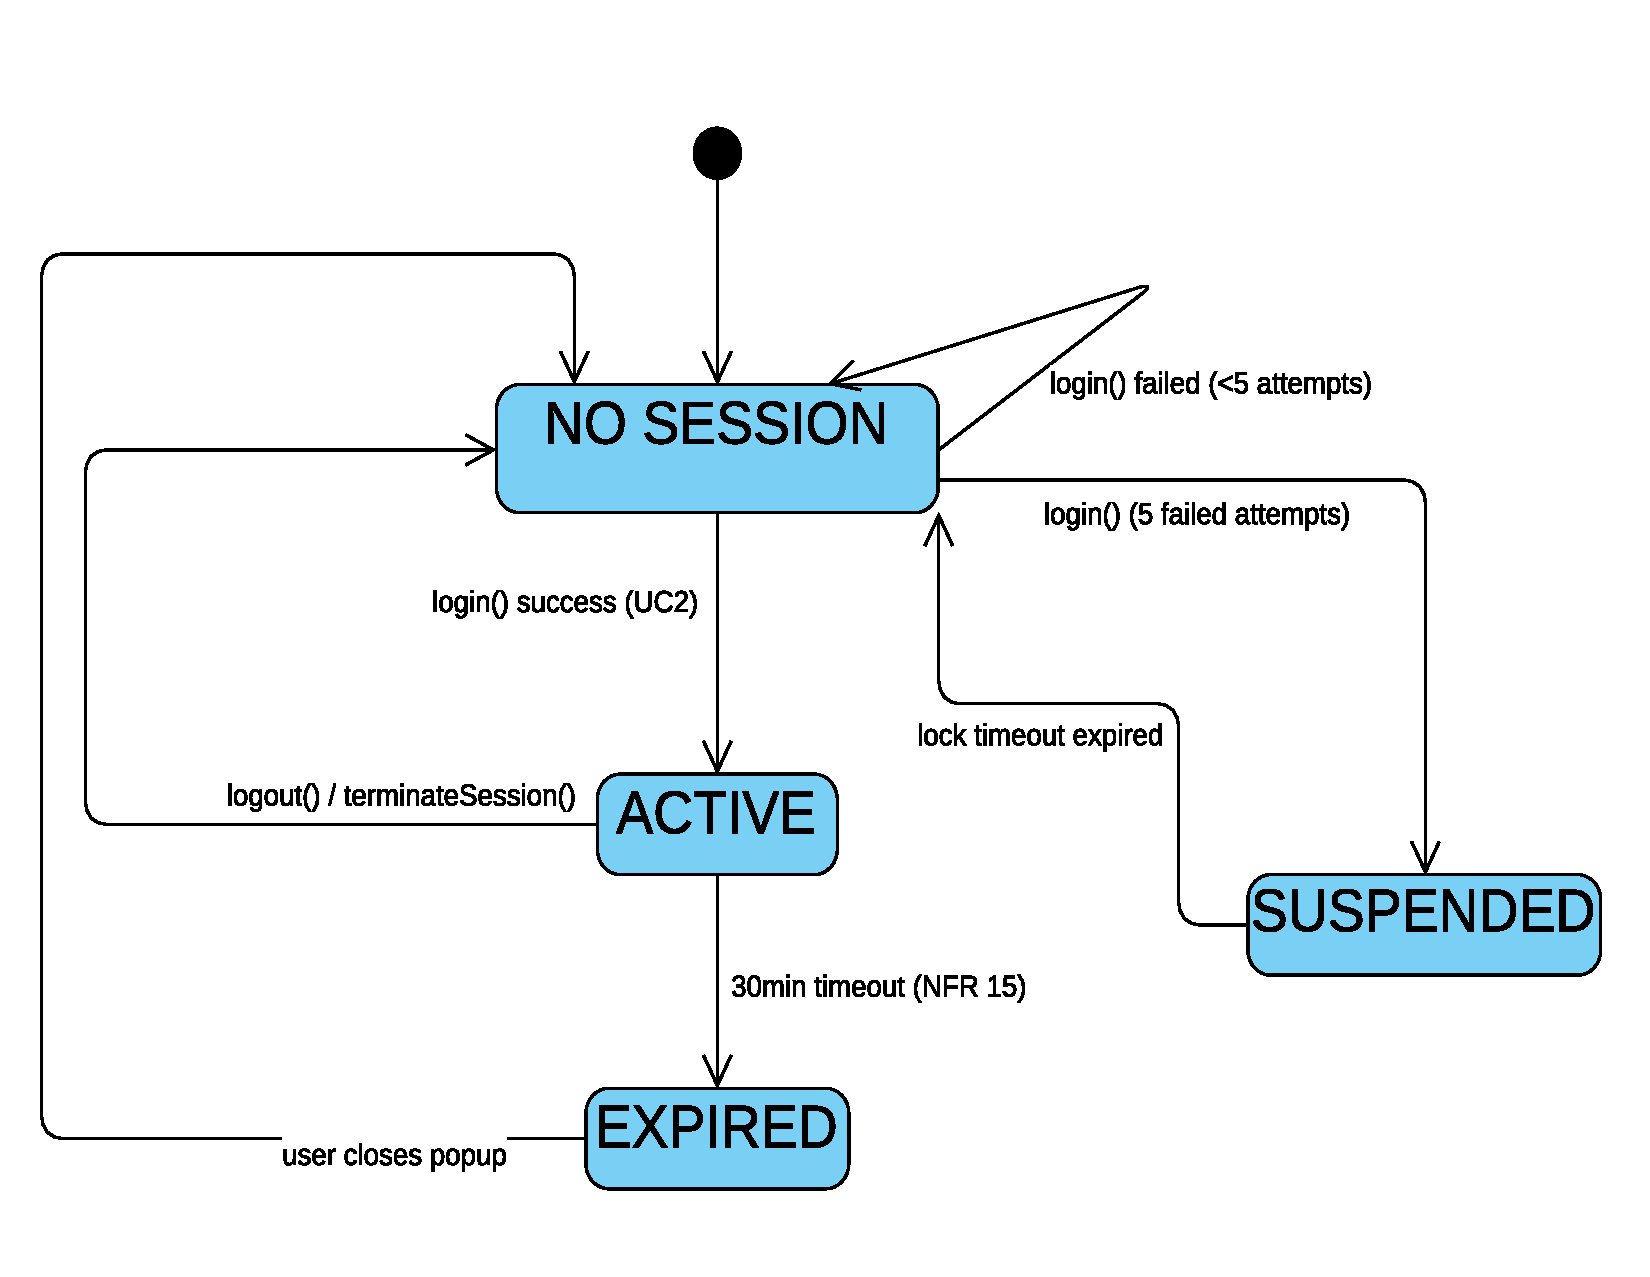
\includegraphics[width=0.7\textwidth]{state-diagram3.pdf}
\end{figure}
\newpage
\begin{landscape}
\section{Class Diagram}
    \vspace*{\fill} % Flexible space at the top
    \begin{center}
        \includegraphics[width=1.5\textwidth]{CLASS-DIAGRAM.pdf}
    \end{center}
    \vspace*{\fill} % Flexible space at the bottom
\end{landscape}
\subsection{Class, Attributes and Methods description}
We will give a brief explanation of some of the principal classes, attributes and methods
% --- ACTORS & USERS ---
\subsubsection*{Class: User (abstract)}
\begin{itemize}
    \item \textbf{Description:} An abstract class that describe a general user 
    \item \textbf{Attributes:}
    \begin{itemize}
        \item \texttt{userId: int}
        \item \texttt{name: String}
        \item \texttt{surname: String}
        \item \texttt{email: String}
        \item \texttt{preferredLanguage: ENUM}
    \end{itemize}
    \item \textbf{Methods:}
    \begin{itemize}
        \item \texttt{changeLanguage(lang: ENUM)}: any user can change the interface language 
    \end{itemize}

    \begin{table}[H]
    \centering
    \begin{tabular}{|>{\columncolor{gray!15}}c|c|}
    \hline
    \rowcolor{gray!30} \textbf{Method} & \textbf{Related Use Case} \\ \hline
    \texttt{changeLanguage()} & UC15: Change Language \\ \hline
    \end{tabular}
    \caption{Method Mapping - User Class}
    \end{table}
    \paragraph{Implementation:} The method of this class is inherited by any user, the preferred language is only saved if the user is registered
\end{itemize}
\subsubsection*{Class: AnonymousUser}
\begin{itemize}
    \item \textbf{Description:} Represents a user not yet registered to the web application.
    \item \textbf{Methods:}
    \begin{itemize}
        \item \texttt{search(criteria:SearchCriteria, mapOpt:Boolean)}: allows the user to insert manually the stations he needs in an apposite section. 
        \item \texttt{selectStation(StationName:String)}: allows the user to select the stations he needs through a map.
        \item \texttt{register(name:String, surname:String, email:String, password:String)}: allows the user to register and create an account. 
    \end{itemize}
    \begin{table}[H]
\centering
\begin{tabular}{|>{\columncolor{gray!15}}c|c|}
\hline
\rowcolor{gray!30} \textbf{Method} & \textbf{Related Use Case} \\ \hline
\texttt{search(criteria:SearchCriteria, mapOpt:Boolean)} & UC1: Search Train \\ \hline
\texttt{selectStation(StationName:String)} & UC1: Search Train \\ \hline
\texttt{register(name:String, surname:String, email:String, password:String)} & UC2: Authentication \\ \hline
\end{tabular}
\caption{Method Mapping - AnonymousUser Class}
\end{table}
\paragraph{Implementation:} searching for a train is allowed also for anonymous users but the registration is requested to continue the purchase.
\end{itemize}

\subsubsection*{Class: RegisteredUser}
\begin{itemize}
    \item \textbf{Description:} Represents a user already registered to the web application and so has a personal account.
    \item \textbf{Attributes:}
    \begin{itemize}
        \item \texttt{passwordHash: String}
        \item \texttt{accountStatus: AccountStatus}
        \item \texttt{failedLoginAttempts: int}
    \end{itemize}
    \item \textbf{Methods:}
    \begin{itemize}
        \item \texttt{login(email:String, password:String)}: allows the registered user to log in his account.
        \item \texttt{logout()}: allows the registered user to log out his account.
        \item \texttt{changePassword(oldPass:String, newPass:String)}: allows the registered user to change his password.
        \item \texttt{requestPasswordRecovery(email:String)}: allows the registered user to recover his password contacting the customer support.
        \item \texttt{eliminateAccount()}: allows the registered user to delete his account (even with active bookings) and be forgotten by the web application.
        \item \texttt{viewActiveDocuments()}: allows registered user to view his active tickets/subscriptions. 
    \end{itemize}
\end{itemize}
\begin{table}[H]
    \centering
    \begin{tabular}{|>{\columncolor{gray!15}}c|c|}
        \hline
        \rowcolor{gray!30} \textbf{Method} & \textbf{Related Use Case} \\ \hline
        \texttt{login() / logout()} & UC2: Authentication \\
        \hline
        \texttt{changePassword(oldPass:String, newPass:String)} & UC10: Account Management \\
        \hline
        \texttt{requestPasswordRecovery(email:String)} & UC10: Account Management \\ \hline
        \texttt{eliminateAccount()} & UC10: Account Management \\
        \hline
        \texttt{viewActiveDocuments()} & UC8: User Dashboard/Profile / UC9: Ticket Management \\ \hline
    \end{tabular}
    \caption{Method Mapping - RegisteredUser Class}
\end{table}
\paragraph{Implementation:} This class includes also customer support agents and ticket inspectors with their own accounts.
\newpage
\subsubsection*{Class: Route}
\begin{itemize}
    \item \textbf{Description:} This class contains the data of the route each train takes.
    \item \textbf{Attributes:}
    \begin{itemize}

    \item \texttt{routeId : int}
    \item \texttt{routeName : String}

    \end{itemize}
    
    \item \textbf{Methods:}
    \begin{itemize}
        \item \texttt{calculateDuration()}: This method computes the total duration of the route considering all scheduled stops.
    \end{itemize}

    \begin{table}[H]
    \centering
    \begin{tabular}{|>{\columncolor{gray!15}}c|c|}
    \hline
    \rowcolor{gray!30} \textbf{Method} & \textbf{Related Use Case} \\ \hline
    \texttt{calculateDuration()} & UC1: Search Train \\ \hline
    \end{tabular}
    \caption{Method Mapping - Route Class}
    \end{table}

    \paragraph{Implementation:} This class models the sequence of stations and intermediate stops that compose a railway journey it aggregates multiple \texttt{Stop} objects.
\end{itemize}

\subsubsection*{Class: Passenger}
\begin{itemize}
    \item \textbf{Description:} Represents a registered user that has already purchased tickets/subscriptions through the web application and took at least one train.
    \item \textbf{Attributes:}
    \begin{itemize}
        \item \texttt{loyaltyPoints: int}
    \end{itemize}
    \item \textbf{Methods:}
    \begin{itemize}
        \item \texttt{selectTrainOptions(criteria: SearchCriteria)}: allows the passenger to select a specific train depending on his necessities while purchasing a ticket (regional, intercity or freccia)
        \item \texttt{confirmPayment(details: PaymentDetails)}: allows the passenger to confirm a transaction when purchasing tickets/subscriptions.
        \item \texttt{selectTicketModify(ticketId: int)}: allows the passenger to select the "Modify Ticket" from his active tickets view and depending on the time left to departure can change date+time (>24h) or only time (<=24h).
        \item \texttt{confirmChange(newDetails: TicketChangeRequest)}: allows the passenger to confirm the changes made on the purchased ticket and update the database.
        \item \texttt{requestTrainStatus(trainId: int)}: allows the passenger to request the real-time train status to check if there is a delay.
        \item \texttt{contactCustomerService(text: string)}: allows the passenger to contact the customer service to clear some doubts or request refunds.
        \item \texttt{viewBookingHistory()}: allows the passeger to view past purchases details in his profile.
        \item \texttt{viewLoyaltyPointsBalance()}: allows the passenger to check updated loyalty points balance in his profile.
    \end{itemize}
    \begin{table}[H]
\centering
\begin{tabular}{|>{\columncolor{gray!15}}c|c|}
\hline
\rowcolor{gray!30} \textbf{Method} & \textbf{Related Use Case} \\ \hline
\texttt{selectTrainOptions(criteria:SearchCriteria)} & UC1: Search Train \\ 
\hline \texttt{confirmPayment(details:PaymentDetails)} & UC4: Purchase \\
\hline \texttt{selectTicketModify(ticketId:int)} & UC9: Ticket Management \\ 
\hline \texttt{confirmChange(newDetails:TicketChangeRequest)} & UC9: Ticket Management \\
\hline \texttt{requestTrainStatus(trainId:int)} & UC5: Check Train Status \\ \hline
\texttt{contactCustomerService(text:String)} & UC11: Customer Support \\ \hline
\texttt{viewBookingHistory()} & UC8: User Dashboard/Profile \\ 
\hline \texttt{viewLoyaltyPointsBalance()} & UC8: User DashBoard/Profile \\
\hline
\end{tabular}
\caption{Method Mapping - Passenger Class}
\end{table}
\paragraph{Implementation:} Confirming the payment the user allows the system to update the loyalty points balance in the dashboard.
\end{itemize}

\subsubsection*{Class: TicketInspector}
\begin{itemize}
    \item \textbf{Description:} Represents the person responsible of checking tickets/subscriptions on the train.
    \item \textbf{Attributes:}
    \begin{itemize}
        \item \texttt{inspectorCode: String}
    \end{itemize}
    \item \textbf{Methods:}
    \begin{itemize}
        \item \texttt{accessSystem()}: allows the ticket inspector to access the system to input data directly.
        \item \texttt{selectValidation()}: allows the ticket inspector to validate passengers' tickets through the system.
        \item \texttt{manualInput(ticketId:int)}: allows the ticket inspector to manually input data in the system.
        \item \texttt{ticketData(ticketId:int)}: allows the ticket inspector to upload data of passengers' tickets on the system. 
        \item \texttt{selectTrackOccupancy()}: allows the ticket inspector to report the track occupancy for making statistics and improve the service.
        \item \texttt{updateOccupancy(coachNumber:int, nPassengers:int)}: allows the ticket inspector to update the track occupancy on the system.
        \item \texttt{viewSchedule(inspId:int)}: allows the ticket inspector to view his shift schedule on an apposite section of his profile.
    \end{itemize}
    \begin{table}[H]
\centering
\begin{tabular}{|>{\columncolor{gray!15}}c|c|}
\hline
\rowcolor{gray!30} \textbf{Method} & \textbf{Related Use Case} \\ \hline
\texttt{accessSystem()} & UC12: Inspector Operations\\ 
\hline \texttt{selectValidation()} & UC12: Inspector Operations \\
\hline
\texttt{manualInput(ticketId:int)} & UC12: Inspector Operations \\ 
\hline \texttt{ticketData(ticketId:int)} & UC12: Inspector Operations \\
\hline \texttt{selectTrackOccupancy()} & UC12: Inspector Operations \\
\hline
\texttt{updateOccupancy(coachNumber:int, nPassengers:int)} & UC12: Inspector Operations \\ \hline
\texttt{viewSchedule(inspId:int)} & UC13: Shift Schedule Visualization \\ \hline
\end{tabular}
\caption{Method Mapping - TicketInspector Class}
\end{table}
\paragraph{Implementation:} After the ticket inspector validates and send the ticket data to the system this one cannot be reused.
\end{itemize}

\subsubsection*{Class: CustomerSupportAgent}
\begin{itemize}
    \item \textbf{Description:} Represents a member of the customer support service that is available to help users and ticket inspectors with doubts and refunds.
    \item \textbf{Attributes:}
    \begin{itemize}
        \item \texttt{staffCode: String}
    \end{itemize}
    \item \textbf{Methods:}
    \begin{itemize}
        \item \texttt{viewUserProfile(userId:int)}: allows the customer support agent to view the user profile to help him more efficiently.
        \item \texttt{manageSupportRequest(requestId:int)}: allows the customer support agent to maanage the requests sent.
        \item \texttt{viewLoyaltyPointsBalance(userId:int)}: allows the customer support agent to view the user's loyalty points balance to elaborate discount packages and offers.
        \item \texttt{viewSchedule(staffId:int)}: allows the customer support agent to view his shift schedule.
    \end{itemize}

    \begin{table}[H]
    \centering
    \begin{tabular}{|>{\columncolor{gray!15}}c|c|}
    \hline
    \rowcolor{gray!30} \textbf{Method} & \textbf{Related Use Case} \\ \hline
    \texttt{viewUserProfile(userId:int)} & UC11: Customer Support \\ \hline
    \texttt{manageSupportRequest(requestId:int)} & UC11: Customer Support \\ \hline
    \texttt{viewLoyaltyPointsBalance(userId:int)} & UC11: Customer Support \\ \hline
    \texttt{viewSchedule(staffId:int)} & UC13: Shift Schedule Visualization/ UC11: Customer Support\\ \hline
    \end{tabular}
    \caption{Method Mapping - CustomerSupportAgent Class}
    \end{table}  
\end{itemize}

\subsubsection*{Class: RailwayAdministrator}
\begin{itemize}
    \item \textbf{Description:} Class that represent the RailwayAdministrator, which is a user that can visualize data and statistics about the train company.
    \item \textbf{Attributes:}
    \begin{itemize}
        \item \texttt{adminCode: String}
    \end{itemize}
    \item \textbf{Methods:}
    \begin{itemize}
        \item \texttt{requestAdminArea()}: allows the administrator to request the access to the admin area.
        \item \texttt{loadStatistics()}: allows the administrator to load the statistics of the company.
        \item \texttt{applyFilters(date: Date, trainLine: String)}: allows the administartor to apply filters.
        \item \texttt{viewStatistics()}: allows the administrator to view statistics of the company.
    \end{itemize}
    \begin{table}[H]
\centering
\begin{tabular}{|>{\columncolor{gray!15}}c|c|}
\hline
\rowcolor{gray!30} \textbf{Method} & \textbf{Related Use Case} \\ \hline
\texttt{requestAdminArea()} & UC3: Admin Area Access \\ \hline
\texttt{loadStatistics()} & UC14: Statistics Visualization \\ 
\hline \texttt{viewStatistics()} & UC14: Statistics Visualization\\
\hline
\texttt{applyFilters(date:Date, trainLine:String)} & UC14: Statistics Visualization \\ \hline
\end{tabular}
\caption{Method Mapping - RailwayAdministrator Class}
\end{table}
\paragraph{Implementation:} This class contains all the actions the Admin can perform.
\end{itemize}

% --- CORE ENTITIES & TRANSACTIONS ---

\subsubsection*{Class: TravelDocument (Abstract)}
\begin{itemize}
    \item \textbf{Description:} Represents the abstract summary of a purchased ticket /subscription indicating its details.
    \item \textbf{Attributes:}
    \begin{itemize}
        \item \texttt{documentId: int}
        \item \texttt{issueDate: DateTime}
        \item \texttt{price: double}
        \item \texttt{status: DocumentStatus}
        \item \texttt{qrCode: String}
    \end{itemize}
    \item \textbf{Methods:}
    \begin{itemize}
        \item \texttt{validate()}: indicates the action of validating the travel document.
        \item \texttt{isActive(currentDate:DateTime)}: indicates if the travel document is valid at current time. 
    \end{itemize}

    \begin{table}[H]
    \centering
    \begin{tabular}{|>{\columncolor{gray!15}}c|c|}
    \hline
    \rowcolor{gray!30} \textbf{Method} & \textbf{Related Use Case} \\ \hline
    \texttt{validate()} & UC12: Inspector Operations \\ \hline
    \texttt{isActive()} & UC9: Ticket Management / UC12: Inspector Operations \\ \hline
    \end{tabular}
    \caption{Method Mapping - TravelDocument Class}
    \end{table}
    \paragraph{Implementation:} The action of validating through the qr code is made by the ticket inspector.
\end{itemize}

\subsubsection*{Class: Ticket}
\begin{itemize}
    \item \textbf{Description:} Represents the digital confirmation of the registered user's purchased ticket that has to be shown to the ticket inspector and includes all the details of the journey (travel document).
    \item \textbf{Attributes:}
    \begin{itemize}
        \item \texttt{ticketId: int}
        \item \texttt{departureTime: DateTime}
        \item \texttt{arrivalTime: DateTime}
        \item \texttt{passengerType: PassengerType}
    \end{itemize}
    \item \textbf{Methods:}
    \begin{itemize}
        \item \texttt{calculateTimeRemaining(currentTime:DateTime)}: allows the system to calculate the time remaining to the departure (CurrentTime vs DepartureTime) to know if it more or less than 24h or if the ticket is already expired.
        \item \texttt{allowFullModification()}: allows the user to change both date and time of departure of an already purchased ticket (only if there are more that 24 hours left to departure).
        \item \texttt{restrictToTimeOnly()}: allows the user to change only the time of departure of an already purchased ticket (in case there are less than 24 hours left to departure).
        \item \texttt{updateTicket(newDetails:TicketChangeRequest)}: allows the system to update the ticket in the database after possible changes.
    \end{itemize}
    \begin{table}[H]
\centering
\begin{tabular}{|>{\columncolor{gray!15}}c|c|}
\hline
\rowcolor{gray!30} \textbf{Method} & \textbf{Related Use Case} \\ \hline
\texttt{calculateTimeRemaining()} & UC9: Ticket Management \\ \hline
\texttt{allowFullModification()} & UC9: Ticket Management \\ \hline
\texttt{restrictToTimeOnly()} & UC9: Ticket Management \\ \hline
\texttt{updateTicket()} & UC9: Ticket Management \\ \hline
\end{tabular}
\caption{Method Mapping - Ticket Class}
\end{table}
\paragraph{Implementation:} The calculateTimeRemaining() method is the one that states if the modification can be full or only partial.
\end{itemize}

\subsubsection*{Class: Subscription}
\begin{itemize}
    \item \textbf{Description:} Represents the digital confirmation of the registered user's purchased subscription that has to be shown to the ticket inspector and includes all the details of the journey (travel document).
    \item \textbf{Attributes:}
    \begin{itemize}
        \item \texttt{subscriptionId: int}
        \item \texttt{startDate: Date}
        \item \texttt{endDate: Date}
        \item \texttt{durationDays: int}
    \end{itemize}
    \item \textbf{Methods:}
    \begin{itemize}
        \item \texttt{renew(durationDays:int)}: allows the user to renew a subscription that has expired.
    \end{itemize}
    \begin{table}[H]
\centering
\begin{tabular}{|>{\columncolor{gray!15}}c|c|}
\hline
\rowcolor{gray!30} \textbf{Method} & \textbf{Related Use Case} \\ \hline
\texttt{renew(durationDays: int)} & UC4:Management Purchase \\ \hline
\end{tabular}
\caption{Method Mapping - Ticket Class}
\end{table}
\end{itemize}

\subsubsection*{Class: Coach}
\begin{itemize}
    \item \textbf{Description:} Represents a section of the train.
    \item \textbf{Attributes:}
    \begin{itemize}
        \item \texttt{coachNumber: int}
        \item \texttt{coachClass: TravelClass}
        \item \texttt{maxPassengers: int}
        \item \texttt{currentPassengers: int}
    \end{itemize}
    \item \textbf{Methods:}
    \begin{itemize}
        \item \texttt{updateOccupancy(nPassengers:int)}: allows the system to indicate the seat taken thanks to the ticket inspector work.
    \end{itemize}
    \begin{table}[H]
\centering
\begin{tabular}{|>{\columncolor{gray!15}}c|c|}
\hline
\rowcolor{gray!30} \textbf{Method} & \textbf{Related Use Case} \\ \hline
\texttt{updateOccupancy(nPassengers:int)} & UC12: Inspector Operations \\ \hline
\end{tabular}
\caption{Method Mapping - AdditionalReservation Class}
\end{table}
\end{itemize}


\subsubsection*{Class: AdditionalReservation (Abstract)}
\begin{itemize}
    \item \textbf{Description:} Represents the possibiity for registered user to add a reservation to his purchase for bikes or lugguages.
    \item \textbf{Attributes:}
    \begin{itemize}
        \item \texttt{reservationId: int}
        \item \texttt{status: ReservationStatus}
        \item \texttt{price: double}
    \end{itemize}
    \item \textbf{Methods:}
    \begin{itemize}
        \item \texttt{confirmReservation()}: allows the registered user to confirm the reservation.
        \item \texttt{cancelReservation()}: allows the registere user to cancel the reservation.
    \end{itemize}
    \begin{table}[H]
\centering
\begin{tabular}{|>{\columncolor{gray!15}}c|c|}
\hline
\rowcolor{gray!30} \textbf{Method} & \textbf{Related Use Case} \\ \hline
\texttt{confirmReservation()} & UC4: Purchase \\ \hline
\texttt{cancelReservation()} & UC9: Ticket Management \\ \hline
\end{tabular}
\caption{Method Mapping - AdditionalReservation Class}
\end{table}
\paragraph{Implementation:} This class is abstract so every type of additional reservation (bikes, lugguages) have the same attributes.
\end{itemize}

\subsubsection*{Class: PaymentTransaction}
\begin{itemize}
    \item \textbf{Description:} Represents the transaction made by the payment system when a ticket/subscription is purchased.
    \item \textbf{Attributes:}
    \begin{itemize}
        \item \texttt{paymentId: int}
        \item \texttt{amount: double}
        \item \texttt{paymentDate: DateTime}
        \item \texttt{paymentStatus: PaymentStatus}
    \end{itemize}
    \item \textbf{Methods:}
    \begin{itemize}
        \item \texttt{authorize(amount:double)}: allows the system to authorize the payment.
        \item \texttt{refund(amount:double)}: allows the system to refund a user after the customer support service has been contacted by a passenger or ticket inspector. 
    \end{itemize}
    \begin{table}[H]
\centering
\begin{tabular}{|>{\columncolor{gray!15}}c|c|}
\hline
\rowcolor{gray!30} \textbf{Method} & \textbf{Related Use Case} \\ \hline
\texttt{authorize()} & UC4: Purchase \\ \hline
\texttt{refund()} & UC11: Customer Support \\ \hline
\end{tabular}
\caption{Method Mapping - Payment Classes}
\end{table}
\paragraph{Implementation:} If the transaction is not authorized through the specific method, no refunds can be made (prevents fraud). The paymentDate attribute is saved in the user's booking history (dashboard).
\end{itemize}

\subsubsection*{Class: SupportRequest}
\begin{itemize}
    \item \textbf{Description:} Represents the request sent by passengers or ticket inspector to customer support service for doubts and refunds.
    \item \textbf{Attributes:}
    \begin{itemize}
        \item \texttt{requestId:int}
        \item \texttt{requestType: SupportRequestType}
        \item \texttt{description: String}
        \item \texttt{status: SupportRequestStatus}
        \item \texttt{creationDate: DateTime}
    \end{itemize}
    \item \textbf{Methods:}
    \begin{itemize}
        \item \texttt{submit()}: allows the passenger or ticket inspector to submit a support request to the customer service.
        \item \texttt{refound()}: Starts or manages the refund process connected to the support request. 
    \end{itemize}

    \begin{table}[H]
    \centering
    \begin{tabular}{|>{\columncolor{gray!15}}c|c|}
    \hline
    \rowcolor{gray!30} \textbf{Method} & \textbf{Related Use Case} \\ \hline
    \texttt{submit()} & UC11: Customer Support \\ \hline
    \texttt{close()} & UC11: Customer Support \\ \hline
    \end{tabular}
    \caption{Method Mapping - SupportRequest Class}
    \end{table}
    \paragraph{Implementation:} When the request is submitted the status is indicated as open until the close() method is called.
\end{itemize}

\subsubsection*{Class: Notification}
\begin{itemize}
    \item \textbf{Description:} Represents the information sent to registered users by the web application.
    \item \textbf{Attributes:}
    \begin{itemize}
        \item \texttt{notificationId: int}
        \item \texttt{message: String}
        \item \texttt{notificationDate: DateTime}
        \item \texttt{notificationType: NotificationType}
    \end{itemize}
    \item \textbf{Methods:}
    \begin{itemize}
        \item \texttt{pushInAppAlert()}: indicates the important notifications received by passengers in case of problems or delays of the trains.
        \item \texttt{sendEmailNotification()}: indicates information sent by email to registered users.
    \end{itemize}
    \begin{table}[H]
\centering
\begin{tabular}{|>{\columncolor{gray!15}}c|c|}
\hline
\rowcolor{gray!30} \textbf{Method} & \textbf{Related Use Case} \\ \hline
\texttt{pushInAppAlert()} & UC7: Receive Notifications\\
\hline \texttt{sendEmailNotification()} & UC7: Receive Notifications \\ 
\hline
\end{tabular}
\caption{Method Mapping - Notification Class}
\end{table}
\paragraph{Implementation:} This class is redundant as in case of urgency both methods are activated so the user receive two notifications on different apps.
\end{itemize}

% --- DOMAIN / TRAIN ENTITIES ---

\subsubsection*{Class: StationBoard}
\begin{itemize}
    \item \textbf{Description:} This class is used to display the arrival/departure board of each station
    \item \textbf{Attributes:}
    \begin{itemize}

    \item \texttt{boardId : int}
    \item \texttt{boardType : BoardType}
    \item \texttt{lastUpdate : DateTime}

    \end{itemize}
    \item \textbf{Methods:}
    \begin{itemize}
        \item \texttt{updateDisplay()}: used to update every time a new entry, from the class \texttt{BoardEntry} is present the board of trains
    \end{itemize}
    \begin{table}[H]
\centering
\begin{tabular}{|>{\columncolor{gray!15}}c|c|}
\hline
\rowcolor{gray!30} \textbf{Method} & \textbf{Related Use Case} \\ \hline
\texttt{updateDisplay()} & UC6: Boards Visualization \\ \hline
\end{tabular}
\caption{Method Mapping - Real-time Display Classes}
\end{table}
\paragraph{Implementation:} This class is part of the structure of the railway network. \texttt{StationBoard} acts as the data structure for the public board.
\end{itemize}

\subsubsection*{Class: Seat}
\begin{itemize}
    \item \textbf{Description:} This class describes how we handle seat, is part of class \texttt{Coach}, ad it can be reserved or mark occupied from the Ticket Inspector to update occupancy 
    \item \textbf{Attributes:}
    \begin{itemize}

    \item \texttt{seatNumber : String}
    \item \texttt{seatStatus : SeatStatus}
    \end{itemize}
    \item \textbf{Methods:}
    \begin{itemize}
        \item \texttt{reserve()}: when buying a ticket the system reserves a seat (only on train type where is possible to book a seat)
        \item \texttt{markOccupied()}: method called when the ticket inspector update to mark the occupancy
    \end{itemize}
    \begin{table}[H]
\centering
\begin{tabular}{|>{\columncolor{gray!15}}c|c|}
\hline
\rowcolor{gray!30} \textbf{Method} & \textbf{Related Use Case} \\ \hline
\texttt{reserve()} & UC4: Purchase \\ \hline
\texttt{markOccupied()} & UC12: Inspector Operations \\ \hline
\end{tabular}
\caption{Method Mapping - Seat Class}
\end{table}
\end{itemize}
\newpage
\subsubsection*{Class: Train}
\begin{itemize}
    \item \textbf{Description:} Represents the vehicle taken by the passengers for their journey and where the train staff works.
    \item \textbf{Attributes:}
    \begin{itemize}
        \item \texttt{trainId: int}
        \item \texttt{trainCode: String}
        \item \texttt{trainType: TrainType}
        \item \texttt{serviceClass: TravelClass}
    \end{itemize}
    \item \textbf{Methods:}
    \begin{itemize}
        \item \texttt{getLiveLocation(trainId:int)}: allows system to get the live location of a specific train.
        \item \texttt{getDelayEstimate(trainId:int)}: allows system to get an estimate of delay of a specific train to show it on boards.
    \end{itemize}

    \begin{table}[H]
    \centering
    \begin{tabular}{|>{\columncolor{gray!15}}c|c|}
    \hline
    \rowcolor{gray!30} \textbf{Method} & \textbf{Related Use Case} \\ \hline
    \texttt{getLiveLocation()} & UC5: Check Train Status \\ \hline
    \texttt{getDelayEstimate()} & UC5: Check Train Status \\ \hline
    \end{tabular}
    \caption{Method Mapping - Train Class}
    \end{table}
    \paragraph{Implementation:} All attributes are static but the two methods give dynamic data.
\end{itemize}

\subsubsection*{Class: TrainOption}
\begin{itemize}
    \item \textbf{Description:} Represents the train option the user chooses.
    \item \textbf{Attributes:}
    \begin{itemize}
        \item \texttt{optionId: int}
        \item \texttt{totalPrice: double}
        \item \texttt{availableSeats: int}
    \end{itemize}
    \item \textbf{Methods:}
    \begin{itemize}
        \item \texttt{displayTotal(): double}: allows the user to see the total price of the train chosen.
    \end{itemize}

    \begin{table}[H]
    \centering
    \begin{tabular}{|>{\columncolor{gray!15}}c|c|}
    \hline
    \rowcolor{gray!30} \textbf{Method} & \textbf{Related Use Case} \\ \hline
    \texttt{displayTotal()} & UC1: Search Train \\ \hline
    \end{tabular}
    \caption{Method Mapping - Train Class}
    \end{table}
\end{itemize}

\subsubsection*{Class: TrainRun}
\begin{itemize}
    \item \textbf{Description:} Represents a specific scheduled run made by a train identified by a runId.
    \item \textbf{Attributes:}
    \begin{itemize}
        \item \texttt{runId: int}
        \item \texttt{departureDate: Date}
        \item \texttt{status: TrainRunStatus}
        \item \texttt{currentDelayMinutes: int}
    \end{itemize}
    \item \textbf{Methods:}
    \begin{itemize}
       \item \texttt{reportDelay(trainId:int, delayTime:int)}: allows the system to report a possible delay of a specific run.
        \item \texttt{refreshData()}: allows the system to update data of every train run shown on boards. 
    \end{itemize}

    \begin{table}[H]
    \centering
    \begin{tabular}{|>{\columncolor{gray!15}}c|c|}
    \hline
    \rowcolor{gray!30} \textbf{Method} & \textbf{Related Use Case} \\ \hline
    \texttt{reportDelay()} & UC5: Check Train Status \\ \hline
    \texttt{refreshData()} & UC5: Check Train Status / UC6: Boards Visualization \\ \hline
    \end{tabular}
    \caption{Method Mapping - TrainRun Class}
    \end{table}
    \paragraph{Implementation:} A train performs multiple runs every day.
\end{itemize}

\subsubsection*{Class: DelayEstimate}
\begin{itemize}
    \item \textbf{Description:} This class handles the prediction of the delay of train runs.
    \item \textbf{Attributes:}
    \begin{itemize}
    \item \texttt{estimateId : int}
    \item \texttt{delayMinutes : int}
    \item \texttt{confidence : double}
    \end{itemize}
    \item \textbf{Methods:}
    \begin{itemize}
        \item \texttt{getDelayPrediction(trainId: int)}: when this method is called is runs some simple ML prediction algorithm to generate a time prediction
    \end{itemize}
    \begin{table}[H]
\centering
\begin{tabular}{|>{\columncolor{gray!15}}c|c|}
\hline
\rowcolor{gray!30} \textbf{Method} & \textbf{Related Use Case} \\ \hline
\texttt{getDelayPrediction()} & UC5: Check Train Status \\ \hline
\end{tabular}
\caption{Method Mapping - Train Status Classes}
\end{table}
\end{itemize}

\subsubsection*{Class: PredictionSystem}
\begin{itemize}
    \item \textbf{Description:} Provides delay estimates for trains.
    \item \textbf{Methods:}
    \begin{itemize}
        \item \texttt{getDelayPrediction(trainIds: String)}: returns delay predictions for a list of trains.
        \item \texttt{getDelayEstimate(trainId: int)}: returns the estimated delay for a specific train.
    \end{itemize}
    \begin{table}[H]
\centering
\begin{tabular}{|>{\columncolor{gray!15}}c|c|}
\hline
\rowcolor{gray!30} \textbf{Method} & \textbf{Related Use Case} \\ \hline
\texttt{getDelayPrediction()} & UC1: Search Train  \\ \hline
\texttt{getDelayEstimate()} & UC5: Check Train Status \\ \hline
\end{tabular}
\caption{Method Mapping - Train Status Classes}
\end{table}
\paragraph{Implementation:} Search and status features call this component when they need delay information. The interface uses its output to show better travel information to the user.
\end{itemize}


% --- SEARCH & SCHEDULING ---

\subsubsection*{Class: SearchCriteria}
\begin{itemize}
    \item \textbf{Description:} Represents the criteria the user has to insert to search for a train. 
    \item \textbf{Attributes:}
    \begin{itemize}
        \item \texttt{departureStationName: String}
        \item \texttt{arrivalStationName: String}
        \item \texttt{date: Date}
        \item \texttt{time: Time}
        \item \texttt{trainType: TrainType}
        \item \texttt{travelClass: TravelClass}
        \item \texttt{passengerCount: int}
    \end{itemize}
    \item \textbf{Methods:}
    \begin{itemize}
        \item \texttt{validate()}: allows the system to check the data inserted make sense and search trains that match them without wasting resources.
    \end{itemize}
    \begin{table}[H]
\centering
\begin{tabular}{|>{\columncolor{gray!15}}c|c|}
\hline
\rowcolor{gray!30} \textbf{Method} & \textbf{Related Use Case} \\ \hline
\texttt{validate()} & UC1: Search Train \\ \hline

\end{tabular}
\caption{Method Mapping - Search Logic Classes}
\end{table}
\paragraph{Implementation:} In case of trips that are in the past or station of departure and arrival being the same the system send feedback to the user.
\end{itemize}

\subsubsection*{Class: TrainSearchResult}
\begin{itemize}
    \item \textbf{Description:} Represents the list and number of results that match the inserted search criteria.
    \item \textbf{Attributes:}
    \begin{itemize}
        \item \texttt{resultId: int}
        \item \texttt{resultCount: int}
    \end{itemize}
    \item \textbf{Methods:}
    \begin{itemize}
        \item \texttt{displayResults(criteria:SearchCriteria)}: allows the system to display the results matching the inserted criteria.
        \item \texttt{applyFilters(criteria:SearchCriteria)}: allows the system to display filters from which the user can choose what to select.
    \end{itemize}
    \begin{table}[H]
\centering
\begin{tabular}{|>{\columncolor{gray!15}}c|c|}
\hline
\rowcolor{gray!30} \textbf{Method} & \textbf{Related Use Case} \\ \hline

\texttt{applyFilters()} & UC1: Search Train \\ \hline
\texttt{}displayResults() & UC1: Search Train \\ \hline
\end{tabular}
\caption{Method Mapping - Search Logic Classes}
\end{table}
\paragraph{Implementation:} Applying filters creates a subset of the results initially displayed. This class is temporary as it is deleted when the user finishes searching.
\end{itemize}


\subsubsection*{Class: StatisticsReport}
\begin{itemize}
    \item \textbf{Description:} Represents a report generated from the system statistics.
    \item \textbf{Attributes:}
    \begin{itemize}
        \item \texttt{reportId: int}
        \item \texttt{reportType: string}
        \item \texttt{generationDate: DateTime}
    \end{itemize}
    \item \textbf{Methods:}
    \begin{itemize}
        \item \texttt{applyFilters(filters: StatistricsFilter)}
        \item \texttt{displayData()}
    \end{itemize}
    \begin{table}[H]
\centering
\begin{tabular}{|>{\columncolor{gray!15}}c|c|}
\hline
\rowcolor{gray!30} \textbf{Method} & \textbf{Related Use Case} \\ \hline
\texttt{applyFilters() / displayData()} & UC14: Statistics Visualization \\ \hline
\end{tabular}
\caption{Method Mapping - StatisticsReport Class}
\end{table}
\end{itemize}

\subsubsection*{Class: TicketChangeRequest}
\begin{itemize}
    \item \textbf{Description:} Represents the request from a passenger to modify an already purchased ticket.
    \item \textbf{Attributes:}
    \begin{itemize}
        \item \texttt{newDate: Date}
        \item \texttt{newTime: Time}
        \item \texttt{changeType: ChangeType}
    \end{itemize}
    \item \textbf{Methods:}
    \begin{itemize}
        \item \texttt{validateAgainstThreshold(departureTime:DateTime)}: allows the system to analyze if the ticket can be modify in both date and time of departure or only time based on the hours left to expiration (more or less/equal than 24 hours)
    \end{itemize}
    \begin{table}[H]
\centering
\begin{tabular}{|>{\columncolor{gray!15}}c|c|}
\hline
\rowcolor{gray!30} \textbf{Method} & \textbf{Related Use Case} \\ \hline
\texttt{validateAgainstThreshold()} & UC9: Ticket Management \\ \hline
\end{tabular}
\caption{Method Mapping - TicketChangeRequest Class}
\end{table}
\paragraph{Implementation:} This class indicates the policy behind the process of refund request.
\end{itemize}
\newpage
\subsubsection*{Class: PaymentDetails}
\begin{itemize}
    \item \textbf{Description:} Contains the basic information needed to start a payment: the payment method chosen by the user and the temporary transaction reference used during the checkout.
        \item \textbf{Attributes:}
    \begin{itemize}
        \item \texttt{paymentMethod: string}
        \item \texttt{tokenizedReference: string}
    \end{itemize}
    \item \textbf{Methods:}
    \begin{itemize}
        \item \texttt{validate()}: checks if the payment information are complete and can be sent to the payment system.
        
    \end{itemize}
    \begin{table}[H]
\centering
\begin{tabular}{|>{\columncolor{gray!15}}c|c|}
\hline
\rowcolor{gray!30} \textbf{Method} & \textbf{Related Use Case} \\ \hline
\texttt{validate()} & UC4: Purchase \\ \hline
\end{tabular}
\caption{Method Mapping - Payment Classes}
\end{table}
\paragraph{Implementation:} This class is used as a simple data object during the purchase process. It does not directly execute the payment, but it provides the data needed by the \texttt{TicketPurchaseController} and by the external \texttt{PaymentGatewayAPI}.
\end{itemize}

\subsubsection*{Class: PaymentResult}
\begin{itemize}
    \item \textbf{Description:} Represents the outcome of a payment request. It stores whether the payment was accepted or rejected, the transaction code returned by the payment system, and a message that can be shown to the user.
    \item \textbf{Attributes:}
    \begin{itemize}
        \item \texttt{authorized: boolean}
        \item \texttt{transactionCode: string}
        \item \texttt{message: string}
    \end{itemize}
\paragraph{Implementation:} This class is used to transfer the result of the payment authorization back to the system. The \texttt{TicketPurchaseController} uses it to decide whether the ticket or subscription can be generated or whether the user must be informed about a failed payment.
\end{itemize}

\subsubsection*{Class: ValidationResult}
\begin{itemize}
    \item \textbf{Description:} Represents the result of a ticket or subscription validation. It stores whether the document is valid or not and an explanation message.
    \item \textbf{Attributes:}
    \begin{itemize}
        \item \texttt{valid: boolean}
        \item \texttt{alreadyValidate: boolean}
        \item \texttt{message: string}
    \end{itemize}
\paragraph{Implementation:} This class is used by the validation workflow to communicate the outcome of a ticket check. It allows the system to handle successful validations, already validated tickets, and invalid documents in a consistent way.
\end{itemize}

\subsubsection*{Class: SessionToken}
\begin{itemize}
    \item \textbf{Description:} Represents the active session of a user. It stores the token value and its expiration time.
    \item \textbf{Attributes:}
    \begin{itemize}
        \item \texttt{tokenvalue: string}
        \item \texttt{expirationTime: dateTime}
    \end{itemize}
    \item \textbf{Methods:} 
    \begin{itemize}
        \item \texttt{isExpired(currentTime: DateTime)}: checks whether the session is still valid at the given time.
    \end{itemize}
    \begin{table}[H]
\centering
\begin{tabular}{|>{\columncolor{gray!15}}c|c|}
\hline
\rowcolor{gray!30} \textbf{Method} & \textbf{Related Use Case} \\ \hline
\texttt{isExpired()} & UC2: Authentication \\ \hline
\end{tabular}
\caption{Method Mapping - Payment Classes}
\end{table}
\paragraph{Implementation:} After a successful login, the system creates one of these and it's used to verify whether a user can continue accessing protected features or must log in again.
\end{itemize}

\subsubsection*{Class: Dashboard}
\begin{itemize}
    \item \textbf{Description:} Represents the admin view used to display statistics and operational information. It contains the data required to show charts, reports, and filtered results.
    \item \textbf{Attributes:}
    \begin{itemize}
        \item \texttt{dashboardId: int}
        \item \texttt{title: string}
    \end{itemize}
\paragraph{Implementation:} This class is used as a presentation object for the administrative area. It receives already processed statistics and makes them available to the interface in a clear and organized way.
\end{itemize}

\subsubsection*{Class: OccupancyPanel}
\begin{itemize}
    \item \textbf{Description:} Represents the interface used by the ticket inspectors to update and monitor train occupancy in real time during their shift.
    \item \textbf{Attributes:}
    \begin{itemize}
        \item \texttt{panelId: int}
    \end{itemize}
\paragraph{Implementation:} This class allows the inspector to update occupancy information during service. The collected data can then be used to show passengers the current crowding level of a train.
\end{itemize}

\subsubsection*{Class: ValidationPanel}
\begin{itemize}
    \item \textbf{Description:} Represents the interface used by the ticket inspectors to validate tickets or subscriptions during their shift.
    \item \textbf{Attributes:}
    \begin{itemize}
        \item \texttt{panelId: int}
    \end{itemize}
\paragraph{Implementation:} This class doesn't validate anything itself. It takes the input, hands it off to the \texttt{ValidationController}, and shows whatever comes back. 
\end{itemize}

\subsubsection*{Class: UserProfile}
\begin{itemize}
    \item \textbf{Description:} Represents the personal area of a registered user. It contains the information needed to access active tickets, subscriptions, booking history, and loyalty points.
    \item \textbf{Attributes:}
    \begin{itemize}
        \item \texttt{profileId: int}
    \end{itemize}
\paragraph{Implementation:} This class supports the dashboard/profile use case. It organizes user-related information and allows the interface to display travel documents, past bookings, and loyalty data.
\end{itemize}

\subsubsection*{Class: TravelDocumentSummary}
\begin{itemize}
    \item \textbf{Description:} Represents a compact view of a user’s active ticket or subscription. It contains only the main information needed to quickly identify and display a travel document.
    \item \textbf{Attributes:}
    \begin{itemize}
        \item \texttt{activeCount: int}
    \end{itemize}
\paragraph{Implementation:} This class is used to show active tickets and subscriptions in the user profile without loading every detailed field of the full travel document.
\end{itemize}

\subsubsection*{Class: BookingHistory}
\begin{itemize}
    \item \textbf{Description:} Represents the list of past purchases made by a registered user. It stores references to previous bookings and can be used to help the user repeat similar searches or purchases.
    \item \textbf{Attributes:}
    \begin{itemize}
        \item \texttt{historyId: int}
    \end{itemize}
\paragraph{Implementation:} This class supports the user profile by collecting past travel records. It can also be used to pre-fill future searches based on previous routes.
\end{itemize}

\subsubsection*{Class: StatisticsFilter}
\begin{itemize}
    \item \textbf{Description:} Holds the criteria used by an admin to filter the statistics dashboard (such as date, train line, and report type).
    \item \textbf{Attributes:}
    \begin{itemize}
        \item \texttt{date: date}
        \item \texttt{trainLine: string}
        \item \texttt{type: string}
    \end{itemize}
\paragraph{Implementation:} This class is used when the admin refines the statistics displayed on the dashboard. It allows the system to request only the relevant data from the database or reporting logic.
\end{itemize}

\subsubsection*{Class: TrainStatus}
\begin{itemize}
    \item \textbf{Description:} Represents the current status of a train (where a train is and how it's doing right now). It contains scheduled and estimated times, current location, delay information, and the delay-warning flag.
    \item \textbf{Attributes:}
    \begin{itemize}
        \item \texttt{scheduledDeparture: dateTime}
        \item \texttt{estimatedDeparture: dateTime}
        \item \texttt{scheduledArrival: dateTime}
        \item \texttt{estimatedArrival: dateTime}
        \item \texttt{delayMinutes: int}
    \end{itemize}
    \item \textbf{Methods:}
    \begin{itemize}
        \item \texttt{displayVisualTimeline(location: Location, delay: DelayEstimate)}: displays the train progress and expected delay in a visual form.
    \end{itemize}
    \begin{table}[H]
    \centering
    \begin{tabular}{|>{\columncolor{gray!15}}c|c|}
    \hline
    \rowcolor{gray!30} \textbf{Method} & \textbf{Related Use Case} \\ \hline
\texttt{displayVisualTimeline()} & UC5: Check Train Status \\ \hline
    \end{tabular}
    \caption{Method Mapping - Stop Class}
    \end{table}

    \paragraph{Implementation:} This class is used to present real-time train information to the user. It adds timetable data, current position, and delay estimates into a object that can be displayed to the user by the interface.
\end{itemize}

\subsubsection*{Class: Stop}
\begin{itemize}
    \item \textbf{Description:} This class represents an intermediate or terminal stop of a train along a route, it contains also timing information. This class must coincide with a station.
    \item \textbf{Attributes:}
    \begin{itemize}

    \item \texttt{stopOrder : int}
    \item \texttt{scheduledArrival : DateTime}
    \item \texttt{scheduledDeparture : DateTime}
    \item \texttt{estimatedArrival : DateTime}
    \item \texttt{estimatedDeparture : DateTime}
    \item \texttt{trackNumber : String}

    \end{itemize}
    \paragraph{Implementation:} This class is used to store every station stop included in a train route. It stores both planned and real-time operational data.
\end{itemize}
\newpage
\subsubsection*{Class: Station}
\begin{itemize}
    \item \textbf{Description:} This class represents a physical railway station in the transportation network. It stores all the data of the station (name, coordinates, city and code).This class may coincide with a stop.
    \item \textbf{Attributes:}
    \begin{itemize}

    \item \texttt{stationId : int}
    \item \texttt{name : String}
    \item \texttt{city : String}
    \item \texttt{code : String}

    \end{itemize}

    \item \textbf{Methods:}
    \begin{itemize}
        \item \texttt{displayBoard(data: StationBoard)}: Flags when there is a need to displays the live departure/arrival board at the selected station.
    \end{itemize}

    \begin{table}[H]
    \centering
    \begin{tabular}{|>{\columncolor{gray!15}}c|c|}
    \hline
    \rowcolor{gray!30} \textbf{Method} & \textbf{Related Use Case} \\ \hline
    \texttt{displayBoard()} & UC6: Boards Visualization \\ \hline
    \end{tabular}
    \caption{Method Mapping - Station Class}
    \end{table}

    \paragraph{Implementation:} This class collaborates with the \texttt{StationBoard} entity to provide real-time information about departures and arrivals.
\end{itemize}
\subsubsection*{Class: BoardEntry}
\begin{itemize}
    \item \textbf{Description:} This class represents a single row inside a departure/arrival board, containing train timing, platform, and status information.
    \item \textbf{Attributes:}
    \begin{itemize}
    \item \texttt{scheduledTime : DateTime}
    \item \texttt{estimatedTime : DateTime}
    \item \texttt{platform : String}
    \item \texttt{entryStatus : BoardEntryStatus}
    \end{itemize}
\end{itemize}

% --- CONTROLLERS ---

\subsubsection*{Class: TicketManagementController}
\begin{itemize}
    \item \textbf{Description:} Manages the process of modifying an already purchased ticket. 
    \item \textbf{Methods:}
    \begin{itemize}
        \item \texttt{selectTicketModify(ticketId: int)}: Selects the ticket that the user wants to modify.
        \item \texttt{requestModification(ticketId: int)}: Starts the modification request for a specific ticket. 
        \item \texttt{getTicketDetails(ticketId: int)}
        \item \texttt{calculateTimeRemaining(departureTime: DateTime)}: Calculates how much time is left before the train departure.
        \item \texttt{allowFullModification()}: Checks whether the ticket can be fully modified. 
        \item \texttt{restrictToTimeOnly()}:  Applies the restriction that allows the user to change only the departure time and not the date. 
        \item \texttt{confirmChange(newDetails: TicketChangeRequest)}
        \item \texttt{updateTicket(ticketId: int, newDetails: TicketChangeRequest)}
        \item \texttt{showErrorMessage(message: String)}:  Displays an error message when the modification cannot be completed. 
    \end{itemize}
    \begin{table}[H]
\centering
\begin{tabular}{|>{\columncolor{gray!15}}c|c|}
\hline
\rowcolor{gray!30} \textbf{Method} & \textbf{Related Use Case} \\ \hline
\texttt{requestModification() / confirmChange()} & UC9: Ticket Management \\ \hline
\texttt{calculateTimeRemaining()} & UC9: Ticket Management \\ \hline
\texttt{updateTicket() / showErrorMessage()} & UC9: Ticket Management \\ \hline
\end{tabular}
\caption{Method Mapping - TicketManagementController Class}
\end{table}

\end{itemize}

\subsubsection*{Class: TrainSearchController}
\begin{itemize}
    \item \textbf{Description:} Manages train search operations. It receives a search request and turns it into a list of travel options.
    \item \textbf{Methods:}
    \begin{itemize}
        \item \texttt{search(criteria: SearchCriteria, mapOpt: Boolean)}: starts the train search using normal input or map-based station selection.
        \item \texttt{resolve(coords: Location)}: converts map coordinates into a station.
        \item \texttt{queryTrains(stationCodes: String, date: DateTime, travelClass: TravelClass)}: requests available trains matching the user’s search.
        \item \texttt{getDelayPredictions(trainIds: String)}: obtains delay information for the trains returned by the search.
        \item \texttt{displayResults(trainList: TrainSearchResult, predictions: DelayEstimate)}: prepares the final result list for the user.
        \item \texttt{requestLiveBoard(stationName: String)}: requests the live departure and arrival board for a selected station.
        \item \texttt{refreshData()}: updates the displayed train or station information with the most recent available data.
        \item \texttt{requestTrainStatus(trainId: int)}: requests the current status of a specific train, including live position and delay information.
    \end{itemize}
    \begin{table}[H]
\centering
\begin{tabular}{|>{\columncolor{gray!15}}c|c|}
\hline
\rowcolor{gray!30} \textbf{Method} & \textbf{Related Use Case} \\ \hline
\texttt{search() / resolve()} & UC1: Search Train \\ \hline
\texttt{queryTrains() / getDelayPredictions() / displayResults()} & UC1: Search Train \\ \hline
\texttt{requestTrainStatus()} & UC5: Check Train Status \\ \hline
\texttt{requestLiveBoard() / refreshData()} & UC6: Boards Visualization \\ \hline
\end{tabular}
\caption{Method Mapping - TicketManagementController Class}
\end{table}

\end{itemize}
\newpage
\subsubsection*{Class: NotificationController}
\begin{itemize}
    \item \textbf{Description:} Manages the notifications sent to users when something important happens during a journey, such as a train delay or a route change.
    \item \textbf{Methods:}
    \begin{itemize}
        \item \texttt{reportDelay(trainId: int, delayTime: int)}: Receives a delay report for a specific train and starts the notification process. 
        \item \texttt{getAffectedUsers(trainId: int)}: Looks for users who have an active booking connected to the affected train. 
        \item \texttt{pushInAppAlert(userId: int, message: String)}: Sends an in-app alert to a specific user.
        \item \texttt{sendEmailNotification(email: String, message: String)}
        \item \texttt{manualInput(ticketId: int)}: Allows the ticket inspector or the system to manually insert a ticket ID when automatic scanning is not possible. 
        \item \texttt{validateDocument(documentId: int)}
        \item \texttt{alreadyValid(ticketId: int)}: Checks whether a ticket has already been validated before. 
        \item \texttt{invalid(ticketId: int)}:  Handles the case in which a ticket is not valid. 
        \item \texttt{updateOccupancy(nCoach: int, nPassengers: int)}: Updates the occupancy information of a train coach after the tickets have been validated. 
    \end{itemize}
    \begin{table}[H]
\centering
\begin{tabular}{|>{\columncolor{gray!15}}c|c|}
\hline
\rowcolor{gray!30} \textbf{Method} & \textbf{Related Use Case} \\ \hline
\texttt{reportDelay()} & UC7: Receive Notifications \\ \hline
\texttt{getAffectedUsers()} & UC7: Receive Notifications \\ \hline
\texttt{pushInAppAlert() / sendEmail()} & UC7: Receive Notifications \\ \hline
\end{tabular}
\caption{Method Mapping - NotificationController Class}
\end{table}
\end{itemize}

\subsubsection*{Class: AccountController}
\begin{itemize}
    \item \textbf{Description:} Manages account‑related operations such as password changes, identity verification, and account deletion.
    \item \textbf{Methods:}
    \begin{itemize}
        \item \texttt{changePassword(oldPass: String, newPass: String)}: Validate old password and, in case it's correct, replace it with the new password provided by user.
        \item \texttt{checkActiveBookings(userId: int)}: check if the user still has any active ticket or  any subscription
        \item \texttt{confirmDeletion()}: Prompts the user to confirm the account deletion request. 
        \item \texttt{hardDelete(userId: int)}: Permanently erases the user account and all associated data from the database.
        \item \texttt{requestPasswordRecovery()}: Starts the password recovery workflow
        \item \texttt{verifyIdentity(userId: int)}: Confirms the user’s identity using a verification token or security answer.
        \item \texttt{sendResetLink(email: String)}: Sends a one‑time password reset link to the specified email address.
        \item \texttt{noData()}: 
        \item \texttt{showErrorMessage()}: 
    \end{itemize}
    \begin{table}[H]
\centering
\begin{tabular}{|>{\columncolor{gray!15}}c|c|}
\hline
\rowcolor{gray!30} \textbf{Method} & \textbf{Related Use Case} \\ \hline
\texttt{changePassword() / verifyIdentity()} & UC10: Account Management \\ \hline
\texttt{checkActiveBookings()} & UC10: Account Management \\ \hline
\texttt{hardDelete()} & UC10: Account Management \\ \hline
\texttt{sendResetLink()} & UC10: Account Management \\ \hline
\end{tabular}
\caption{Method Mapping - AccountController Class}
\end{table}
\end{itemize}

\subsubsection*{Class: LanguageController}
\begin{itemize}
    \item \textbf{Description:} Handles language selection, application‑wide UI updates, and the persistent storage of the user’s language preference.
    \item \textbf{Attributes:}
\begin{itemize}
        \item \texttt{userDB : UserDatabase} -- stores the chosen language for the logged-in user
    \end{itemize}
    \item \textbf{Methods:}
    \begin{itemize}
        \item \texttt{changeLanguage()}: Start the language switch process 
        \item \texttt{requestLanguage()}: returns the currently active language code ("ENG","ITA","DEU")
        \item \texttt{selectLanguage(lang: ELang)}: Lets the user pick a new language from the list 
        \item \texttt{revertToOriginal(lang: ELang)}:  Keeps the current language without any changes.
        \item \texttt{updateLanguage(lang: ELang)}: Apply the selected language to the application’s user interface. 
        \item \texttt{savePreference(lang: ELang)}: Persists the user’s language preference in the database.
        \item \texttt{noData()}:Checks whether the language data needed by the system is missing or not available. 
        \item \texttt{showErrorMessage(message: String)}: Displays an error message when something goes wrong during the language change process. 
    \end{itemize}
    \begin{table}[H]
\centering
\begin{tabular}{|>{\columncolor{gray!15}}c|c|}
\hline
\rowcolor{gray!30} \textbf{Method} & \textbf{Related Use Case} \\ \hline
\texttt{changeLanguage() / selectLanguage()} & UC15: Change Language \\ \hline
\texttt{updateLanguage() / savePreference()} & UC15: Change Language \\ \hline
\end{tabular}
\caption{Method Mapping - LanguageController Class}
\end{table}
\end{itemize}

\subsubsection*{Class: ValidationController}
\begin{itemize}
    \item \textbf{Description:} Enables ticket inspectors to validate travel documents (automatic or manual) and to update coach occupancy.
    \item \textbf{Attributes:}
    \begin{itemize}
        \item \texttt{ticketDB : TicketDatabase} -- retrieves and validates ticket data
        \item \texttt{trainSystem : TrainManagementSystem} -- updates occupancy on a specific train coach
    \end{itemize}
    \item \textbf{Methods:}
    \begin{itemize}
        \item \texttt{accessSystem()}: Authenticates the inspector and loads the main validation dashboard. 
        \item \texttt{selectValidation()}: Opens the panel dedicated to ticket validation. 
        \item \texttt{requestData(ticketId: int)}: Fetches the travel document details for a given ticket ID.
        \item \texttt{ticketData(ticketId: int)}: Transmits ticket information to the validation engine.
        \item \texttt{manualInput(ticketId: int)}: Allows the inspector to manually enter a ticket identifier for validation. 
        \item \texttt{validateDocument(documentId: int)}: Runs the full validation logic and returns the outcome.
        \item \texttt{alreadyValid(ticketId: int)}:  Checks whether the ticket has already been validated.
        \item \texttt{valid(ticketId: int)}:  Checks whether the ticket is valid.
        \item \texttt{invalid(ticketId: int)}: Marks the ticket as invalid and returns true if it is invalid
        \item \texttt{updateOccupancy()}: Updates the occupancy count for a specific coach after passenger boarding. 
    \end{itemize}
    \begin{table}[H]
\centering
\begin{tabular}{|>{\columncolor{gray!15}}c|c|}
\hline
\rowcolor{gray!30} \textbf{Method} & \textbf{Related Use Case} \\ \hline
\texttt{requestData() / validateDocument()} & UC12: Inspector Operations \\ \hline
\texttt{alreadyValid() / invalid()} & UC12: Inspector Operations \\ \hline
\texttt{updateOccupancy()} & UC12: Inspector Operations \\ \hline
\end{tabular}
\caption{Method Mapping - ValidationController Class}
\end{table}
\end{itemize}

\subsubsection*{Class: StatisticsController}
\begin{itemize}
    \item \textbf{Description:} Gathers, filters, and presents statistical reports on railway operations (e.g., punctuality, sales, train usage).
    \item \textbf{Attributes:}
    \begin{itemize}
        \item \texttt{ticketDB : TicketDatabase} -- source of ticket-related statistics
        \item \texttt{trainDB : TrainDatabase} -- source of train-related statistics (availability, runs)
    \end{itemize}
    \item \textbf{Methods:}
    \begin{itemize}
        \item \texttt{viewStatistics()}: Loads the overview page for railway statistics. 
        \item \texttt{requestType()}: Asks the administrator to select a report type. 
        \item \texttt{selectType(type: String)}: Sets the chosen report type. 
        \item \texttt{retrieveData(type: String, filters: StatisticsFilter)}: Queries raw data for the selected type without filters. 
        \item \texttt{requestFilters()}: Displays filter options (date, train line, etc.) and returns the user’s choices. 
        \item \texttt{applyFilters()}: Applies the selected filters to the already retrieved data. 
        \item \texttt{noData()}: Handles the scenario when no records match the query criteria.
        \item \texttt{showErrorMessage(message: String)}: Renders an error message related to statistics operations.
    \end{itemize}
    \begin{table}[H]
\centering
\begin{tabular}{|>{\columncolor{gray!15}}c|c|}
\hline
\rowcolor{gray!30} \textbf{Method} & \textbf{Related Use Case} \\ \hline
\texttt{viewStatistics() / retrieveData()} & UC14: Statistics Visualization \\ \hline
\texttt{requestFilters() / applyFilters()} & UC14: Statistics Visualization \\ \hline
\end{tabular}
\caption{Method Mapping - StatisticsController Class}
\end{table}
\end{itemize}
\newpage
\subsubsection*{Class: ScheduleController}
\begin{itemize}
    \item \textbf{Description:} Displays and refreshes the shift schedule for an employee (e.g., ticket inspector)
    \item \textbf{Attributes:}
    \begin{itemize}
        \item \texttt{userDB : UserDatabase} -- retrieves schedule data associated with a staff member
    \end{itemize}
    \item \textbf{Methods:}
    \begin{itemize}
        \item \texttt{viewSchedule(inspId: int)}:  Opens the shift schedule view for a given inspector.
        \item \texttt{getSchedule(inspId: int)}: Retrieves the schedule from the database. 
        \item \texttt{displaySchedule(inspId: int}: Renders the schedule on the user interface. 
        \item \texttt{showNoShift()}: Displays an appropriate message when no shift is assigned. 
        \item \texttt{refreshView()}: Refreshes the currently displayed schedule without fetching new data. 
        \item \texttt{refresh(inspId: int)}: Re‑fetches the schedule from the backend and returns the updated data.
    \end{itemize}
    \begin{table}[H]
\centering
\begin{tabular}{|>{\columncolor{gray!15}}c|c|}
\hline
\rowcolor{gray!30} \textbf{Method} & \textbf{Related Use Case} \\ \hline
\texttt{viewSchedule() / getSchedule()} & UC13: Shift Schedule Visualization \\ \hline
\texttt{displaySchedule() / refresh()} & UC13: Shift Schedule Visualization \\ \hline
\texttt{showNoShift()} & UC13: Shift Schedule Visualization \\ \hline
\end{tabular}
\caption{Method Mapping - ScheduleController Class}
\end{table}
\end{itemize}

\subsubsection*{Class: AuthController}
\begin{itemize}
    \item \textbf{Description:} Manages authentication and account-access operations. It coordinates registration, login, logout, credential validation, failed login attempts, session creation, and administrative access checks.
    \item \textbf{Methods:}
    \begin{itemize}
        \item \texttt{register(name: String, email: String, password: String)}: starts the registration process for a new user.
        \item \texttt{checkEmailUnique(email: String)}: checks whether the email provided during registration is already used by another account.
        \item \texttt{createAccount(userData: UserProfile)}
        \item \texttt{login(email: String, password: String)}
        \item \texttt{validateCredentials(email: String, password: String)}: checks whether the provided credentials are correct.
        \item \texttt{createSession(email: String)}: creates a new session for an authenticated user.
        \item \texttt{incrementFailedAttempts(email: String)}: updates the failed login counter after an incorrect login attempt.
        \item \texttt{checkFailCount(email: String)}: verifies whether the user has exceeded the allowed number of failed attempts.
        \item \texttt{lockAccount(email: String)}: temporarily blocks the account after too many failed login attempts.
        \item \texttt{logout()}
        \item \texttt{terminateSession(token: SessionToken)}: removes or invalidates the active session token after logout or session expiration.
        \item \texttt{validateChange(oldPass: String, newPass: String)}: checks whether a requested change, such as a password update, is allowed.
        \item \texttt{verifyComplexity(password: String)}: checks whether the new password satisfies the required security rules.
        \item \texttt{updateCredentials(userId: int, newPass: String)}: updates the user credentials after the change has been validated.
        \item \texttt{triggerResetLink(email: String)}: generates and sends a password reset link to the user during the password recovery process.
    \end{itemize}
    \begin{table}[H]
\centering
\begin{tabular}{|>{\columncolor{gray!15}}c|c|}
\hline
\rowcolor{gray!30} \textbf{Method} & \textbf{Related Use Case} \\ \hline
\texttt{register() / checkEmailUnique() / createAccount()} & UC2: Authentication \\ \hline
\texttt{login() / logout() / validateCredentials()} & UC2: Authentication \\ \hline
\texttt{createSession() / terminateSession()} & UC2: Authentication \\ \hline
\texttt{checkFailCount() / incrementFailedAttempts() / lockAccount()} & UC2: Authentication \\ \hline
\texttt{updateCredentials() / triggerResetLink()} & UC10: Account Management \\ \hline
\texttt{verifyComplexity() / validateChange()} & UC10: Account Management \\ \hline
\end{tabular}
\caption{Method Mapping - AuthController Class}
\end{table}

\end{itemize}

\subsubsection*{Class: TicketPurchaseController}
\begin{itemize}
    \item \textbf{Description:} Manages the entire purchase process. It coordinates train selection, availability checks, optional services, payment authorization, ticket saving, and confirmation.
    \item \textbf{Methods:}
    \begin{itemize}
        \item \texttt{selectTrainOptions()}
        \item \texttt{checkAvailability(option: TrainOption)}: checks whether seats or requested services are still available.
        \item \texttt{displayTotal()}
        \item \texttt{confirmPayment(details: PaymentDetails)}
        \item \texttt{authorize(amount: double)}: sends the payment request to the payment gateway.
        \item \texttt{saveTicket(data: Ticket)}: stores the generated ticket after a successful payment.
        \item \texttt{showConfirmation()}
    \end{itemize}
    \begin{table}[H]
\centering
\begin{tabular}{|>{\columncolor{gray!15}}c|c|}
\hline
\rowcolor{gray!30} \textbf{Method} & \textbf{Related Use Case} \\ \hline
\texttt{checkAvailability()} & UC4: Purchase \\ \hline
\texttt{confirmPayment() / authorize()} & UC4: Purchase \\ \hline
\texttt{saveTicket() / saveSubscription()} & UC4: Purchase \\ \hline
\texttt{selectSeat() / reserveLuggage()} & UC4: Purchase \\ \hline
\end{tabular}
\caption{Method Mapping - TicketPurchaseController Class}
\end{table}

\end{itemize}

% --- INTERFACES, DATABASES & EXTERNAL APIS ---
\newpage
\subsubsection*{Class: ApplicationInterface}
\begin{itemize}
    \item \textbf{Description:} Interface that coordinates all user-facing operations. It delegates incoming requests to the right controller, and renders responses.
    \item \textbf{Attributes:}
    \begin{itemize}
        \item \texttt{authController : AuthController} -- handles authentication and session tasks
        \item \texttt{languageController : LanguageController} -- manages language switching and preferences
        \item \texttt{validationController : ValidationController} -- starts the ticket validation process.
        \item \texttt{statisticsController : StatisticsController} --  collect and displays statistical reports
        \item \texttt{scheduleController : ScheduleController} -- provides shift-schedule views.
        \item \texttt{accountController : AccountController} -- manage account management
    \end{itemize}
    \item \textbf{Methods:}
    \begin{itemize}
        \item \texttt{displayDashboard(stats: StatisticsReport)}: shows the admin dashboard with the given statistic report with graphs 
        \item \texttt{displayData(data: StatisticsReport, filters: StatisticsFilter)}: show filtered statistics data on the interface
        \item \texttt{showError(message: String)}: Put on the screen an error pop-up or banner with the provided message.
        \item \texttt{showConfirmation(message: String)}: Shows a confiermation dialog and returns the choice of the user
        \item \texttt{updatedUI(lang: Elang)}:  Refreshes all the labels after a language change
    \end{itemize}
    \begin{table}[H]
\centering
\begin{tabular}{|>{\columncolor{gray!15}}c|c|}
\hline
\rowcolor{gray!30} \textbf{Method} & \textbf{Related Use Case} \\ \hline
\texttt{displayDashboard() / displayData()} & General / UC14: Statistics Visualization \\ \hline
\texttt{showError() / showConfirmation()} & General (All Use Cases) \\ \hline
\texttt{updatedUI()} & UC15: Change Language \\ \hline
\end{tabular}
\caption{Method Mapping - ApplicationInterface Class}
\end{table}
\end{itemize}

\subsubsection*{Class: TicketDatabase (Database)}
\begin{itemize}
    \item \textbf{Description:} It stores all the information about tickets and subscriptions. It is also used to find passengers affected by delays or route changes and to support ticket validation by inspectors.
    \item \textbf{Methods:}
    \begin{itemize}
        \item \texttt{saveTicket(data: Ticket)}: Save a new ticket record in the database.
        \item \texttt{getTicketDetails(ticketId: int)}:  Returns full ticket information for the given ID.
        \item \texttt{updateTicket(ticketId: int, newDetails: TicketChangeRequest)}: Modifies an existing ticket with the supplied changes. 
        \item \texttt{getAffectedUsers(trainId: int)}:  Retrieves a list of users whose journeys are impacted by a delay or cancellation on a specific train.
        \item \texttt{retrieveData(type: String)}: Queries ticket‑related statistics.
        \item \texttt{requestFilters()}: Provides the available filter dimensions for ticket data. 
        \item \texttt{applyFilters(filters: StatisticsFilter)}: Filters the ticket data and returns the resulting statistics report. 
        \item \texttt{noData()}: Indicates that the query returned an empty result set.
        \item \texttt{showErrorMessage(message: String)}:  Logs or propagates a database error message.
    \end{itemize}
    \begin{table}[H]
\centering
\begin{tabular}{|>{\columncolor{gray!15}}c|c|}
\hline
\rowcolor{gray!30} \textbf{Method} & \textbf{Related Use Case} \\ \hline
\texttt{saveTicket() / getTicketDetails()} & UC4: Purchase / UC9: Ticket Management \\ \hline
\texttt{updateTicket() / getAffectedUsers()} & UC9: Ticket Management / UC7: Notifications \\ \hline
\texttt{retrieveData() / applyFilters()} & UC14: Statistics Visualization \\ \hline
\end{tabular}
\caption{Method Mapping - TicketDB Class}
\end{table}
\end{itemize}

\subsubsection*{Class: UserDatabase (Database)}
\begin{itemize}
    \item \textbf{Description:} Stores and manages all information related to registered users.The system uses this database whenever it needs to load a user’s personal area, update account information, check active bookings, or provide support to a customer.
    \item \textbf{Methods:}
    \begin{itemize}
        \item \texttt{createAccount(userData: UserProfile)}: Inserts a new user profile into the database.
        \item \texttt{updateCredentials(userId: int, newPass: String)}: Replaces the password hash for the given user.
        \item \texttt{hardDelete(userId: int)}: Permanently removes the user and all related records.
        \item \texttt{savePreference(userId: int, lang: String)}: Stores the language preference for a specific user. 
        \item \texttt{retrieveData(type: String)}: Queries user‑related statistics 
        \item \texttt{requestFilters()}: Returns the filter options applicable to user data.
        \item \texttt{applyFilters(filters: StatisticsFilter)}: Applies filters to the user data and returns the report.
        \item \texttt{noData()}: Checks whether the query produced any records.
        \item \texttt{showErrorMessage()}: Handles error messages coming from the database layer. 
    \end{itemize}
    \begin{table}[H]
\centering
\begin{tabular}{|>{\columncolor{gray!15}}c|c|}
\hline
\rowcolor{gray!30} \textbf{Method} & \textbf{Related Use Case} \\ \hline
\texttt{createAccount() / updateCredentials()} & UC2: Authentication / UC10: Account Management \\ \hline
\texttt{hardDelete() / savePreference()} & UC10: Account Management / UC15: Change Language \\ \hline
\texttt{retrieveData() / applyFilters()} & UC14: Statistics Visualization \\ \hline
\end{tabular}
\caption{Method Mapping - UserDatabase Class}
\end{table}
\end{itemize}

\subsubsection*{Class: TrainDatabase (Database)}
\begin{itemize}
    \item \textbf{Description:} Internal database that stores all the train related information. 
    \item \textbf{Methods:}
    \begin{itemize}
        \item \texttt{checkAvailability(option:TrainOption)}: checks wheter the selected train option is available.
        \item \texttt{queryTrainStations(stationCodes:string, date:Date, time:Time, travelClass:TravelClass)}: 
        It returns the list of trains matching the user’s search criteria, including available connections, timetable information, and compatible travel options.
    \end{itemize}
    \begin{table}[H]
\centering
\begin{tabular}{|>{\columncolor{gray!15}}c|c|}
\hline
\rowcolor{gray!30} \textbf{Method} & \textbf{Related Use Case} \\ \hline
\texttt{checkAvailability()} & UC4: Purchase / UC1: Search Train \\ \hline
\texttt{queryTrainStations()} & UC1: Search Train \\ \hline
\end{tabular}
\caption{Method Mapping - TrainDatabase Class}
\end{table}
\end{itemize}


\subsubsection*{Class: LoginAPI (External)}
\begin{itemize}
    \item \textbf{Description:} Represents the external service responsible for checking user credentials and supporting account creation.
    \item \textbf{Methods:}
    \begin{itemize}
        \item \texttt{checkEmailUnique(email: String)}: checks whether an email address is already registered.
        \item \texttt{validateCredentials(email: String, password: String)}: verifies login credentials.
        \item \texttt{createSession(userData)}: creates a new account in the authentication system.
        \item \texttt{terminateSession(token: SessionToken)}: closes an active session.
    \end{itemize}
    \begin{table}[H]
\centering
\begin{tabular}{|>{\columncolor{gray!15}}c|c|}
\hline
\rowcolor{gray!30} \textbf{Method} & \textbf{Related Use Case} \\ \hline
\texttt{validateCredentials() / createSession()} & UC2: Authentication \\ \hline \texttt{terminateSession() / checkEmailUnique()} & UC2: Authentication \\ \hline
\end{tabular}
\caption{Method Mapping - LoginAPI Class}
\end{table}
\paragraph{Implementation:} This class represents an external dependency of the system. The application uses it to perform authentication-related operations without managing the internal details of the external login service.
\end{itemize}

\subsubsection*{Class: PaymentGatewayAPI (External)}
\begin{itemize}
    \item \textbf{Description:} Represents the external payment service used to authorize financial transactions.
    \item \textbf{Methods:}
    \begin{itemize}
        \item \texttt{authorize(amount: double)}: asks the payment provider to approve a transaction.
        \item \texttt{refund(amount: double)}: requests a refund operation.
    \end{itemize}
    \begin{table}[H]
\centering
\begin{tabular}{|>{\columncolor{gray!15}}c|c|}
\hline
\rowcolor{gray!30} \textbf{Method} & \textbf{Related Use Case} \\ \hline
\texttt{authorize()} & UC4: Purchase\\ \hline
\texttt{refund()} & UC4: Purchase / UC11: Customer Support \\ \hline
\end{tabular}
\caption{Method Mapping - External API Classes}
\end{table}
\paragraph{Implementation:} This class is an external interface for payment operations. The application sends payment or refund requests to it and receives a \texttt{PaymentResult}, without implementing the internal payment procedure.
\end{itemize}
\newpage
\subsubsection*{Class: MappingAPI (External)}
\begin{itemize}
    \item \textbf{Description:} Represents the external map service used to convert map selections into stations.
    \item \textbf{Methods:}
    \begin{itemize}
        \item \texttt{resolve(coords: Location)}: identifies the station corresponding to the selected map location.
    \end{itemize}
    \begin{table}[H]
\centering
\begin{tabular}{|>{\columncolor{gray!15}}c|c|}
\hline
\rowcolor{gray!30} \textbf{Method} & \textbf{Related Use Case} \\ \hline
\texttt{resolve()} & UC1: Search Train \\ \hline
\end{tabular}
\caption{Method Mapping - External API Classes}
\end{table}
\paragraph{Implementation:} This class it's used specifically when a user selects their origin or destination on a map rather than typing a station name. It hides the technical details of the map service and returns station information that can be used by the train search process.
\end{itemize}
\end{document}